\documentclass[]{book}
\usepackage{lmodern}
\usepackage{amssymb,amsmath}
\usepackage{ifxetex,ifluatex}
\usepackage{fixltx2e} % provides \textsubscript
\ifnum 0\ifxetex 1\fi\ifluatex 1\fi=0 % if pdftex
  \usepackage[T1]{fontenc}
  \usepackage[utf8]{inputenc}
\else % if luatex or xelatex
  \ifxetex
    \usepackage{mathspec}
  \else
    \usepackage{fontspec}
  \fi
  \defaultfontfeatures{Ligatures=TeX,Scale=MatchLowercase}
\fi
% use upquote if available, for straight quotes in verbatim environments
\IfFileExists{upquote.sty}{\usepackage{upquote}}{}
% use microtype if available
\IfFileExists{microtype.sty}{%
\usepackage{microtype}
\UseMicrotypeSet[protrusion]{basicmath} % disable protrusion for tt fonts
}{}
\usepackage[margin=1in]{geometry}
\usepackage{hyperref}
\hypersetup{unicode=true,
            pdftitle={YaRrr! The Pirate's Guide to R},
            pdfauthor={Nathaniel D. Phillips},
            pdfborder={0 0 0},
            breaklinks=true}
\urlstyle{same}  % don't use monospace font for urls
\usepackage{natbib}
\bibliographystyle{apalike}
\usepackage{color}
\usepackage{fancyvrb}
\newcommand{\VerbBar}{|}
\newcommand{\VERB}{\Verb[commandchars=\\\{\}]}
\DefineVerbatimEnvironment{Highlighting}{Verbatim}{commandchars=\\\{\}}
% Add ',fontsize=\small' for more characters per line
\usepackage{framed}
\definecolor{shadecolor}{RGB}{248,248,248}
\newenvironment{Shaded}{\begin{snugshade}}{\end{snugshade}}
\newcommand{\KeywordTok}[1]{\textcolor[rgb]{0.13,0.29,0.53}{\textbf{{#1}}}}
\newcommand{\DataTypeTok}[1]{\textcolor[rgb]{0.13,0.29,0.53}{{#1}}}
\newcommand{\DecValTok}[1]{\textcolor[rgb]{0.00,0.00,0.81}{{#1}}}
\newcommand{\BaseNTok}[1]{\textcolor[rgb]{0.00,0.00,0.81}{{#1}}}
\newcommand{\FloatTok}[1]{\textcolor[rgb]{0.00,0.00,0.81}{{#1}}}
\newcommand{\ConstantTok}[1]{\textcolor[rgb]{0.00,0.00,0.00}{{#1}}}
\newcommand{\CharTok}[1]{\textcolor[rgb]{0.31,0.60,0.02}{{#1}}}
\newcommand{\SpecialCharTok}[1]{\textcolor[rgb]{0.00,0.00,0.00}{{#1}}}
\newcommand{\StringTok}[1]{\textcolor[rgb]{0.31,0.60,0.02}{{#1}}}
\newcommand{\VerbatimStringTok}[1]{\textcolor[rgb]{0.31,0.60,0.02}{{#1}}}
\newcommand{\SpecialStringTok}[1]{\textcolor[rgb]{0.31,0.60,0.02}{{#1}}}
\newcommand{\ImportTok}[1]{{#1}}
\newcommand{\CommentTok}[1]{\textcolor[rgb]{0.56,0.35,0.01}{\textit{{#1}}}}
\newcommand{\DocumentationTok}[1]{\textcolor[rgb]{0.56,0.35,0.01}{\textbf{\textit{{#1}}}}}
\newcommand{\AnnotationTok}[1]{\textcolor[rgb]{0.56,0.35,0.01}{\textbf{\textit{{#1}}}}}
\newcommand{\CommentVarTok}[1]{\textcolor[rgb]{0.56,0.35,0.01}{\textbf{\textit{{#1}}}}}
\newcommand{\OtherTok}[1]{\textcolor[rgb]{0.56,0.35,0.01}{{#1}}}
\newcommand{\FunctionTok}[1]{\textcolor[rgb]{0.00,0.00,0.00}{{#1}}}
\newcommand{\VariableTok}[1]{\textcolor[rgb]{0.00,0.00,0.00}{{#1}}}
\newcommand{\ControlFlowTok}[1]{\textcolor[rgb]{0.13,0.29,0.53}{\textbf{{#1}}}}
\newcommand{\OperatorTok}[1]{\textcolor[rgb]{0.81,0.36,0.00}{\textbf{{#1}}}}
\newcommand{\BuiltInTok}[1]{{#1}}
\newcommand{\ExtensionTok}[1]{{#1}}
\newcommand{\PreprocessorTok}[1]{\textcolor[rgb]{0.56,0.35,0.01}{\textit{{#1}}}}
\newcommand{\AttributeTok}[1]{\textcolor[rgb]{0.77,0.63,0.00}{{#1}}}
\newcommand{\RegionMarkerTok}[1]{{#1}}
\newcommand{\InformationTok}[1]{\textcolor[rgb]{0.56,0.35,0.01}{\textbf{\textit{{#1}}}}}
\newcommand{\WarningTok}[1]{\textcolor[rgb]{0.56,0.35,0.01}{\textbf{\textit{{#1}}}}}
\newcommand{\AlertTok}[1]{\textcolor[rgb]{0.94,0.16,0.16}{{#1}}}
\newcommand{\ErrorTok}[1]{\textcolor[rgb]{0.64,0.00,0.00}{\textbf{{#1}}}}
\newcommand{\NormalTok}[1]{{#1}}
\usepackage{longtable,booktabs}
\usepackage{graphicx,grffile}
\makeatletter
\def\maxwidth{\ifdim\Gin@nat@width>\linewidth\linewidth\else\Gin@nat@width\fi}
\def\maxheight{\ifdim\Gin@nat@height>\textheight\textheight\else\Gin@nat@height\fi}
\makeatother
% Scale images if necessary, so that they will not overflow the page
% margins by default, and it is still possible to overwrite the defaults
% using explicit options in \includegraphics[width, height, ...]{}
\setkeys{Gin}{width=\maxwidth,height=\maxheight,keepaspectratio}
\IfFileExists{parskip.sty}{%
\usepackage{parskip}
}{% else
\setlength{\parindent}{0pt}
\setlength{\parskip}{6pt plus 2pt minus 1pt}
}
\setlength{\emergencystretch}{3em}  % prevent overfull lines
\providecommand{\tightlist}{%
  \setlength{\itemsep}{0pt}\setlength{\parskip}{0pt}}
\setcounter{secnumdepth}{5}
% Redefines (sub)paragraphs to behave more like sections
\ifx\paragraph\undefined\else
\let\oldparagraph\paragraph
\renewcommand{\paragraph}[1]{\oldparagraph{#1}\mbox{}}
\fi
\ifx\subparagraph\undefined\else
\let\oldsubparagraph\subparagraph
\renewcommand{\subparagraph}[1]{\oldsubparagraph{#1}\mbox{}}
\fi

%%% Use protect on footnotes to avoid problems with footnotes in titles
\let\rmarkdownfootnote\footnote%
\def\footnote{\protect\rmarkdownfootnote}

%%% Change title format to be more compact
\usepackage{titling}

% Create subtitle command for use in maketitle
\newcommand{\subtitle}[1]{
  \posttitle{
    \begin{center}\large#1\end{center}
    }
}

\setlength{\droptitle}{-2em}
  \title{YaRrr! The Pirate's Guide to R}
  \pretitle{\vspace{\droptitle}\centering\huge}
  \posttitle{\par}
  \author{Nathaniel D. Phillips}
  \preauthor{\centering\large\emph}
  \postauthor{\par}
  \predate{\centering\large\emph}
  \postdate{\par}
  \date{2017-08-02}

\usepackage{booktabs}
\usepackage{amsthm}
\makeatletter
\def\thm@space@setup{%
  \thm@preskip=8pt plus 2pt minus 4pt
  \thm@postskip=\thm@preskip
}
\makeatother

\usepackage{amsthm}
\newtheorem{theorem}{Theorem}[chapter]
\newtheorem{lemma}{Lemma}[chapter]
\theoremstyle{definition}
\newtheorem{definition}{Definition}[chapter]
\newtheorem{corollary}{Corollary}[chapter]
\newtheorem{proposition}{Proposition}[chapter]
\theoremstyle{definition}
\newtheorem{example}{Example}[chapter]
\theoremstyle{remark}
\newtheorem*{remark}{Remark}
\begin{document}
\maketitle

{
\setcounter{tocdepth}{1}
\tableofcontents
}
\chapter{Preface}\label{intro}

\chapter{Getting Started}\label{started}

\chapter{Jump In!}\label{jumpin}

\chapter{The Basics}\label{basics}

\chapter{Scalars and vectors}\label{scalersvectors}

\chapter{Vector functions}\label{vectorfunctions}

\chapter{Indexing Vectors with {[} {]}}\label{vectorindexing}

\chapter{Matrices and Dataframes}\label{matricesdataframes}

\chapter{Importing, saving and managing data}\label{importingdata}

\chapter{Advanced dataframe manipulation}\label{advanceddataframe}

\chapter{Plotting (I)}\label{plotting1}

\begin{verbatim}
## Warning: package 'dplyr' was built under R version 3.4.1
\end{verbatim}

\begin{verbatim}
## Warning: package 'circlize' was built under R version 3.4.1
\end{verbatim}

\begin{figure}

{\centering 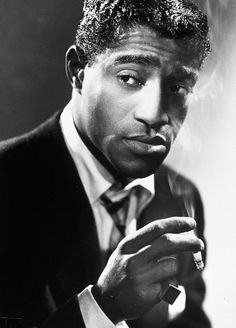
\includegraphics[width=0.5\linewidth]{images/sammy} 

}

\caption{The great Sammy Davis Jr. Do yourself a favor and spend an evening watching videos of him performing on YouTube. Image used entirely without permission.}\label{fig:sammy}
\end{figure}

Sammy Davis Jr. was one of the greatest American performers of all time.
If you don't know him already, Sammy was an American entertainer who
lived from 1925 to 1990. The range of his talents was just incredible.
He could sing, dance, act, and play multiple instruments with ease. So
how is R like Sammy Davis Jr? Like Sammy Davis Jr., R is incredibly good
at doing many different things. R does data analysis like Sammy dances,
and creates plot like Sammy sings. If Sammy and R did just one of these
things, they'd be great. The fact that they can do both is pretty
amazing.

When you evaluate plotting functions in R, R can build the plot in
different locations. The default location for plots is in a temporary
plotting window within your R programming environment. In RStudio, plots
will show up in the Plot window (typically on the bottom right hand
window pane). In Base R, plots will show up in a Quartz window.

You can think of these plotting locations as canvases. You only have one
canvas active at any given time, and any plotting command you run will
put more plotting elements on your active canvas. Certain high--level
plotting functions like \texttt{plot()} and \texttt{hist()} create brand
new canvases, while other low--level plotting functions like
\texttt{points()} and \texttt{segments()} place elements on top of
existing canvases.

Don't worry if that's confusing for now -- we'll go over all the details
soon.

Let's start by looking at a basic scatterplot in R using the
\texttt{plot()} function. When you execute the following code, you
should see a plot open in a new window:

\begin{Shaded}
\begin{Highlighting}[]
\CommentTok{# A basic scatterplot}
\KeywordTok{plot}\NormalTok{(}\DataTypeTok{x =} \DecValTok{1}\NormalTok{:}\DecValTok{10}\NormalTok{,}
     \DataTypeTok{y =} \DecValTok{1}\NormalTok{:}\DecValTok{10}\NormalTok{,}
     \DataTypeTok{xlab =} \StringTok{"X Axis label"}\NormalTok{,}
     \DataTypeTok{ylab =} \StringTok{"Y Axis label"}\NormalTok{,}
     \DataTypeTok{main =} \StringTok{"Main Title"}\NormalTok{)}
\end{Highlighting}
\end{Shaded}

\begin{center}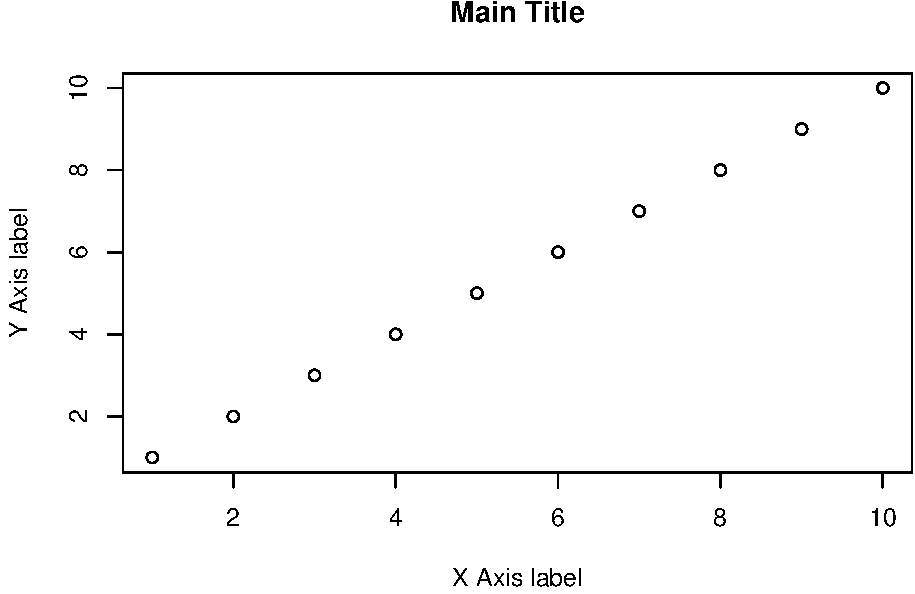
\includegraphics{YaRrr_files/figure-latex/basicplot-1} \end{center}

Let's take a look at the result. We see an x--axis, a y--axis, 10 data
points, an x--axis label, a y--axis label, and a main plot title. Some
of these items, like the labels and data points, were entered as
arguments to the function. For example, the main arguments x and y are
vectors indicating the x and y coordinates of the (in this case, 10)
data points. The arguments \texttt{xlab}, \texttt{ylab}, and
\texttt{main} set the labels to the plot. However, there were many
elements that I did not specify -- from the x and y axis limits, to the
color of the plotting points. As you'll discover later, you can change
all of these elements (and many, many more) by specifying additional
arguments to the \texttt{plot()} function. However, because I did not
specify them, R used \textbf{default} values -- values that R uses
unless you tell it to use something else.

For the rest of this chapter, we'll go over the main plotting functions,
along with the most common arguments you can use to customize the look
of your plot.

\section{Colors}\label{colors}

Most plotting functions have a color argument (usually \texttt{col})
that allows you to specify the color of whatever your plotting. There
are many ways to specify colors in R, let's start with the easiest ways.

\subsection{Colors by name}\label{colors-by-name}

The easiest way to specify a color is to enter its name as a string. For
example \texttt{col\ =\ "red"} is R's default version of the color red.
Of course, all the basic colors are there, but R also has tons of quirky
colors like \texttt{"snow"}, \texttt{"papayawhip"} and
\texttt{"lawngreen"}. Figure \ref{fig:randomcolors} shows 100 randomly
selected named colors.

\begin{figure}

{\centering 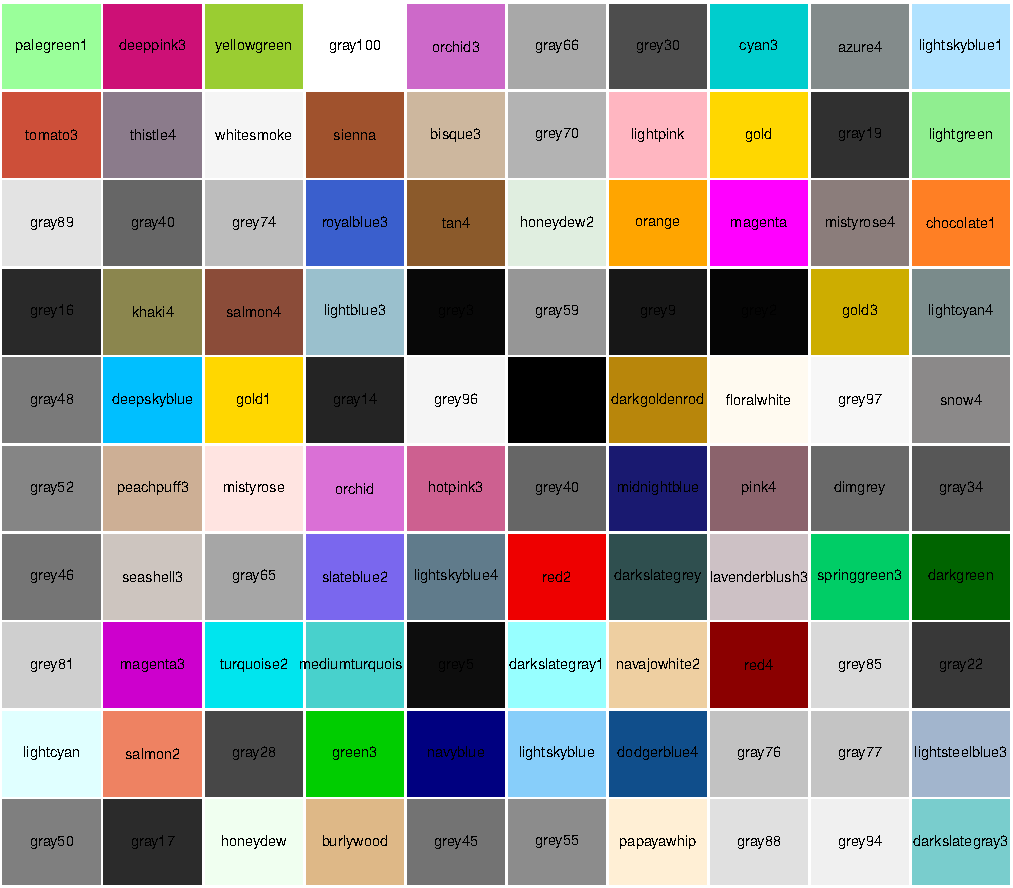
\includegraphics{YaRrr_files/figure-latex/randomcolors-1} 

}

\caption{100 random named colors (out of all 657) in R.}\label{fig:randomcolors}
\end{figure}

To see all 657 color names in R, run the code \texttt{colors()}. Or to
see an interactive demo of colors, run \texttt{demo("colors")}.

\subsection{gray()}\label{gray}

\begin{longtable}[]{@{}ll@{}}
\caption{\label{tab:gray} \texttt{gray()} function arguments}\tabularnewline
\toprule
\begin{minipage}[b]{0.18\columnwidth}\raggedright\strut
Argument\strut
\end{minipage} & \begin{minipage}[b]{0.67\columnwidth}\raggedright\strut
Description\strut
\end{minipage}\tabularnewline
\midrule
\endfirsthead
\toprule
\begin{minipage}[b]{0.18\columnwidth}\raggedright\strut
Argument\strut
\end{minipage} & \begin{minipage}[b]{0.67\columnwidth}\raggedright\strut
Description\strut
\end{minipage}\tabularnewline
\midrule
\endhead
\begin{minipage}[t]{0.18\columnwidth}\raggedright\strut
\texttt{level}\strut
\end{minipage} & \begin{minipage}[t]{0.67\columnwidth}\raggedright\strut
Lightness: \texttt{level\ =\ 1} = totally white, \texttt{level\ =\ 0} =
totally black\strut
\end{minipage}\tabularnewline
\begin{minipage}[t]{0.18\columnwidth}\raggedright\strut
\texttt{alpha}\strut
\end{minipage} & \begin{minipage}[t]{0.67\columnwidth}\raggedright\strut
Transparency: \texttt{alpha\ =\ 0} = totally transparent,
\texttt{alpha\ =\ 1} = not transparent at all.\strut
\end{minipage}\tabularnewline
\bottomrule
\end{longtable}

\begin{figure}

{\centering 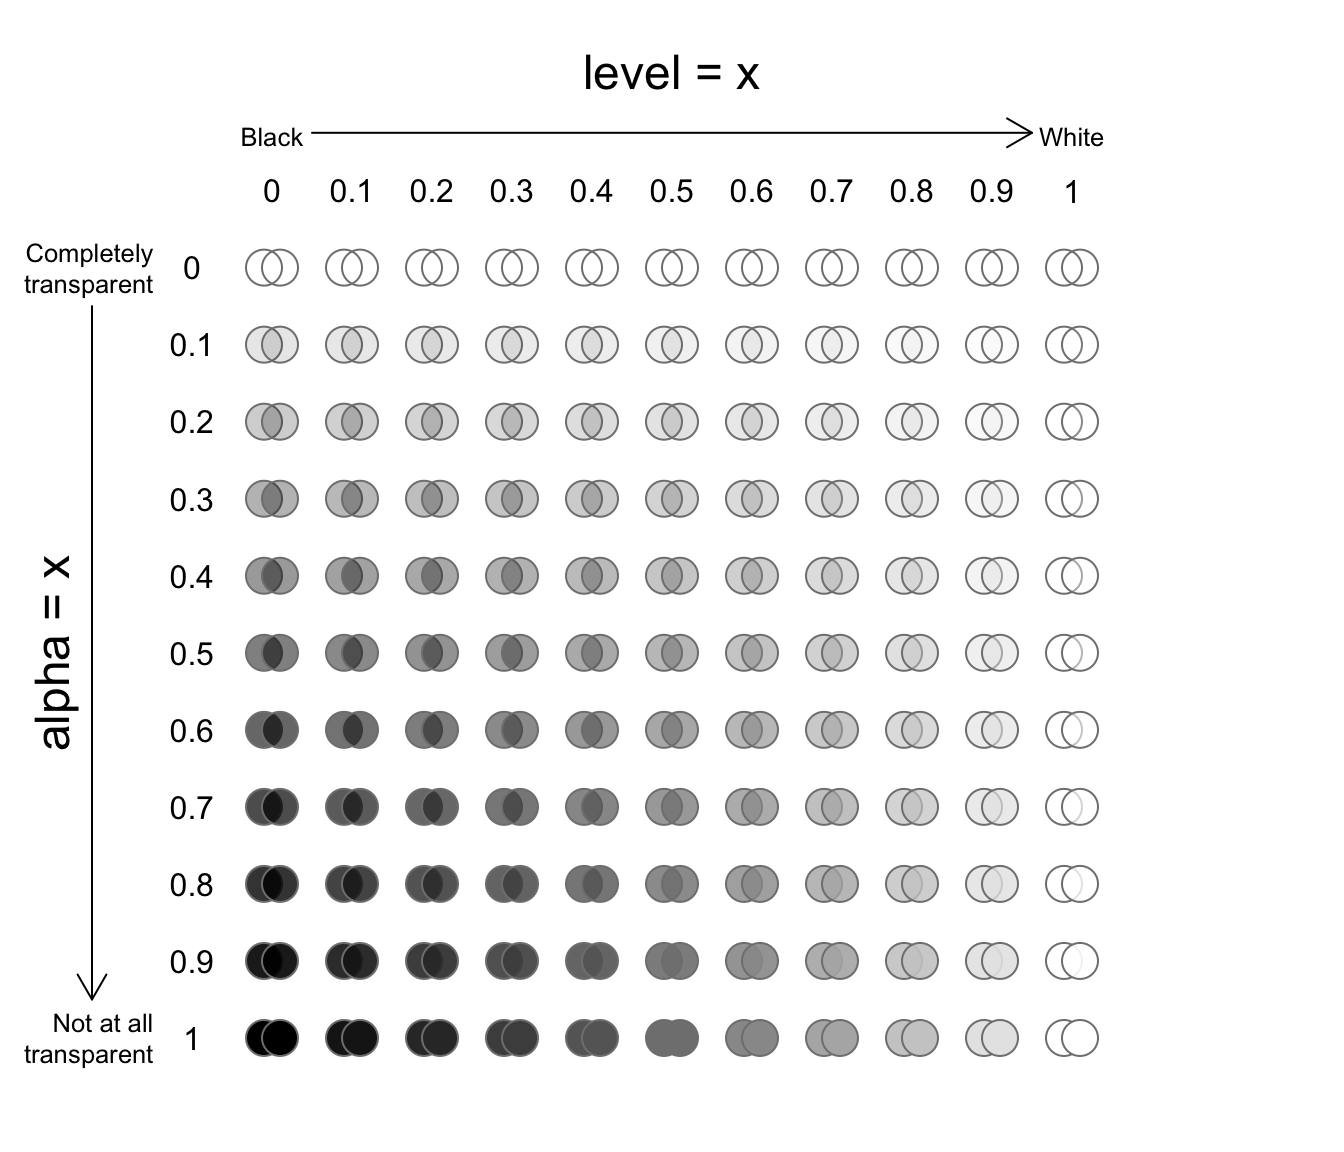
\includegraphics{YaRrr_files/figure-latex/graylevels-1} 

}

\caption{Examples of gray(level, alpha)}\label{fig:graylevels}
\end{figure}

If you're into erotic romance and BDSM, then you might be interested in
\href{https://en.wikipedia.org/wiki/Fifty_Shades_of_Grey}{Shades of
Gray}. If so, the function \texttt{gray(x)} is your answer. The
\texttt{gray()} function takes two arguments, \texttt{level} and
\texttt{alpha}, and returns a shade of gray. For example,
\texttt{gray(level\ =\ 1)} will return white. The second \texttt{alpha}
argument specifies how transparent to make the color on a scale from 0
(completely transparent), to 1 (not transparent at all). The default
value for alpha is 1 (not transparent at all). See Figure
\ref{fig:graylevels} for examples.

\subsection{\texorpdfstring{\texttt{yarrr::transparent()}}{yarrr::transparent()}}\label{yarrrtransparent}

I don't know about you, but I almost always find transparent colors to
be more appealing than solid colors. Not only do they help you see when
multiple points are overlapping, but they're just much nicer to look at.
Just look at the overlapping circles in the plot below.

\begin{center}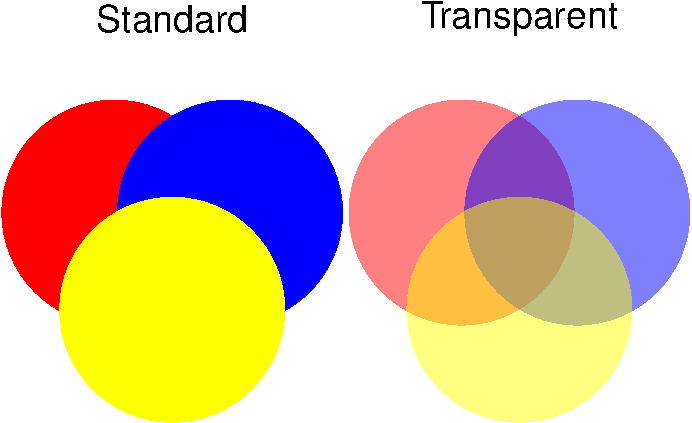
\includegraphics{YaRrr_files/figure-latex/unnamed-chunk-3-1} \end{center}

Unfortunately, as far as I know, base-R does not make it easy to make
transparent colors. Thankfully, there is a function in the
\texttt{yarrr} package called \texttt{transparent} that makes it very
easy to make any color transparent. To use it, just enter the original
color as the main argument \texttt{orig.col}, then enter how transparent
you want to make it (from 0 to 1) as the second argument
\texttt{trans.val}.

Here is a basic scatterplot with standard (non-transparent) colors:

\begin{Shaded}
\begin{Highlighting}[]
\CommentTok{# Plot with Standard Colors}
\KeywordTok{plot}\NormalTok{(}\DataTypeTok{x =} \NormalTok{pirates$height, }
     \DataTypeTok{y =} \NormalTok{pirates$weight, }
     \DataTypeTok{col =} \StringTok{"blue"}\NormalTok{, }
     \DataTypeTok{pch =} \DecValTok{16}\NormalTok{, }
     \DataTypeTok{main =} \StringTok{"col ='blue'"}\NormalTok{)}
\end{Highlighting}
\end{Shaded}

\begin{center}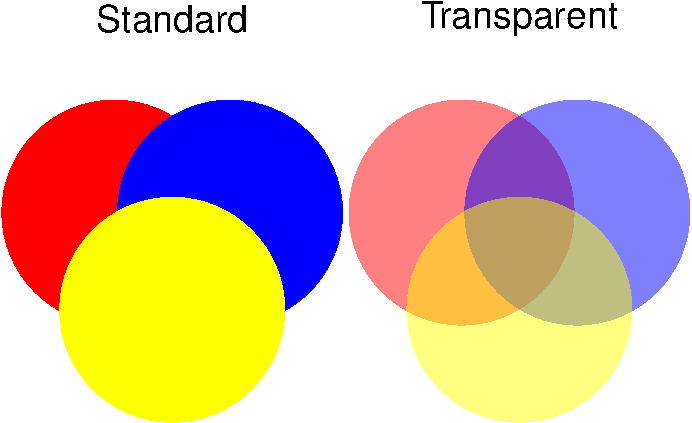
\includegraphics{YaRrr_files/figure-latex/unnamed-chunk-4-1} \end{center}

Now here's the same plot using the \texttt{transparent()} function in
the \texttt{yarrr} package:

\begin{Shaded}
\begin{Highlighting}[]
\CommentTok{# Plot with transparent colors using the transparent() function in the yarrr package}
\KeywordTok{plot}\NormalTok{(}\DataTypeTok{x =} \NormalTok{pirates$height, }
     \DataTypeTok{y =} \NormalTok{pirates$weight, }
     \DataTypeTok{col =} \NormalTok{yarrr::}\KeywordTok{transparent}\NormalTok{(}\StringTok{"blue"}\NormalTok{, }\DataTypeTok{trans.val =} \NormalTok{.}\DecValTok{9}\NormalTok{), }
     \DataTypeTok{pch =} \DecValTok{16}\NormalTok{, }
     \DataTypeTok{main =} \StringTok{"col = yarrr::transparent('blue', .9)"}\NormalTok{)}
\end{Highlighting}
\end{Shaded}

\begin{center}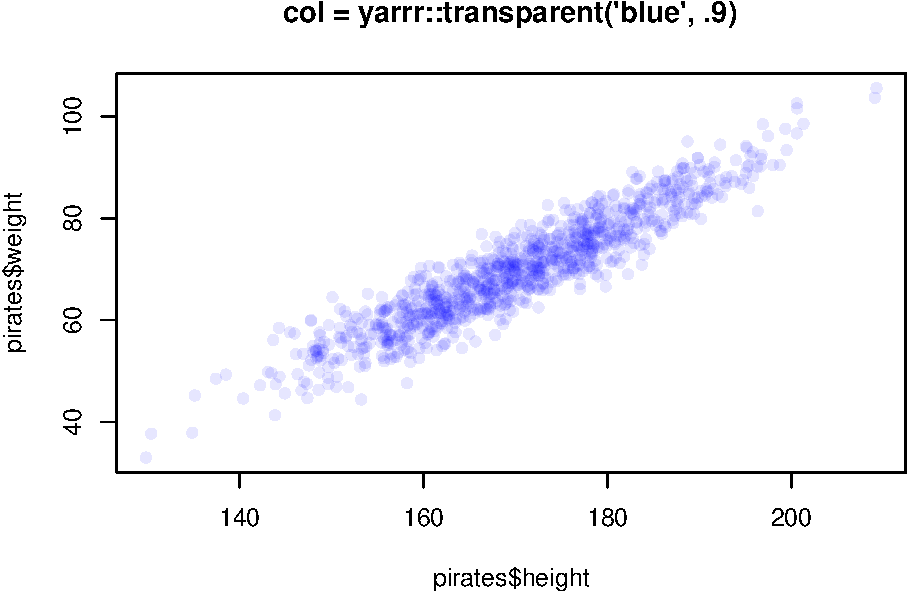
\includegraphics{YaRrr_files/figure-latex/unnamed-chunk-5-1} \end{center}

Later on in the book, we'll cover more advanced ways to come up with
colors using color palettes (using the RColorBrewer package or the
\texttt{piratepal()} function in the yarrr package) and functions that
generate shades of colors based on numeric data (like the
\texttt{colorRamp2()} function in the \texttt{circlize} package).

\section{Plotting arguments}\label{plotting-arguments}

Most plotting functions have \emph{tons} of optional arguments (also
called parameters) that you can use to customize virtually everything in
a plot. To see all of them, look at the help menu for \texttt{par} by
executing \texttt{?par}. However, the good news is that you don't need
to specify all possible parameters you create a plot. Instead, there are
only a few critical arguments that you must specify - usually one or two
vectors of data. For any optional arguments that you do not specify, R
will use either a default value, or choose a value that makes sense
based on the data you specify.

In the following examples, I will to cover the main plotting parameters
for each plotting type. However, the best way to learn what you can, and
can't, do with plots, is to try to create them yourself!

I think the best way to learn how to create plots is to see some
examples. Let's start with the main high-level plotting functions.

\section{\texorpdfstring{Scatterplot:
\texttt{plot()}}{Scatterplot: plot()}}\label{scatterplot-plot}

The most common high-level plotting function is \texttt{plot(x,\ y)}.
The \texttt{plot()} function makes a scatterplot from two vectors x and
y, where the x vector indicates the x (horizontal) values of the points,
and the y vector indicates the y (vertical) values.

\begin{longtable}[]{@{}ll@{}}
\caption{\label{tab:plot} \texttt{plot()} function arguments}\tabularnewline
\toprule
\begin{minipage}[b]{0.18\columnwidth}\raggedright\strut
Argument\strut
\end{minipage} & \begin{minipage}[b]{0.67\columnwidth}\raggedright\strut
Description\strut
\end{minipage}\tabularnewline
\midrule
\endfirsthead
\toprule
\begin{minipage}[b]{0.18\columnwidth}\raggedright\strut
Argument\strut
\end{minipage} & \begin{minipage}[b]{0.67\columnwidth}\raggedright\strut
Description\strut
\end{minipage}\tabularnewline
\midrule
\endhead
\begin{minipage}[t]{0.18\columnwidth}\raggedright\strut
\texttt{x,\ y}\strut
\end{minipage} & \begin{minipage}[t]{0.67\columnwidth}\raggedright\strut
Vectors of equal length specifying the x and y values of the
points\strut
\end{minipage}\tabularnewline
\begin{minipage}[t]{0.18\columnwidth}\raggedright\strut
\texttt{type}\strut
\end{minipage} & \begin{minipage}[t]{0.67\columnwidth}\raggedright\strut
Type of plot. \texttt{"l"} means lines, \texttt{"p"} means points,
\texttt{"b"} means lines and points, \texttt{"n"} means no
plotting\strut
\end{minipage}\tabularnewline
\begin{minipage}[t]{0.18\columnwidth}\raggedright\strut
\texttt{main}, \texttt{xlab}, \texttt{ylab}\strut
\end{minipage} & \begin{minipage}[t]{0.67\columnwidth}\raggedright\strut
Strings giving labels for the plot title, and x and y axes\strut
\end{minipage}\tabularnewline
\begin{minipage}[t]{0.18\columnwidth}\raggedright\strut
\texttt{xlim}, \texttt{ylim}\strut
\end{minipage} & \begin{minipage}[t]{0.67\columnwidth}\raggedright\strut
Limits to the axes. For example, \texttt{xlim\ =\ c(0,\ 100)} will set
the minimum and maximum of the x-axis to 0 and 100.\strut
\end{minipage}\tabularnewline
\begin{minipage}[t]{0.18\columnwidth}\raggedright\strut
\texttt{pch}\strut
\end{minipage} & \begin{minipage}[t]{0.67\columnwidth}\raggedright\strut
An integer indicating the type of plotting symbols (see \texttt{?points}
and section below), or a string specifying symbols as text. For example,
\texttt{pch\ =\ 21} will create a two-color circle, while
\texttt{pch\ =\ "P"} will plot the character \texttt{"P"}. To see all
the different symbol types, run \texttt{?points}.\strut
\end{minipage}\tabularnewline
\begin{minipage}[t]{0.18\columnwidth}\raggedright\strut
\texttt{col}\strut
\end{minipage} & \begin{minipage}[t]{0.67\columnwidth}\raggedright\strut
Main color of the plotting symbols. For example \texttt{col\ =\ "red"}
will create red symbols.\strut
\end{minipage}\tabularnewline
\begin{minipage}[t]{0.18\columnwidth}\raggedright\strut
\texttt{cex}\strut
\end{minipage} & \begin{minipage}[t]{0.67\columnwidth}\raggedright\strut
A numeric vector specifying the size of the symbols (from 0 to Inf). The
default size is 1. \texttt{cex\ =\ 4} will make the points very large,
while \texttt{cex\ =\ .5} will make them very small.\strut
\end{minipage}\tabularnewline
\bottomrule
\end{longtable}

\begin{Shaded}
\begin{Highlighting}[]
\KeywordTok{plot}\NormalTok{(}\DataTypeTok{x =} \DecValTok{1}\NormalTok{:}\DecValTok{10}\NormalTok{,                         }\CommentTok{# x-coordinates}
     \DataTypeTok{y =} \DecValTok{1}\NormalTok{:}\DecValTok{10}\NormalTok{,                         }\CommentTok{# y-coordinates}
     \DataTypeTok{type =} \StringTok{"p"}\NormalTok{,                       }\CommentTok{# Just draw points (no lines)}
     \DataTypeTok{main =} \StringTok{"My First Plot"}\NormalTok{,}
     \DataTypeTok{xlab =} \StringTok{"This is the x-axis label"}\NormalTok{,}
     \DataTypeTok{ylab =} \StringTok{"This is the y-axis label"}\NormalTok{,}
     \DataTypeTok{xlim =} \KeywordTok{c}\NormalTok{(}\DecValTok{0}\NormalTok{, }\DecValTok{11}\NormalTok{),                  }\CommentTok{# Min and max values for x-axis}
     \DataTypeTok{ylim =} \KeywordTok{c}\NormalTok{(}\DecValTok{0}\NormalTok{, }\DecValTok{11}\NormalTok{),                  }\CommentTok{# Min and max values for y-axis}
     \DataTypeTok{col =} \StringTok{"blue"}\NormalTok{,                     }\CommentTok{# Color of the points}
     \DataTypeTok{pch =} \DecValTok{16}\NormalTok{,                         }\CommentTok{# Type of symbol (16 means Filled circle)}
     \DataTypeTok{cex =} \DecValTok{1}\NormalTok{)                           }\CommentTok{# Size of the symbols}
\end{Highlighting}
\end{Shaded}

\begin{center}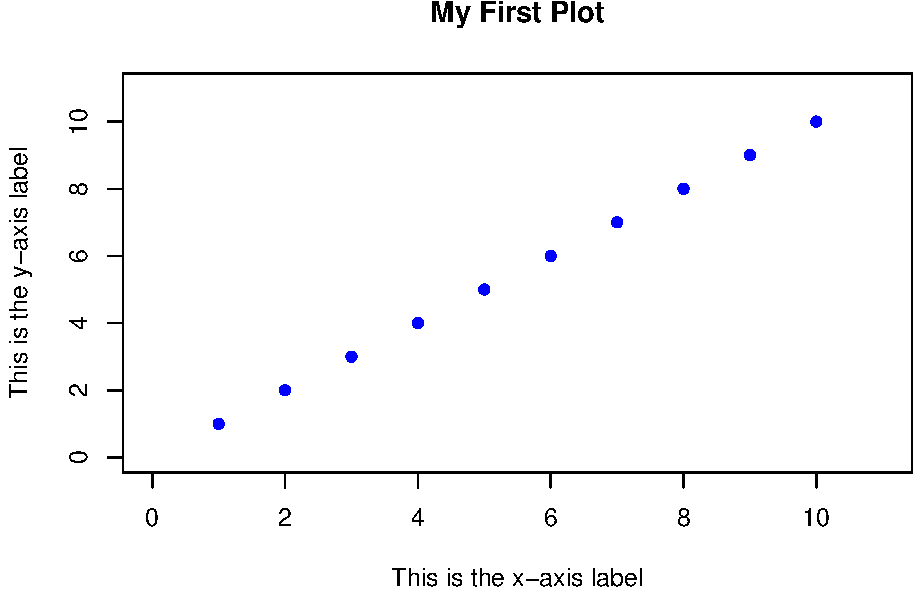
\includegraphics{YaRrr_files/figure-latex/unnamed-chunk-6-1} \end{center}

Aside from the x and y arguments, all of the arguments are optional. If
you don't specify a specific argument, then R will use a default value,
or try to come up with a value that makes sense. For example, if you
don't specify the \texttt{xlim} and \texttt{ylim} arguments, R will set
the limits so that all the points fit inside the plot.

\subsection{\texorpdfstring{Symbol types:
\texttt{pch}}{Symbol types: pch}}\label{symbol-types-pch}

When you create a plot with \texttt{plot()} (or points with
\texttt{points()}), you can specify the type of symbol with the
\texttt{pch} argument. You can specify the symbol type in one of two
ways: with an integer, or with a string. If you use a string (like
\texttt{"p"}), R will use that text as the plotting symbol. If you use
an integer value, you'll get the symbol that correspond to that number.
See Figure for all the symbol types you can specify with an integer.

Symbols differ in their shape and how they are colored. Symbols 1
through 14 only have borders and are always empty, while symbols 15
through 20 don't have a border and are always filled. Symbols 21 through
25 have both a border and a filling. To specify the border color or
background for symbols 1 through 20, use the \texttt{col} argument. For
symbols 21 through 25, you set the color of the border with
\texttt{col}, and the color of the background using \texttt{bg}

\begin{figure}

{\centering 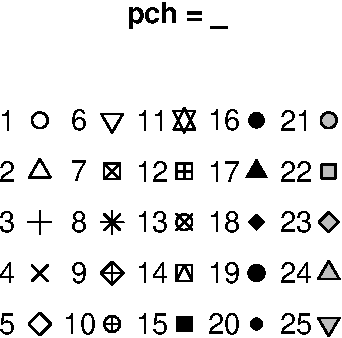
\includegraphics{YaRrr_files/figure-latex/unnamed-chunk-7-1} 

}

\caption{The symbol types associated with the pch plotting parameter.}\label{fig:unnamed-chunk-7}
\end{figure}

Let's look at some different symbol types in action when applied to the
same data:

\begin{center}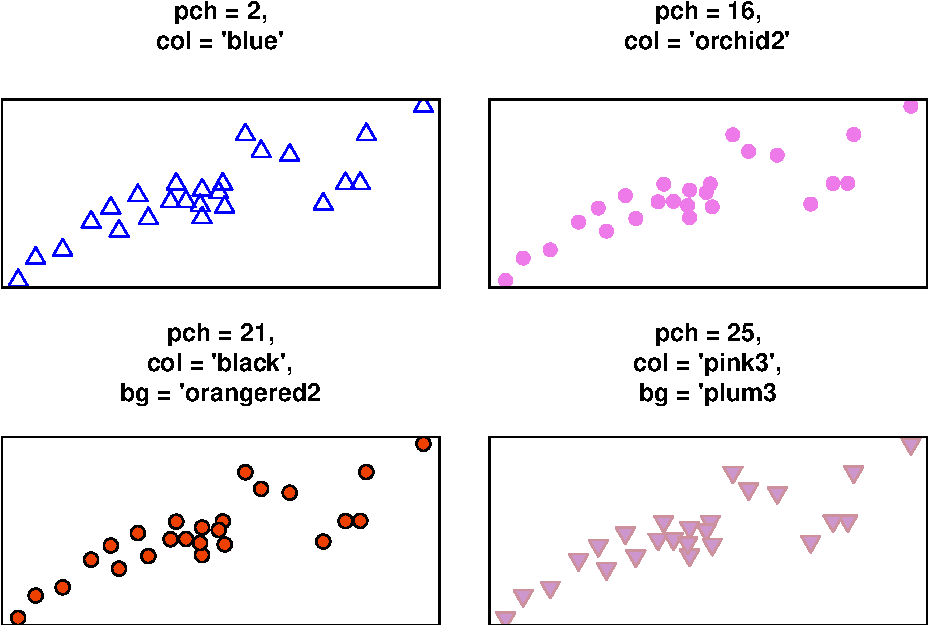
\includegraphics{YaRrr_files/figure-latex/unnamed-chunk-8-1} \end{center}

\section{\texorpdfstring{Histogram:
\texttt{hist()}}{Histogram: hist()}}\label{histogram-hist}

\begin{longtable}[]{@{}ll@{}}
\caption{\label{tab:hist} \texttt{hist()} function arguments}\tabularnewline
\toprule
\begin{minipage}[b]{0.18\columnwidth}\raggedright\strut
Argument\strut
\end{minipage} & \begin{minipage}[b]{0.67\columnwidth}\raggedright\strut
Description\strut
\end{minipage}\tabularnewline
\midrule
\endfirsthead
\toprule
\begin{minipage}[b]{0.18\columnwidth}\raggedright\strut
Argument\strut
\end{minipage} & \begin{minipage}[b]{0.67\columnwidth}\raggedright\strut
Description\strut
\end{minipage}\tabularnewline
\midrule
\endhead
\begin{minipage}[t]{0.18\columnwidth}\raggedright\strut
\texttt{x}\strut
\end{minipage} & \begin{minipage}[t]{0.67\columnwidth}\raggedright\strut
Vector of values\strut
\end{minipage}\tabularnewline
\begin{minipage}[t]{0.18\columnwidth}\raggedright\strut
\texttt{breaks}\strut
\end{minipage} & \begin{minipage}[t]{0.67\columnwidth}\raggedright\strut
How should the bin sizes be calculated? Can be specified in many ways
(see \texttt{?hist} for details)\strut
\end{minipage}\tabularnewline
\begin{minipage}[t]{0.18\columnwidth}\raggedright\strut
\texttt{freq}\strut
\end{minipage} & \begin{minipage}[t]{0.67\columnwidth}\raggedright\strut
Should frequencies or probabilities be plotted? \texttt{freq\ =\ TRUE}
shows frequencies, \texttt{freq\ =\ FALSE} shows probabilities.\strut
\end{minipage}\tabularnewline
\begin{minipage}[t]{0.18\columnwidth}\raggedright\strut
\texttt{col}, \texttt{border}\strut
\end{minipage} & \begin{minipage}[t]{0.67\columnwidth}\raggedright\strut
Colors of the bin filling (\texttt{col}) and border
(\texttt{border})\strut
\end{minipage}\tabularnewline
\bottomrule
\end{longtable}

Histograms are the most common way to plot a vector of numeric data. To
create a histogram we'll use the \texttt{hist()} function. The main
argument to \texttt{hist()} is a \texttt{x}, a vector of numeric data.
If you want to specify how the histogram bins are created, you can use
the \texttt{breaks} argument. To change the color of the border or
background of the bins, use \texttt{col} and \texttt{border}:

Let's create a histogram of the weights in the ChickWeight dataset:

\begin{Shaded}
\begin{Highlighting}[]
\KeywordTok{hist}\NormalTok{(}\DataTypeTok{x =} \NormalTok{ChickWeight$weight,}
     \DataTypeTok{main =} \StringTok{"Chicken Weights"}\NormalTok{,}
     \DataTypeTok{xlab =} \StringTok{"Weight"}\NormalTok{,}
     \DataTypeTok{xlim =} \KeywordTok{c}\NormalTok{(}\DecValTok{0}\NormalTok{, }\DecValTok{500}\NormalTok{))}
\end{Highlighting}
\end{Shaded}

\begin{center}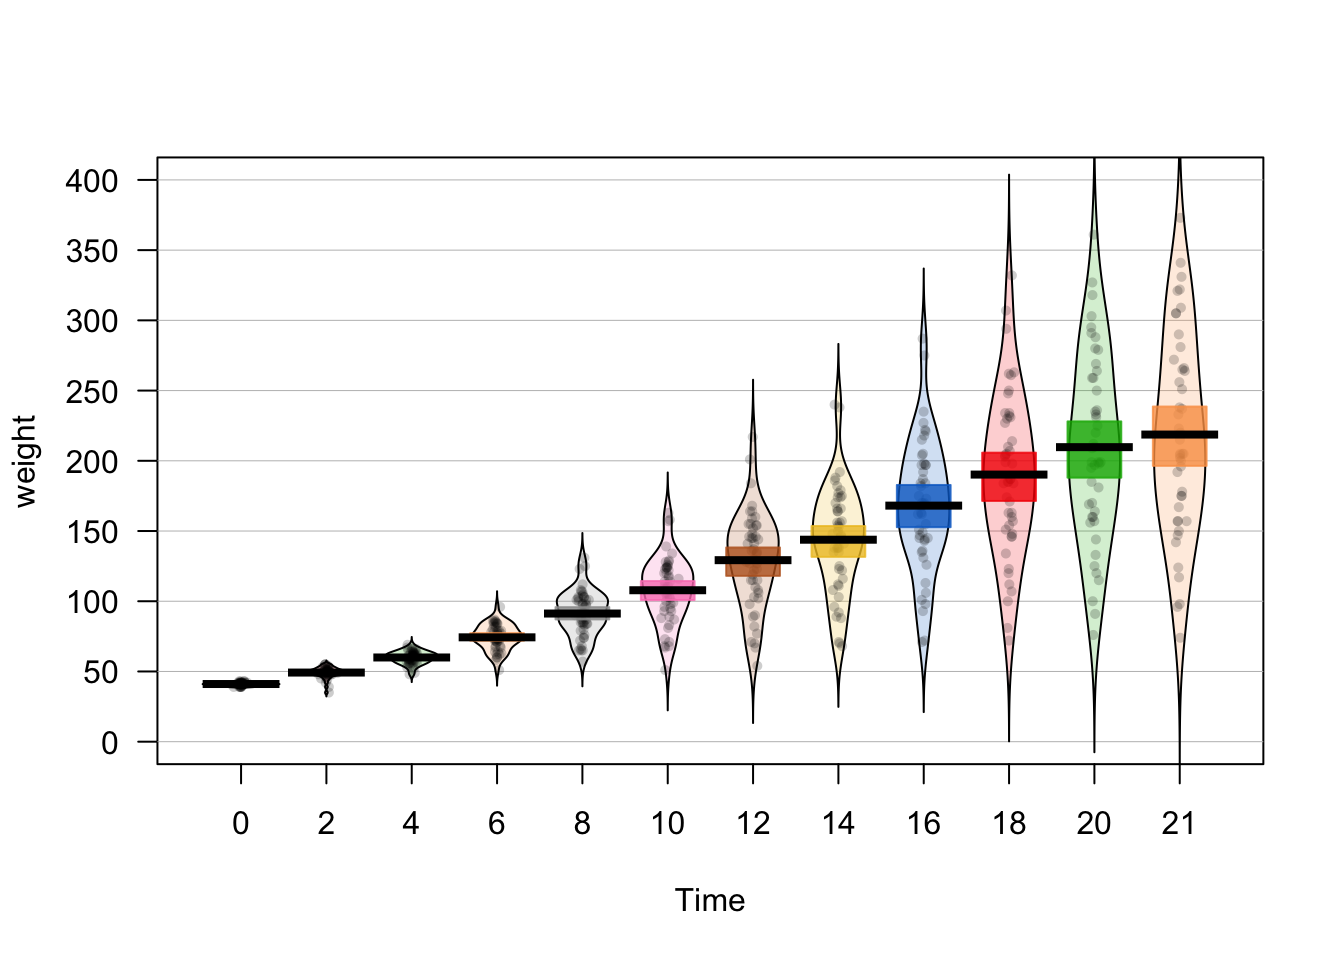
\includegraphics{YaRrr_files/figure-latex/unnamed-chunk-9-1} \end{center}

We can get more fancy by adding additional arguments like
\texttt{breaks\ =\ 20} to force there to be 20 bins, and
\texttt{col\ =\ "papayawhip"} and \texttt{bg\ =\ "hotpink"} to make it a
bit more colorful:

\begin{Shaded}
\begin{Highlighting}[]
\KeywordTok{hist}\NormalTok{(}\DataTypeTok{x =} \NormalTok{ChickWeight$weight,}
     \DataTypeTok{main =} \StringTok{"Fancy Chicken Weight Histogram"}\NormalTok{,}
     \DataTypeTok{xlab =} \StringTok{"Weight"}\NormalTok{,}
     \DataTypeTok{ylab =} \StringTok{"Frequency"}\NormalTok{,}
     \DataTypeTok{breaks =} \DecValTok{20}\NormalTok{, }\CommentTok{# 20 Bins}
     \DataTypeTok{xlim =} \KeywordTok{c}\NormalTok{(}\DecValTok{0}\NormalTok{, }\DecValTok{500}\NormalTok{),}
     \DataTypeTok{col =} \StringTok{"papayawhip"}\NormalTok{, }\CommentTok{# Filling Color}
     \DataTypeTok{border =} \StringTok{"hotpink"}\NormalTok{) }\CommentTok{# Border Color}
\end{Highlighting}
\end{Shaded}

\begin{center}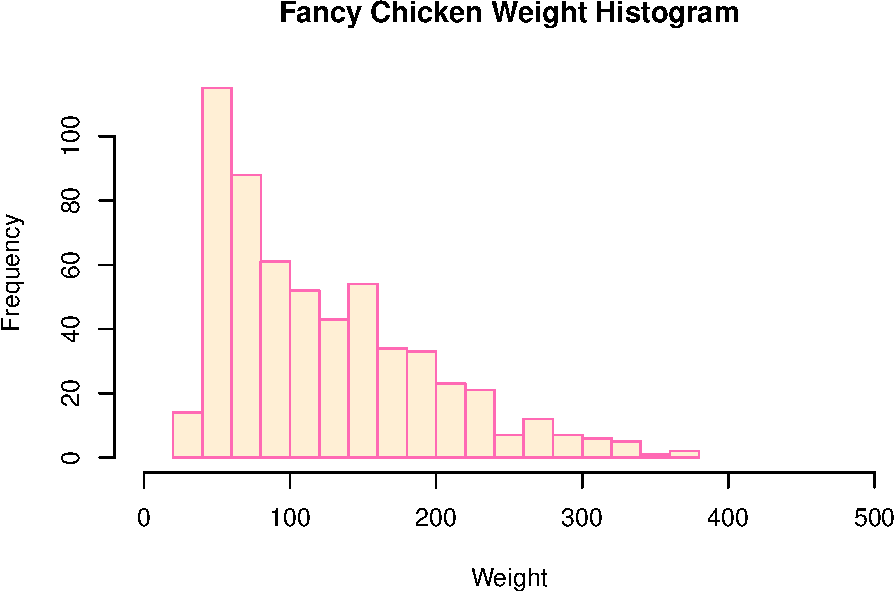
\includegraphics{YaRrr_files/figure-latex/unnamed-chunk-10-1} \end{center}

If you want to plot two histograms on the same plot, for example, to
show the distributions of two different groups, you can use the
\texttt{add = TRUE} argument to the second plot.

\begin{Shaded}
\begin{Highlighting}[]
\KeywordTok{hist}\NormalTok{(}\DataTypeTok{x =} \NormalTok{ChickWeight$weight[ChickWeight$Diet ==}\StringTok{ }\DecValTok{1}\NormalTok{],}
     \DataTypeTok{main =} \StringTok{"Two Histograms in one"}\NormalTok{,}
     \DataTypeTok{xlab =} \StringTok{"Weight"}\NormalTok{,}
     \DataTypeTok{ylab =} \StringTok{"Frequency"}\NormalTok{,}
     \DataTypeTok{breaks =} \DecValTok{20}\NormalTok{,}
     \DataTypeTok{xlim =} \KeywordTok{c}\NormalTok{(}\DecValTok{0}\NormalTok{, }\DecValTok{500}\NormalTok{),}
     \DataTypeTok{col =} \KeywordTok{gray}\NormalTok{(}\DecValTok{0}\NormalTok{, .}\DecValTok{5}\NormalTok{))}

\KeywordTok{hist}\NormalTok{(}\DataTypeTok{x =} \NormalTok{ChickWeight$weight[ChickWeight$Diet ==}\StringTok{ }\DecValTok{2}\NormalTok{],}
     \DataTypeTok{breaks =} \DecValTok{30}\NormalTok{,}
     \DataTypeTok{add =} \OtherTok{TRUE}\NormalTok{, }\CommentTok{# Add plot to previous one!}
     \DataTypeTok{col =} \KeywordTok{gray}\NormalTok{(}\DecValTok{1}\NormalTok{, .}\DecValTok{8}\NormalTok{))}
\end{Highlighting}
\end{Shaded}

\begin{center}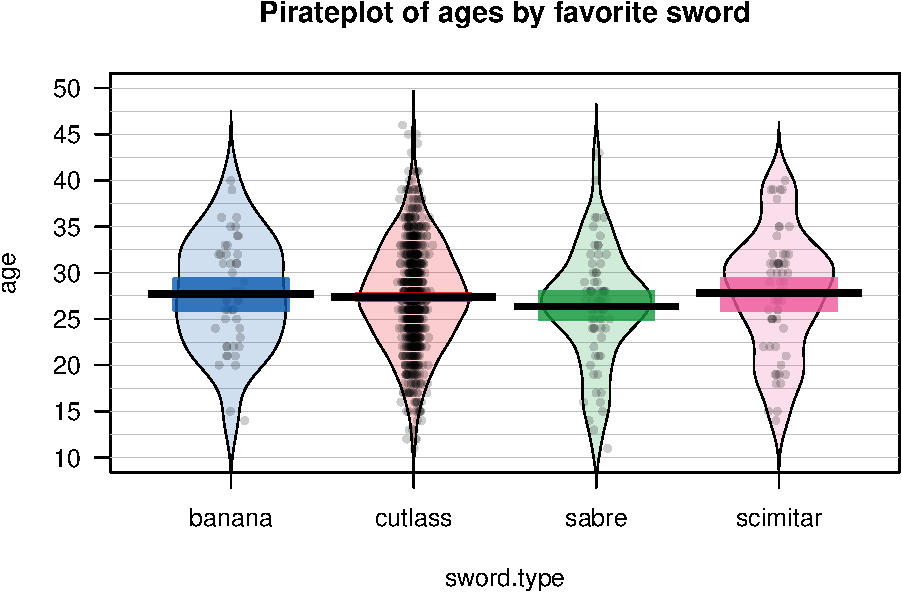
\includegraphics{YaRrr_files/figure-latex/unnamed-chunk-11-1} \end{center}

\section{\texorpdfstring{Barplot:
\texttt{barplot()}}{Barplot: barplot()}}\label{barplot-barplot}

A barplot typically shows summary statistics for different groups. The
primary argument to a barplot is \texttt{height}: a vector of numeric
values which will generate the height of each bar. To add names below
the bars, use the \texttt{names.arg} argument. For additional arguments
specific to \texttt{barplot()}, look at the help menu with
\texttt{?barplot}:

\begin{Shaded}
\begin{Highlighting}[]
\KeywordTok{barplot}\NormalTok{(}\DataTypeTok{height =} \DecValTok{1}\NormalTok{:}\DecValTok{5}\NormalTok{,  }\CommentTok{# A vector of heights}
        \DataTypeTok{names.arg =} \KeywordTok{c}\NormalTok{(}\StringTok{"G1"}\NormalTok{, }\StringTok{"G2"}\NormalTok{, }\StringTok{"G3"}\NormalTok{, }\StringTok{"G4"}\NormalTok{, }\StringTok{"G5"}\NormalTok{), }\CommentTok{# A vector of names}
        \DataTypeTok{main =} \StringTok{"Example Barplot"}\NormalTok{, }
        \DataTypeTok{xlab =} \StringTok{"Group"}\NormalTok{, }
        \DataTypeTok{ylab =} \StringTok{"Height"}\NormalTok{)}
\end{Highlighting}
\end{Shaded}

\begin{center}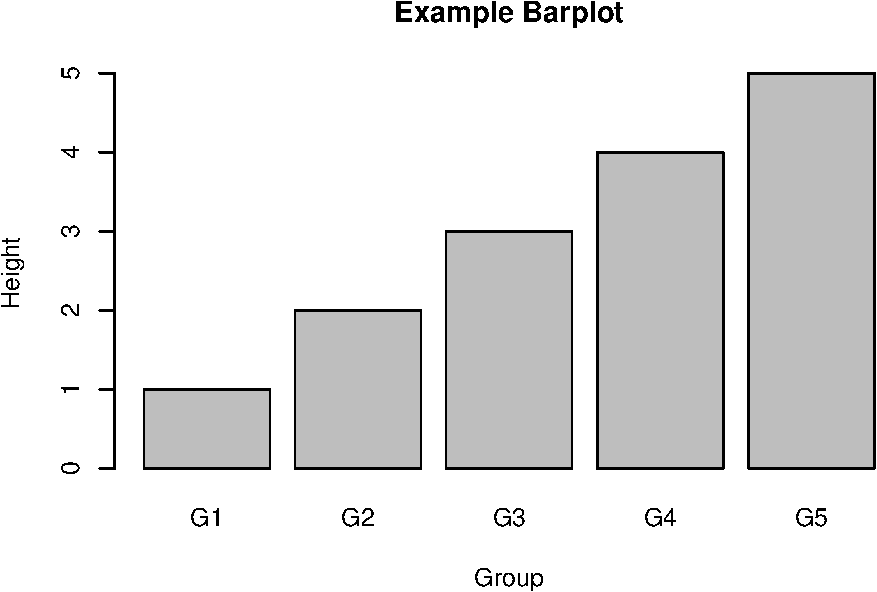
\includegraphics{YaRrr_files/figure-latex/unnamed-chunk-12-1} \end{center}

Of course, you should plot more interesting data than just a vector of
integers with a barplot. In the plot below, I create a barplot with the
average weight of chickens for each week:

\begin{Shaded}
\begin{Highlighting}[]
\CommentTok{# Calculate mean weights for each time period}
\NormalTok{diet.weights <-}\StringTok{ }\KeywordTok{aggregate}\NormalTok{(weight ~}\StringTok{ }\NormalTok{Time, }
                      \DataTypeTok{data =} \NormalTok{ChickWeight,}
                      \DataTypeTok{FUN =} \NormalTok{mean)}

\CommentTok{# Create barplot}
\KeywordTok{barplot}\NormalTok{(}\DataTypeTok{height =} \NormalTok{diet.weights$weight,}
        \DataTypeTok{names.arg =} \NormalTok{diet.weights$Time,}
        \DataTypeTok{xlab =} \StringTok{"Week"}\NormalTok{,}
        \DataTypeTok{ylab =} \StringTok{"Average Weight"}\NormalTok{,}
        \DataTypeTok{main =} \StringTok{"Average Chicken Weights by Time"}\NormalTok{,}
        \DataTypeTok{col =} \StringTok{"mistyrose"}\NormalTok{)}
\end{Highlighting}
\end{Shaded}

\begin{center}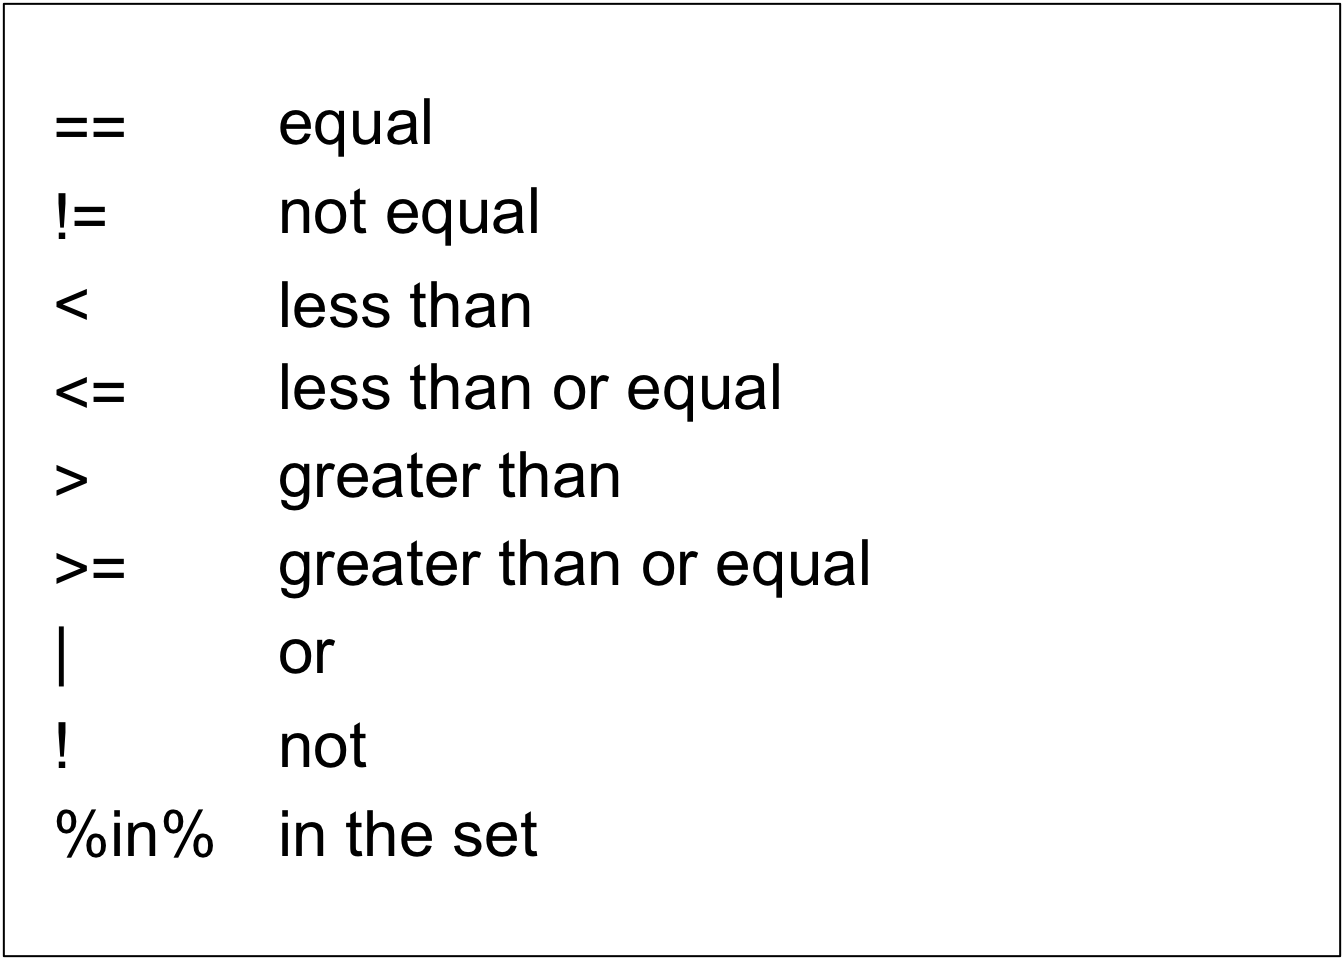
\includegraphics{YaRrr_files/figure-latex/unnamed-chunk-13-1} \end{center}

\subsection{Clustered barplot}\label{clustered-barplot}

If you want to create a clustered barplot, with different bars for
different groups of data, you can enter a matrix as the argument to
\texttt{height}. R will then plot each column of the matrix as a
separate set of bars. For example, let's say I conducted an experiment
where I compared how fast pirates can swim under four conditions:
Wearing clothes versus being naked, and while being chased by a shark
versus not being chased by a shark. Let's say I conducted this
experiment and calculated the following average swimming speed:

\begin{tabular}{l|r|r}
\hline
  & Naked & Clothed\\
\hline
No Shark & 2.1 & 1.5\\
\hline
Shark & 3.0 & 3.0\\
\hline
\end{tabular}

I can represent these data in a matrix as follows. In order for the
final barplot to include the condition names, I'll add row and column
names to the matrix with \texttt{colnames()} and \texttt{rownames()}

\begin{Shaded}
\begin{Highlighting}[]
\NormalTok{swim.data <-}\StringTok{ }\KeywordTok{cbind}\NormalTok{(}\KeywordTok{c}\NormalTok{(}\FloatTok{2.1}\NormalTok{, }\DecValTok{3}\NormalTok{), }\CommentTok{# Naked Times}
                   \KeywordTok{c}\NormalTok{(}\FloatTok{1.5}\NormalTok{, }\DecValTok{3}\NormalTok{)) }\CommentTok{# Clothed Times}

\KeywordTok{colnames}\NormalTok{(swim.data) <-}\StringTok{ }\KeywordTok{c}\NormalTok{(}\StringTok{"Naked"}\NormalTok{, }\StringTok{"Clothed"}\NormalTok{)}
\KeywordTok{rownames}\NormalTok{(swim.data) <-}\StringTok{ }\KeywordTok{c}\NormalTok{(}\StringTok{"No Shark"}\NormalTok{, }\StringTok{"Shark"}\NormalTok{)}

\CommentTok{# Print result}
\NormalTok{swim.data}
\NormalTok{##          Naked Clothed}
\NormalTok{## No Shark   2.1     1.5}
\NormalTok{## Shark      3.0     3.0}
\end{Highlighting}
\end{Shaded}

Now, when I enter this matrix as the \texttt{height\ =\ swim.data}
argument to \texttt{barplot()}, I'll get multiple bars.

\begin{Shaded}
\begin{Highlighting}[]
\KeywordTok{barplot}\NormalTok{(}\DataTypeTok{height =} \NormalTok{swim.data,}
        \DataTypeTok{beside =} \OtherTok{TRUE}\NormalTok{,                        }\CommentTok{# Put the bars next to each other}
        \DataTypeTok{legend.text =} \OtherTok{TRUE}\NormalTok{,                   }\CommentTok{# Add a legend}
        \DataTypeTok{col =} \KeywordTok{c}\NormalTok{(}\KeywordTok{transparent}\NormalTok{(}\StringTok{"green"}\NormalTok{, .}\DecValTok{2}\NormalTok{), }
                \KeywordTok{transparent}\NormalTok{(}\StringTok{"red"}\NormalTok{, .}\DecValTok{2}\NormalTok{)),}
        \DataTypeTok{main =} \StringTok{"Swimming Speed Experiment"}\NormalTok{,}
        \DataTypeTok{ylab =} \StringTok{"Speed (in meters / second)"}\NormalTok{,}
        \DataTypeTok{xlab =} \StringTok{"Clothing Condition"}\NormalTok{,}
        \DataTypeTok{ylim =} \KeywordTok{c}\NormalTok{(}\DecValTok{0}\NormalTok{, }\DecValTok{4}\NormalTok{))}
\end{Highlighting}
\end{Shaded}

\begin{center}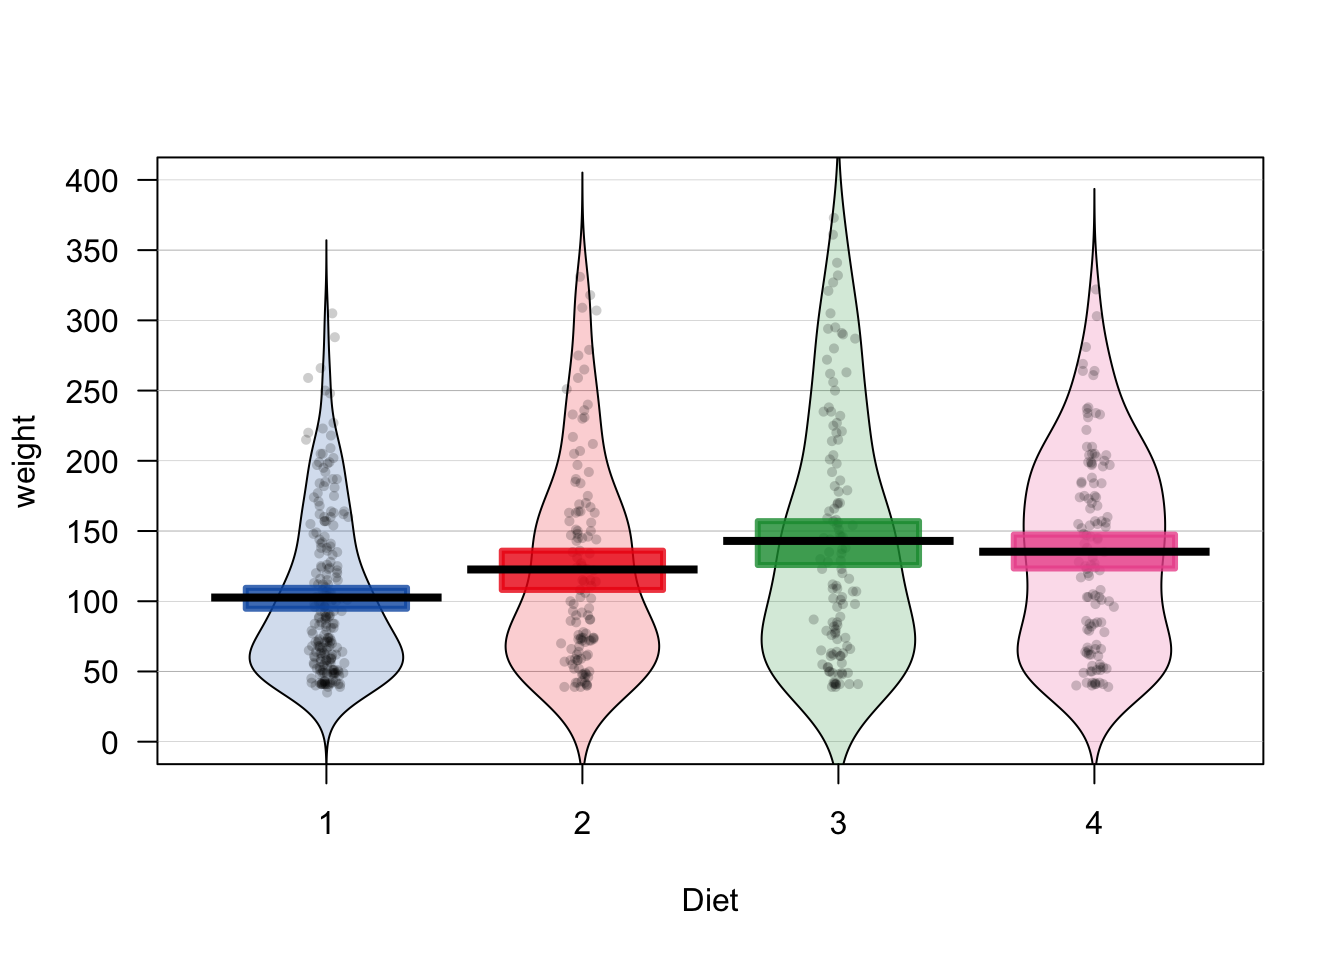
\includegraphics{YaRrr_files/figure-latex/unnamed-chunk-16-1} \end{center}

\section{\texorpdfstring{\texttt{pirateplot()}}{pirateplot()}}\label{pirateplot}

\begin{longtable}[]{@{}ll@{}}
\caption{\label{tab:pirateplot} \texttt{pirateplot()} function
arguments}\tabularnewline
\toprule
\begin{minipage}[b]{0.18\columnwidth}\raggedright\strut
Argument\strut
\end{minipage} & \begin{minipage}[b]{0.67\columnwidth}\raggedright\strut
Description\strut
\end{minipage}\tabularnewline
\midrule
\endfirsthead
\toprule
\begin{minipage}[b]{0.18\columnwidth}\raggedright\strut
Argument\strut
\end{minipage} & \begin{minipage}[b]{0.67\columnwidth}\raggedright\strut
Description\strut
\end{minipage}\tabularnewline
\midrule
\endhead
\begin{minipage}[t]{0.18\columnwidth}\raggedright\strut
\texttt{formula}\strut
\end{minipage} & \begin{minipage}[t]{0.67\columnwidth}\raggedright\strut
A formula specifying a y-axis variable as a function of 1, 2 or 3 x-axis
variables. For example,
\texttt{formula\ =\ weight\ \textasciitilde{}\ Diet\ +\ Time} will plot
\texttt{weight} as a function of \texttt{Diet} and \texttt{Time}\strut
\end{minipage}\tabularnewline
\begin{minipage}[t]{0.18\columnwidth}\raggedright\strut
\texttt{data}\strut
\end{minipage} & \begin{minipage}[t]{0.67\columnwidth}\raggedright\strut
A dataframe containing the variables specified in \texttt{formula}\strut
\end{minipage}\tabularnewline
\begin{minipage}[t]{0.18\columnwidth}\raggedright\strut
\texttt{theme}\strut
\end{minipage} & \begin{minipage}[t]{0.67\columnwidth}\raggedright\strut
A plotting theme, can be an integer from 1 to 4. Setting
\texttt{theme\ =\ 0} will turn off all plotting elements so you can then
turn them on individually.\strut
\end{minipage}\tabularnewline
\begin{minipage}[t]{0.18\columnwidth}\raggedright\strut
\texttt{pal}\strut
\end{minipage} & \begin{minipage}[t]{0.67\columnwidth}\raggedright\strut
The color palette. Can either be a named color palette from the
\texttt{piratepal()} function (e.g. \texttt{"basel"}, \texttt{"xmen"},
\texttt{"google"}) or a standard R color. For example, make a black and
white plot, set \texttt{pal\ =\ "black"}\strut
\end{minipage}\tabularnewline
\begin{minipage}[t]{0.18\columnwidth}\raggedright\strut
\texttt{cap.beans}\strut
\end{minipage} & \begin{minipage}[t]{0.67\columnwidth}\raggedright\strut
If \texttt{cap.beans\ =\ TRUE}, beans will be cut off at the maximum and
minimum data values\strut
\end{minipage}\tabularnewline
\bottomrule
\end{longtable}

A pirateplot a plot contained in the \texttt{yarrr} package written
specifically by, and for R pirates The pirateplot is an easy-to-use
function that, unlike barplots and boxplots, can easily show raw data,
descriptive statistics, and inferential statistics in one plot. Figure
\ref{fig:pirateplot} shows the four key elements in a pirateplot:

\begin{figure}

{\centering 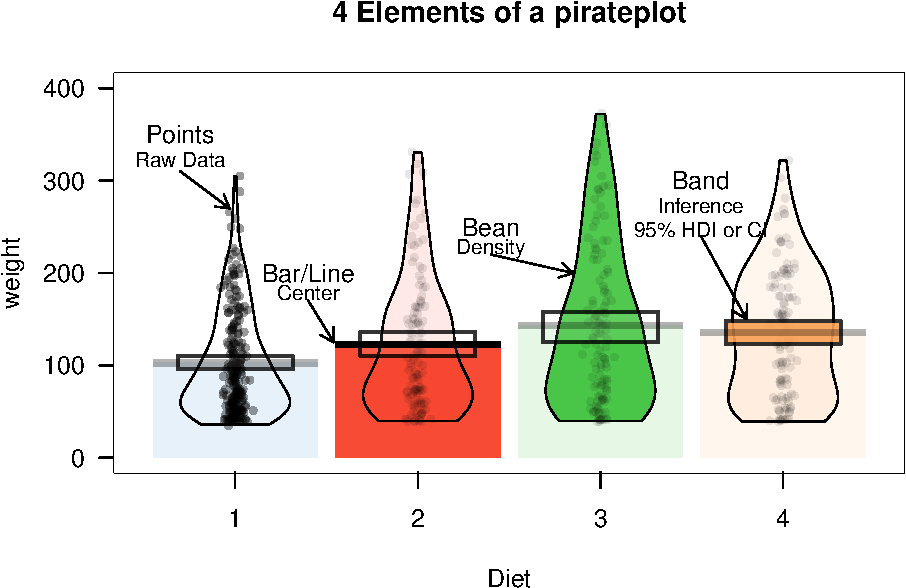
\includegraphics{YaRrr_files/figure-latex/pirateplot-1} 

}

\caption{The pirateplot(), an R pirate's favorite plot!}\label{fig:pirateplot}
\end{figure}

\begin{longtable}[]{@{}ll@{}}
\caption{\label{tab:pirateplotelements} 4 elements of a
\texttt{pirateplot()}}\tabularnewline
\toprule
\begin{minipage}[b]{0.18\columnwidth}\raggedright\strut
Element\strut
\end{minipage} & \begin{minipage}[b]{0.67\columnwidth}\raggedright\strut
Description\strut
\end{minipage}\tabularnewline
\midrule
\endfirsthead
\toprule
\begin{minipage}[b]{0.18\columnwidth}\raggedright\strut
Element\strut
\end{minipage} & \begin{minipage}[b]{0.67\columnwidth}\raggedright\strut
Description\strut
\end{minipage}\tabularnewline
\midrule
\endhead
\begin{minipage}[t]{0.18\columnwidth}\raggedright\strut
Points\strut
\end{minipage} & \begin{minipage}[t]{0.67\columnwidth}\raggedright\strut
\textbf{Raw} data.\strut
\end{minipage}\tabularnewline
\begin{minipage}[t]{0.18\columnwidth}\raggedright\strut
Bar / Line\strut
\end{minipage} & \begin{minipage}[t]{0.67\columnwidth}\raggedright\strut
\textbf{Descriptive} statistic, usually the mean or median\strut
\end{minipage}\tabularnewline
\begin{minipage}[t]{0.18\columnwidth}\raggedright\strut
Bean\strut
\end{minipage} & \begin{minipage}[t]{0.67\columnwidth}\raggedright\strut
Smoothed density curve showing the full data distribution.\strut
\end{minipage}\tabularnewline
\begin{minipage}[t]{0.18\columnwidth}\raggedright\strut
Band\strut
\end{minipage} & \begin{minipage}[t]{0.67\columnwidth}\raggedright\strut
\textbf{Inference} around the mean, either a Bayesian Highest Density
Interval (HDI), or a Confidence Interval (CI)\strut
\end{minipage}\tabularnewline
\bottomrule
\end{longtable}

The two main arguments to \texttt{pirateplot()} are \texttt{formula} and
\texttt{data}. In \texttt{formula}, you specify plotting variables in
the form \texttt{y\ \textasciitilde{}\ x}, where \texttt{y} is the name
of the dependent variable, and \texttt{x} is the name of the independent
variable. In \texttt{data}, you specify the name of the dataframe object
where the variables are stored.

Let's create a pirateplot of the ChickWeight data. I'll set the
dependent variable to \texttt{weight}, and the independent variable to
\texttt{Time} using the argument
\texttt{formula\ =\ weight\ \textasciitilde{}\ Time}:

\begin{Shaded}
\begin{Highlighting}[]
\NormalTok{yarrr::}\KeywordTok{pirateplot}\NormalTok{(}\DataTypeTok{formula =} \NormalTok{weight ~}\StringTok{ }\NormalTok{Time, }\CommentTok{# dv is weight, iv is Diet}
                   \DataTypeTok{data =} \NormalTok{ChickWeight,}
                   \DataTypeTok{main =} \StringTok{"Pirateplot of chicken weights"}\NormalTok{,}
                   \DataTypeTok{xlab =} \StringTok{"Diet"}\NormalTok{,}
                   \DataTypeTok{ylab =} \StringTok{"Weight"}\NormalTok{)}
\end{Highlighting}
\end{Shaded}

\begin{center}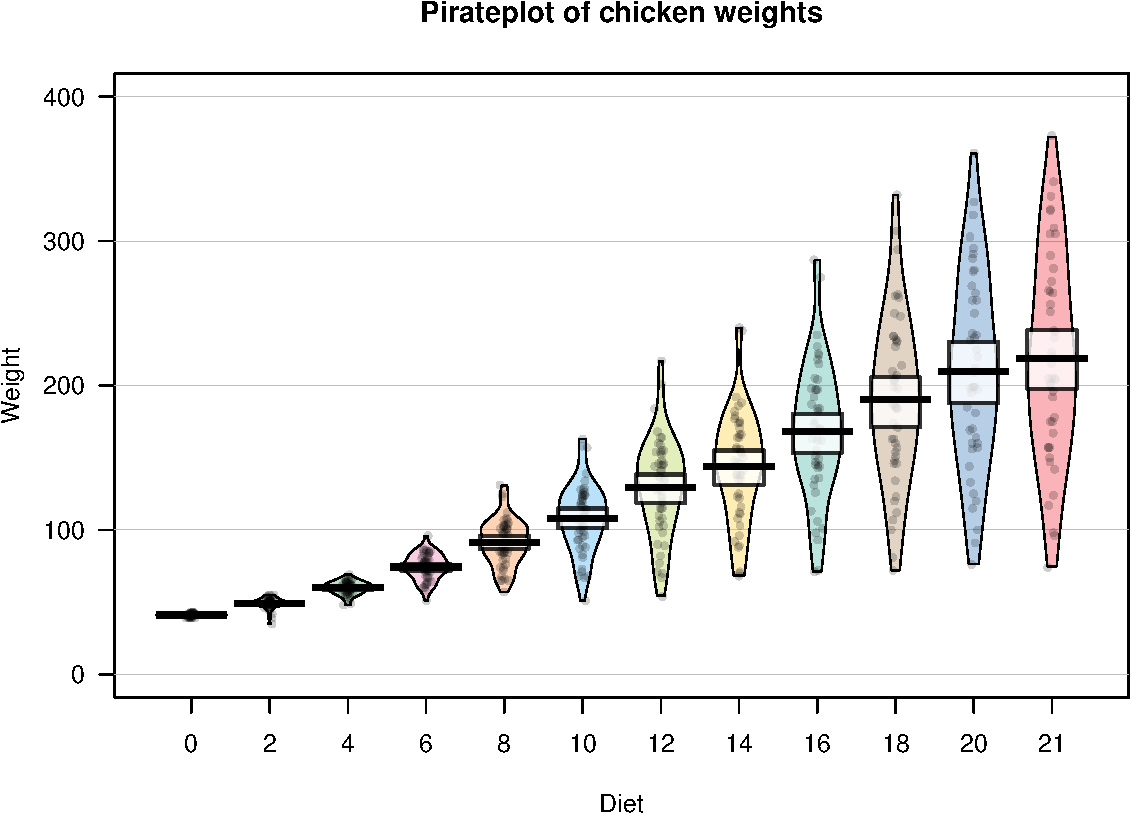
\includegraphics{YaRrr_files/figure-latex/chickpirateplot-1} \end{center}

\subsection{Pirateplot themes}\label{pirateplot-themes}

There are many different pirateplot themes, these themes dictate the
overall look of the plot. To specify a theme, just use the
\texttt{theme\ =\ x} argument, where \texttt{x} is the theme number:

\begin{center}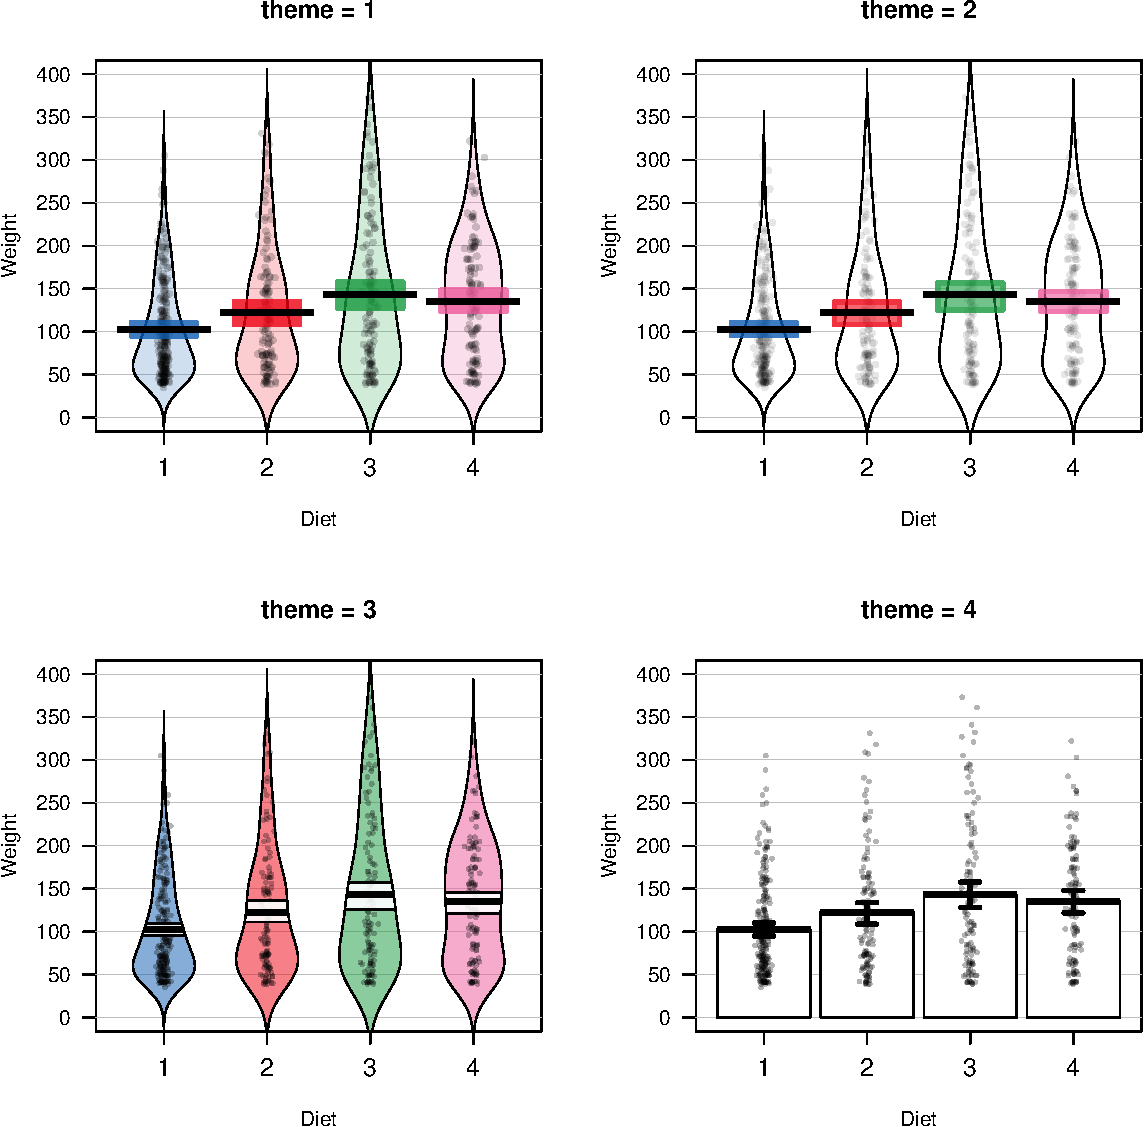
\includegraphics{YaRrr_files/figure-latex/unnamed-chunk-17-1} \end{center}

For example, here is a pirateplot height data from the \texttt{pirates}
dataframe using \texttt{theme\ =\ 3}. Here, I'll plot pirates' heights
as a function of their sex and whether or not they wear a headband. I'll
also make the plot all grayscale by using the \texttt{pal\ =\ "gray"}
argument:

\begin{Shaded}
\begin{Highlighting}[]
\NormalTok{yarrr::}\KeywordTok{pirateplot}\NormalTok{(}\DataTypeTok{formula =} \NormalTok{height ~}\StringTok{ }\NormalTok{sex +}\StringTok{ }\NormalTok{headband,    }\CommentTok{# DV = height, IV1 = sex, IV2 = headband}
                  \DataTypeTok{data =} \NormalTok{pirates,           }
                  \DataTypeTok{theme =} \DecValTok{3}\NormalTok{,}
                  \DataTypeTok{main =} \StringTok{"Pirate Heights"}\NormalTok{,}
                  \DataTypeTok{pal =} \StringTok{"gray"}\NormalTok{)}
\end{Highlighting}
\end{Shaded}

\begin{center}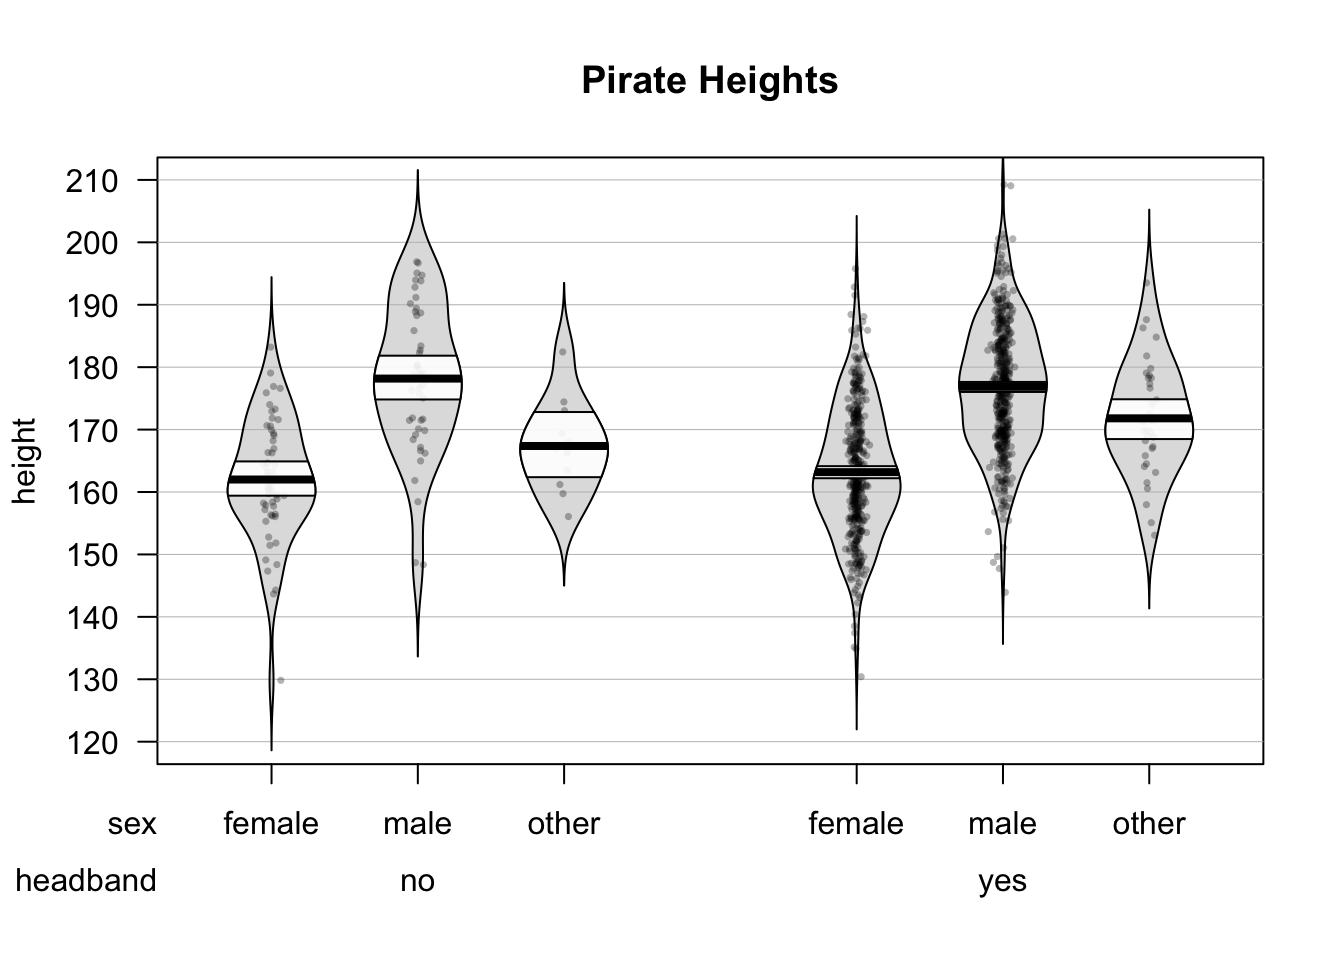
\includegraphics{YaRrr_files/figure-latex/unnamed-chunk-18-1} \end{center}

\subsection{Customizing pirateplots}\label{customizing-pirateplots}

Regardless of the theme you use, you can always customize the color and
opacity of graphical elements. To do this, specify one of the following
arguments. Note: Arguments with \texttt{.f.} correspond to the
\emph{filling} of an element, while \texttt{.b.} correspond to the
\emph{border} of an element:

\begin{table}

\caption{\label{tab:unnamed-chunk-19}Customising plotting elements}
\centering
\begin{tabular}[t]{l|l|l}
\hline
element & color & opacity\\
\hline
points & point.col, point.bg & point.o\\
\hline
beans & bean.f.col, bean.b.col & bean.f.o, bean.b.o\\
\hline
bar & bar.f.col, bar.b.col & bar.f.o, bar.b.o\\
\hline
inf & inf.f.col, inf.b.col & inf.f.o, inf.b.o\\
\hline
avg.line & avg.line.col & avg.line.o\\
\hline
\end{tabular}
\end{table}

For example, I could create the following pirateplots using
\texttt{theme\ =\ 0} and specifying elements explicitly:

\begin{Shaded}
\begin{Highlighting}[]
\KeywordTok{pirateplot}\NormalTok{(}\DataTypeTok{formula =} \NormalTok{weight ~}\StringTok{ }\NormalTok{Time,}
           \DataTypeTok{data =} \NormalTok{ChickWeight,}
           \DataTypeTok{theme =} \DecValTok{0}\NormalTok{,}
           \DataTypeTok{main =} \StringTok{"Fully customized pirateplot"}\NormalTok{,}
           \DataTypeTok{pal =} \StringTok{"southpark"}\NormalTok{, }\CommentTok{# southpark color palette}
           \DataTypeTok{bean.f.o =} \NormalTok{.}\DecValTok{6}\NormalTok{, }\CommentTok{# Bean fill}
           \DataTypeTok{point.o =} \NormalTok{.}\DecValTok{3}\NormalTok{, }\CommentTok{# Points}
           \DataTypeTok{inf.f.o =} \NormalTok{.}\DecValTok{7}\NormalTok{, }\CommentTok{# Inference fill}
           \DataTypeTok{inf.b.o =} \NormalTok{.}\DecValTok{8}\NormalTok{, }\CommentTok{# Inference border}
           \DataTypeTok{avg.line.o =} \DecValTok{1}\NormalTok{, }\CommentTok{# Average line}
           \DataTypeTok{bar.f.o =} \NormalTok{.}\DecValTok{5}\NormalTok{, }\CommentTok{# Bar}
           \DataTypeTok{inf.f.col =} \StringTok{"white"}\NormalTok{, }\CommentTok{# Inf fill col}
           \DataTypeTok{inf.b.col =} \StringTok{"black"}\NormalTok{, }\CommentTok{# Inf border col}
           \DataTypeTok{avg.line.col =} \StringTok{"black"}\NormalTok{, }\CommentTok{# avg line col}
           \DataTypeTok{bar.f.col =} \KeywordTok{gray}\NormalTok{(.}\DecValTok{8}\NormalTok{), }\CommentTok{# bar filling color}
           \DataTypeTok{point.pch =} \DecValTok{21}\NormalTok{,}
           \DataTypeTok{point.bg =} \StringTok{"white"}\NormalTok{,}
           \DataTypeTok{point.col =} \StringTok{"black"}\NormalTok{,}
           \DataTypeTok{point.cex =} \NormalTok{.}\DecValTok{7}\NormalTok{)}
\end{Highlighting}
\end{Shaded}

\begin{center}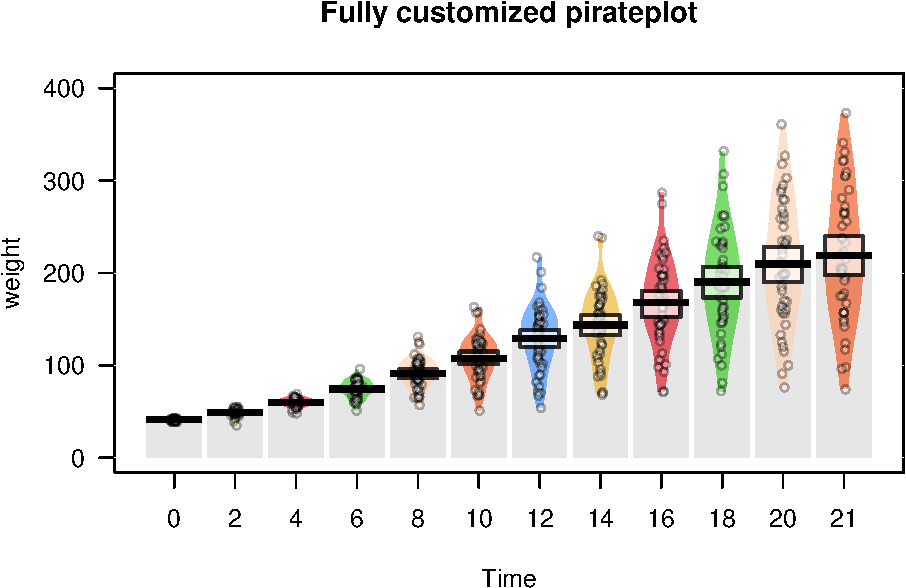
\includegraphics{YaRrr_files/figure-latex/unnamed-chunk-20-1} \end{center}

If you don't want to start from scratch, you can also start with a
theme, and then make selective adjustments:

\begin{Shaded}
\begin{Highlighting}[]
\KeywordTok{pirateplot}\NormalTok{(}\DataTypeTok{formula =} \NormalTok{weight ~}\StringTok{ }\NormalTok{Time,}
           \DataTypeTok{data =} \NormalTok{ChickWeight,}
           \DataTypeTok{main =} \StringTok{"Adjusting an existing theme"}\NormalTok{,}
           \DataTypeTok{theme =} \DecValTok{2}\NormalTok{,  }\CommentTok{# Start with theme 2}
           \DataTypeTok{inf.f.o =} \DecValTok{0}\NormalTok{, }\CommentTok{# Turn off inf fill}
           \DataTypeTok{inf.b.o =} \DecValTok{0}\NormalTok{, }\CommentTok{# Turn off inf border}
           \DataTypeTok{point.o =} \NormalTok{.}\DecValTok{2}\NormalTok{,   }\CommentTok{# Turn up points}
           \DataTypeTok{bar.f.o =} \NormalTok{.}\DecValTok{5}\NormalTok{, }\CommentTok{# Turn up bars}
           \DataTypeTok{bean.f.o =} \NormalTok{.}\DecValTok{4}\NormalTok{, }\CommentTok{# Light bean filling}
           \DataTypeTok{bean.b.o =} \NormalTok{.}\DecValTok{2}\NormalTok{, }\CommentTok{# Light bean border}
           \DataTypeTok{avg.line.o =} \DecValTok{0}\NormalTok{, }\CommentTok{# Turn off average line}
           \DataTypeTok{point.col =} \StringTok{"black"}\NormalTok{) }\CommentTok{# Black points}
\end{Highlighting}
\end{Shaded}

\begin{center}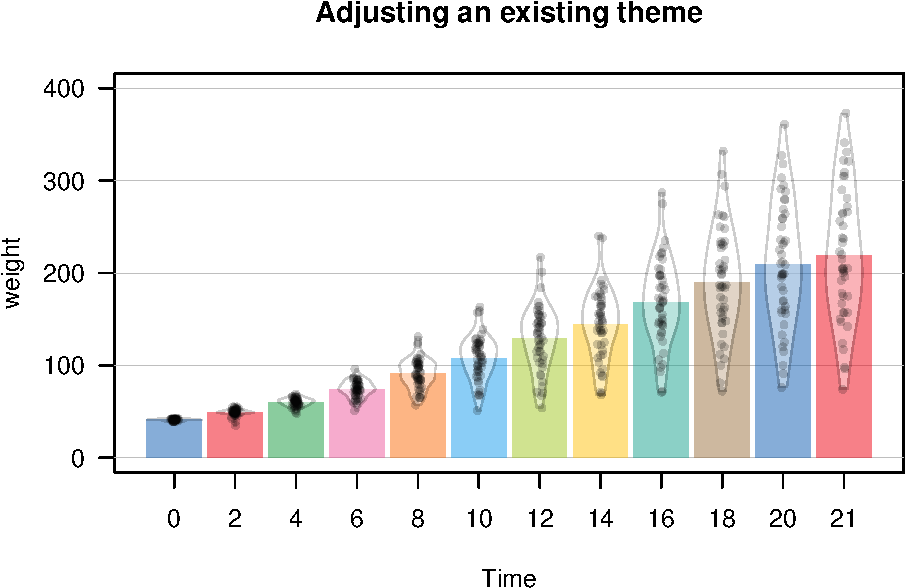
\includegraphics{YaRrr_files/figure-latex/unnamed-chunk-21-1} \end{center}

Just to drive the point home, as a barplot is a special case of a
pirateplot, you can even reduce a pirateplot into a horrible barplot:

\begin{Shaded}
\begin{Highlighting}[]
\CommentTok{# Reducing a pirateplot to a (at least colorful) barplot}
\KeywordTok{pirateplot}\NormalTok{(}\DataTypeTok{formula =} \NormalTok{weight ~}\StringTok{ }\NormalTok{Diet,}
           \DataTypeTok{data =} \NormalTok{ChickWeight,}
           \DataTypeTok{main =} \StringTok{"Reducing a pirateplot to a (horrible) barplot"}\NormalTok{,}
           \DataTypeTok{theme =} \DecValTok{0}\NormalTok{,                                    }\CommentTok{# Start from scratch}
           \DataTypeTok{pal =} \StringTok{"black"}\NormalTok{,}
           \DataTypeTok{inf.disp =} \StringTok{"line"}\NormalTok{,                            }\CommentTok{# Use a line for inference}
           \DataTypeTok{inf.f.o =} \DecValTok{1}\NormalTok{,                                  }\CommentTok{# Turn up inference opacity}
           \DataTypeTok{inf.f.col =} \StringTok{"black"}\NormalTok{,                          }\CommentTok{# Set inference line color}
           \DataTypeTok{bar.f.o =} \NormalTok{.}\DecValTok{3}\NormalTok{)                                }
\end{Highlighting}
\end{Shaded}

\begin{center}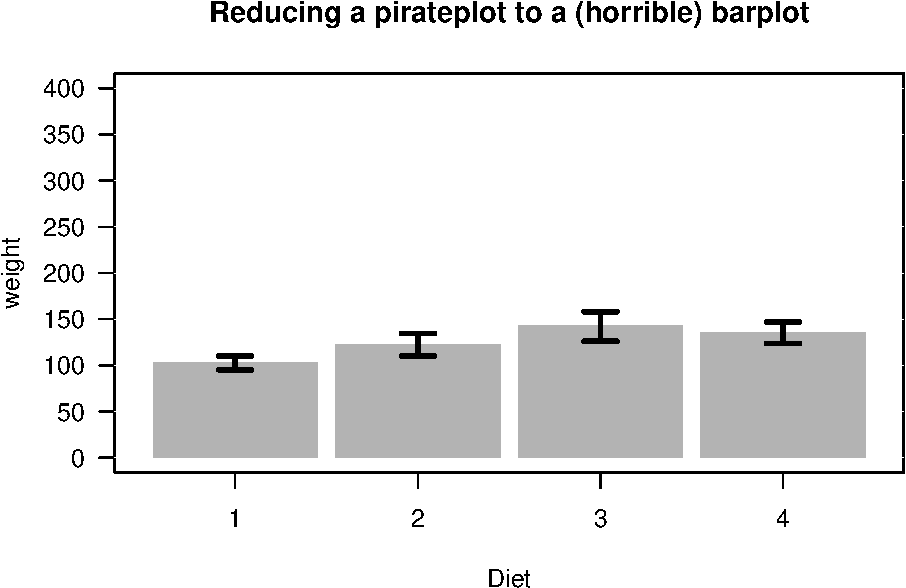
\includegraphics{YaRrr_files/figure-latex/unnamed-chunk-22-1} \end{center}

There are many additional arguments to \texttt{pirateplot()} that you
can use to complete customize the look of your plot. To see them all,
look at the help menu with \texttt{?pirateplot} or look at the vignette
at \href{}{}

\begin{longtable}[]{@{}lll@{}}
\caption{\label{tab:pirateplotcustomisation} Additional
\texttt{pirateplot()} customizations.}\tabularnewline
\toprule
\begin{minipage}[b]{0.19\columnwidth}\raggedright\strut
Element\strut
\end{minipage} & \begin{minipage}[b]{0.24\columnwidth}\raggedright\strut
Argument\strut
\end{minipage} & \begin{minipage}[b]{0.48\columnwidth}\raggedright\strut
Examples\strut
\end{minipage}\tabularnewline
\midrule
\endfirsthead
\toprule
\begin{minipage}[b]{0.19\columnwidth}\raggedright\strut
Element\strut
\end{minipage} & \begin{minipage}[b]{0.24\columnwidth}\raggedright\strut
Argument\strut
\end{minipage} & \begin{minipage}[b]{0.48\columnwidth}\raggedright\strut
Examples\strut
\end{minipage}\tabularnewline
\midrule
\endhead
\begin{minipage}[t]{0.19\columnwidth}\raggedright\strut
Background color\strut
\end{minipage} & \begin{minipage}[t]{0.24\columnwidth}\raggedright\strut
back.col\strut
\end{minipage} & \begin{minipage}[t]{0.48\columnwidth}\raggedright\strut
\texttt{back.col\ =\ \textquotesingle{}gray(.9,\ .9)\textquotesingle{}}\strut
\end{minipage}\tabularnewline
\begin{minipage}[t]{0.19\columnwidth}\raggedright\strut
Gridlines\strut
\end{minipage} & \begin{minipage}[t]{0.24\columnwidth}\raggedright\strut
gl.col, gl.lwd, gl.lty\strut
\end{minipage} & \begin{minipage}[t]{0.48\columnwidth}\raggedright\strut
\texttt{gl.col\ =\ \textquotesingle{}gray\textquotesingle{},\ gl.lwd\ =\ c(.75,\ 0),\ gl.lty\ =\ 1}\strut
\end{minipage}\tabularnewline
\begin{minipage}[t]{0.19\columnwidth}\raggedright\strut
Quantiles\strut
\end{minipage} & \begin{minipage}[t]{0.24\columnwidth}\raggedright\strut
quant, quant.lwd, quant.col\strut
\end{minipage} & \begin{minipage}[t]{0.48\columnwidth}\raggedright\strut
\texttt{quant\ =\ c(.1,\ .9),\ quant.lwd\ =\ 1,\ quant.col\ =\ \textquotesingle{}black\textquotesingle{}}\strut
\end{minipage}\tabularnewline
\begin{minipage}[t]{0.19\columnwidth}\raggedright\strut
Average line\strut
\end{minipage} & \begin{minipage}[t]{0.24\columnwidth}\raggedright\strut
avg.line.fun\strut
\end{minipage} & \begin{minipage}[t]{0.48\columnwidth}\raggedright\strut
\texttt{avg.line.fun\ =\ median}\strut
\end{minipage}\tabularnewline
\begin{minipage}[t]{0.19\columnwidth}\raggedright\strut
Inference Calculation\strut
\end{minipage} & \begin{minipage}[t]{0.24\columnwidth}\raggedright\strut
inf.method\strut
\end{minipage} & \begin{minipage}[t]{0.48\columnwidth}\raggedright\strut
\texttt{inf.method\ =\ \textquotesingle{}hdi\textquotesingle{}},
\texttt{inf.method\ =\ \textquotesingle{}ci\textquotesingle{}}\strut
\end{minipage}\tabularnewline
\begin{minipage}[t]{0.19\columnwidth}\raggedright\strut
Inference Display\strut
\end{minipage} & \begin{minipage}[t]{0.24\columnwidth}\raggedright\strut
inf.disp\strut
\end{minipage} & \begin{minipage}[t]{0.48\columnwidth}\raggedright\strut
\texttt{inf.disp\ =\ \textquotesingle{}line\textquotesingle{}},
\texttt{inf.disp\ =\ \textquotesingle{}bean\textquotesingle{}},
\texttt{inf.disp\ =\ \textquotesingle{}rect\textquotesingle{}}\strut
\end{minipage}\tabularnewline
\bottomrule
\end{longtable}

\begin{Shaded}
\begin{Highlighting}[]
\CommentTok{# Additional pirateplot customizations}
\KeywordTok{pirateplot}\NormalTok{(}\DataTypeTok{formula =} \NormalTok{weight ~}\StringTok{ }\NormalTok{Diet, }
           \DataTypeTok{data =} \NormalTok{ChickWeight,}
           \DataTypeTok{main =} \StringTok{"Adding quantile lines and background colors"}\NormalTok{,}
           \DataTypeTok{theme =} \DecValTok{2}\NormalTok{,}
           \DataTypeTok{cap.beans =} \OtherTok{TRUE}\NormalTok{,}
           \DataTypeTok{back.col =} \KeywordTok{transparent}\NormalTok{(}\StringTok{"blue"}\NormalTok{, .}\DecValTok{95}\NormalTok{), }\CommentTok{# Add light blue background}
           \DataTypeTok{gl.col =} \StringTok{"gray"}\NormalTok{, }\CommentTok{# Gray gridlines}
           \DataTypeTok{gl.lwd =} \KeywordTok{c}\NormalTok{(.}\DecValTok{75}\NormalTok{, }\DecValTok{0}\NormalTok{),}
           \DataTypeTok{inf.f.o =} \NormalTok{.}\DecValTok{6}\NormalTok{, }\CommentTok{# Turn up inf filling}
           \DataTypeTok{inf.disp =} \StringTok{"bean"}\NormalTok{, }\CommentTok{# Wrap inference around bean}
           \DataTypeTok{bean.b.o =} \NormalTok{.}\DecValTok{4}\NormalTok{, }\CommentTok{# Turn down bean borders}
           \DataTypeTok{quant =} \KeywordTok{c}\NormalTok{(.}\DecValTok{1}\NormalTok{, .}\DecValTok{9}\NormalTok{), }\CommentTok{# 10th and 90th quantiles}
           \DataTypeTok{quant.col =} \StringTok{"black"}\NormalTok{) }\CommentTok{# Black quantile lines}
\end{Highlighting}
\end{Shaded}

\begin{center}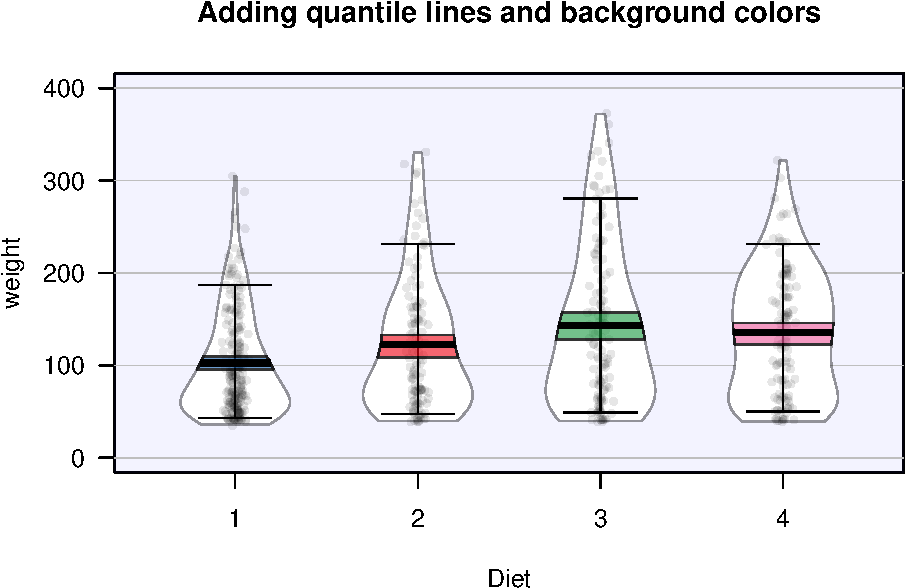
\includegraphics{YaRrr_files/figure-latex/unnamed-chunk-23-1} \end{center}

\subsection{Saving output}\label{saving-output}

If you include the \texttt{plot\ =\ FALSE} argument to a pirateplot, the
function will return some values associated with each bean in the plot.
In the next chunk, I'll

\begin{Shaded}
\begin{Highlighting}[]
\CommentTok{# Create a pirateplot}
\KeywordTok{pirateplot}\NormalTok{(}\DataTypeTok{formula =} \NormalTok{tattoos ~}\StringTok{ }\NormalTok{sex +}\StringTok{ }\NormalTok{headband,}
           \DataTypeTok{data =} \NormalTok{pirates)}
\end{Highlighting}
\end{Shaded}

\begin{center}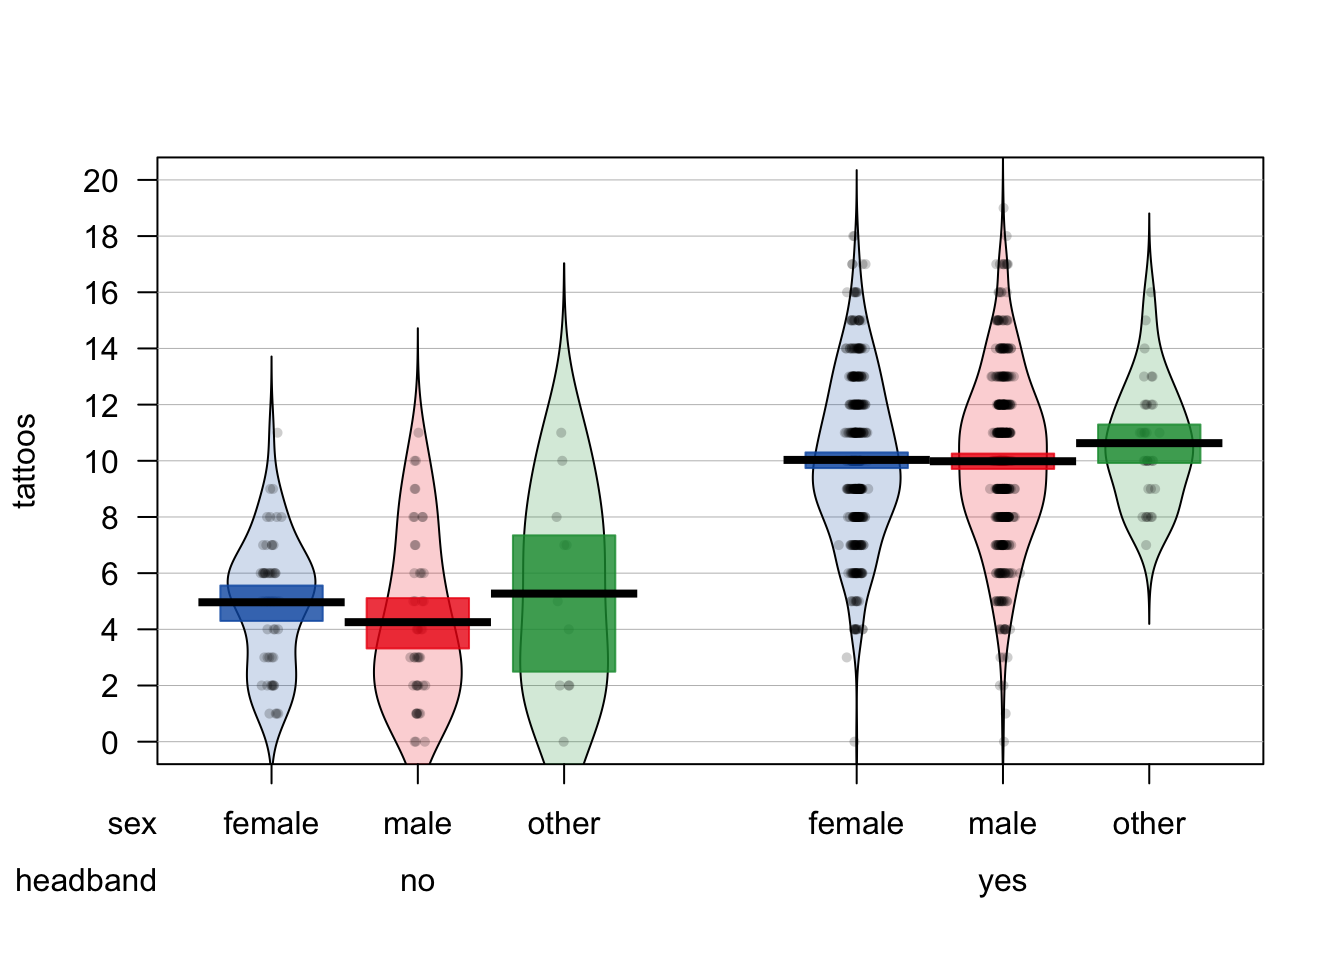
\includegraphics{YaRrr_files/figure-latex/unnamed-chunk-24-1} \end{center}

\begin{Shaded}
\begin{Highlighting}[]

\CommentTok{# Save data from the pirateplot to an object}
\NormalTok{tattoos.pp <-}\StringTok{ }\KeywordTok{pirateplot}\NormalTok{(}\DataTypeTok{formula =} \NormalTok{tattoos ~}\StringTok{ }\NormalTok{sex +}\StringTok{ }\NormalTok{headband,}
                         \DataTypeTok{data =} \NormalTok{pirates,}
                         \DataTypeTok{plot =} \OtherTok{FALSE}\NormalTok{)}
\end{Highlighting}
\end{Shaded}

Now I can access the summary and inferential statistics from the plot in
the \texttt{tattoos.pp} object. The most interesting element is
\texttt{\$summary} which shows summary statistics for each bean (aka,
group):

\begin{Shaded}
\begin{Highlighting}[]
\CommentTok{# Show me statistics from groups in the pirateplot}
\NormalTok{tattoos.pp}
\NormalTok{## $summary}
\NormalTok{##      sex headband bean.num   n       avg   inf.lb    inf.ub}
\NormalTok{## 1 female       no        1  55  4.963636 4.274457  5.491925}
\NormalTok{## 2   male       no        2  47  4.255319 3.230407  4.975205}
\NormalTok{## 3  other       no        3  11  5.272727 2.511369  7.207242}
\NormalTok{## 4 female      yes        4 409 10.031785 9.769694 10.318491}
\NormalTok{## 5   male      yes        5 443  9.984199 9.694375 10.268986}
\NormalTok{## 6  other      yes        6  35 10.628571 9.874442 11.350058}
\NormalTok{## }
\NormalTok{## $avg.line.fun}
\NormalTok{## [1] "mean"}
\NormalTok{## }
\NormalTok{## $inf.method}
\NormalTok{## [1] "hdi"}
\NormalTok{## }
\NormalTok{## $inf.p}
\NormalTok{## [1] 0.95}
\end{Highlighting}
\end{Shaded}

Once you've created a plot with a high-level plotting function, you can
add additional elements with \emph{low-level} functions. For example,
you can add data points with \texttt{points()}, reference lines with
\texttt{abline()}, text with \texttt{text()}, and legends with
\texttt{legend()}.

\section{Low-level plotting
functions}\label{low-level-plotting-functions}

Low-level plotting functions allow you to add elements, like points, or
lines, to an existing plot. Here are the most common low-level plotting
functions:

\begin{longtable}[]{@{}ll@{}}
\caption{\label{tab:lowlevelplotting} Common low-level plotting
functions.}\tabularnewline
\toprule
Function & Outcome\tabularnewline
\midrule
\endfirsthead
\toprule
Function & Outcome\tabularnewline
\midrule
\endhead
\texttt{points(x,\ y)} & Adds points\tabularnewline
\texttt{abline()}, \texttt{segments()} & Adds lines or
segments\tabularnewline
\texttt{arrows()} & Adds arrows\tabularnewline
\texttt{curve()} & Adds a curve representing a function\tabularnewline
\texttt{rect()},\texttt{polygon()} & Adds a rectangle or arbitrary
shape\tabularnewline
\texttt{text()}, \texttt{mtext()} & Adds text within the plot, or to
plot margins\tabularnewline
\texttt{legend()} & Adds a legend\tabularnewline
\texttt{axis()} & Adds an axis\tabularnewline
\bottomrule
\end{longtable}

\subsection{Starting with a blank
plot}\label{starting-with-a-blank-plot}

\begin{figure}

{\centering 
\includegraphics[width=0.75\linewidth]{images/canvas} 

}

\caption{Sometimes it's nice to start with a blank plotting canvas, and then add each element individually with low-level plotting commands}\label{fig:canvas}
\end{figure}

Before you start adding elements with low-level plotting functions, it's
useful to start with a blank plotting space like the one I have in
Figure \ref{fig:blankplot}. To do this, execute the \texttt{plot()}
function, but use the \texttt{type\ =\ "n"} argument to tell R that you
don't want to plot anything yet. Once you've created a blank plot, you
can additional elements with low-level plotting commands.

\begin{Shaded}
\begin{Highlighting}[]
\CommentTok{# Create a blank plotting space}
\KeywordTok{plot}\NormalTok{(}\DataTypeTok{x =} \DecValTok{1}\NormalTok{,                 }
     \DataTypeTok{xlab =} \StringTok{"X Label"}\NormalTok{, }
     \DataTypeTok{ylab =} \StringTok{"Y Label"}\NormalTok{,}
     \DataTypeTok{xlim =} \KeywordTok{c}\NormalTok{(}\DecValTok{0}\NormalTok{, }\DecValTok{100}\NormalTok{), }
     \DataTypeTok{ylim =} \KeywordTok{c}\NormalTok{(}\DecValTok{0}\NormalTok{, }\DecValTok{100}\NormalTok{),}
     \DataTypeTok{main =} \StringTok{"Blank Plotting Canvas"}\NormalTok{,}
     \DataTypeTok{type =} \StringTok{"n"}\NormalTok{)}
\end{Highlighting}
\end{Shaded}

\begin{figure}

{\centering 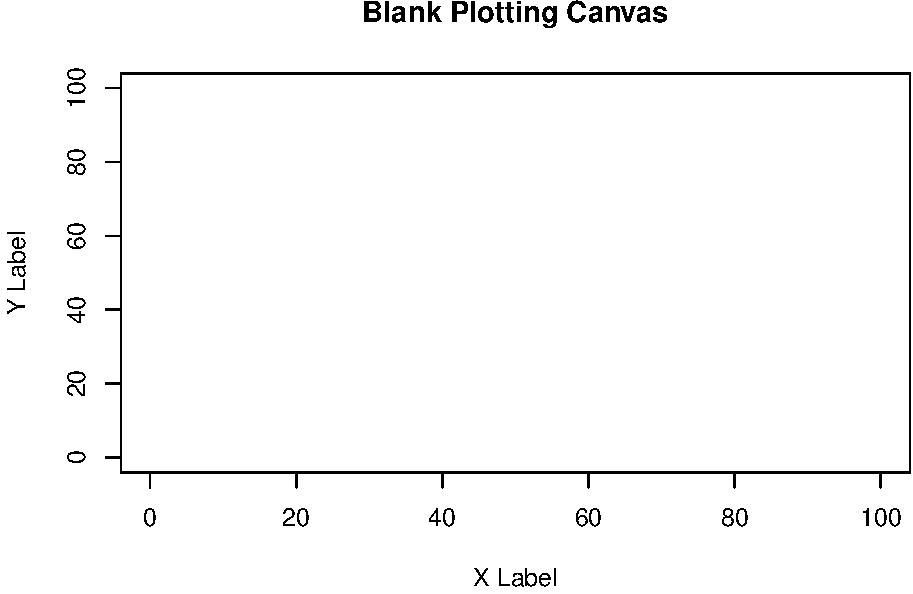
\includegraphics{YaRrr_files/figure-latex/blankplot-1} 

}

\caption{A blank plotting space, ready for additional elements!}\label{fig:blankplot}
\end{figure}

\subsection{\texorpdfstring{\texttt{points()}}{points()}}\label{points}

To add new points to an existing plot, use the \texttt{points()}
function. The \texttt{points} function has many similar arguments to the
\texttt{plot()} function, like \texttt{x} (for the x-coordinates),
\texttt{y} (for the y-coordinates), and parameters like \texttt{col}
(border color), \texttt{cex} (point size), and \texttt{pch} (symbol
type). To see all of them, look at the help menu with
\texttt{?points()}.

Let's use \texttt{points()} to create a plot with different symbol types
for different data. I'll use the pirates dataset and plot the
relationship between a pirate's age and the number of tattoos he/she
has. I'll create separate points for male and female pirates:

\begin{Shaded}
\begin{Highlighting}[]
\CommentTok{# Create a blank plot}
\KeywordTok{plot}\NormalTok{(}\DataTypeTok{x =} \DecValTok{1}\NormalTok{,}
     \DataTypeTok{type =} \StringTok{"n"}\NormalTok{,}
     \DataTypeTok{xlim =} \KeywordTok{c}\NormalTok{(}\DecValTok{100}\NormalTok{, }\DecValTok{225}\NormalTok{), }
     \DataTypeTok{ylim =} \KeywordTok{c}\NormalTok{(}\DecValTok{30}\NormalTok{, }\DecValTok{110}\NormalTok{),}
     \DataTypeTok{pch =} \DecValTok{16}\NormalTok{,}
     \DataTypeTok{xlab =} \StringTok{"Height"}\NormalTok{, }
     \DataTypeTok{ylab =} \StringTok{"Weight"}\NormalTok{,}
     \DataTypeTok{main =} \StringTok{"Adding points to a plot with points()"}\NormalTok{)}

\CommentTok{# Add coral2 points for male data}
\KeywordTok{points}\NormalTok{(}\DataTypeTok{x =} \NormalTok{pirates$height[pirates$sex ==}\StringTok{ "male"}\NormalTok{],}
       \DataTypeTok{y =} \NormalTok{pirates$weight[pirates$sex ==}\StringTok{ "male"}\NormalTok{],}
       \DataTypeTok{pch =} \DecValTok{16}\NormalTok{,}
       \DataTypeTok{col =} \KeywordTok{transparent}\NormalTok{(}\StringTok{"coral2"}\NormalTok{, }\DataTypeTok{trans.val =} \NormalTok{.}\DecValTok{8}\NormalTok{))}

\CommentTok{# Add steelblue points for female data}
\KeywordTok{points}\NormalTok{(}\DataTypeTok{x =} \NormalTok{pirates$height[pirates$sex ==}\StringTok{ "female"}\NormalTok{],}
       \DataTypeTok{y =} \NormalTok{pirates$weight[pirates$sex ==}\StringTok{ "female"}\NormalTok{],}
       \DataTypeTok{pch =} \DecValTok{16}\NormalTok{,}
       \DataTypeTok{col =} \KeywordTok{transparent}\NormalTok{(}\StringTok{"steelblue3"}\NormalTok{, }\DataTypeTok{trans.val =} \NormalTok{.}\DecValTok{8}\NormalTok{))}
\end{Highlighting}
\end{Shaded}

\begin{figure}

{\centering 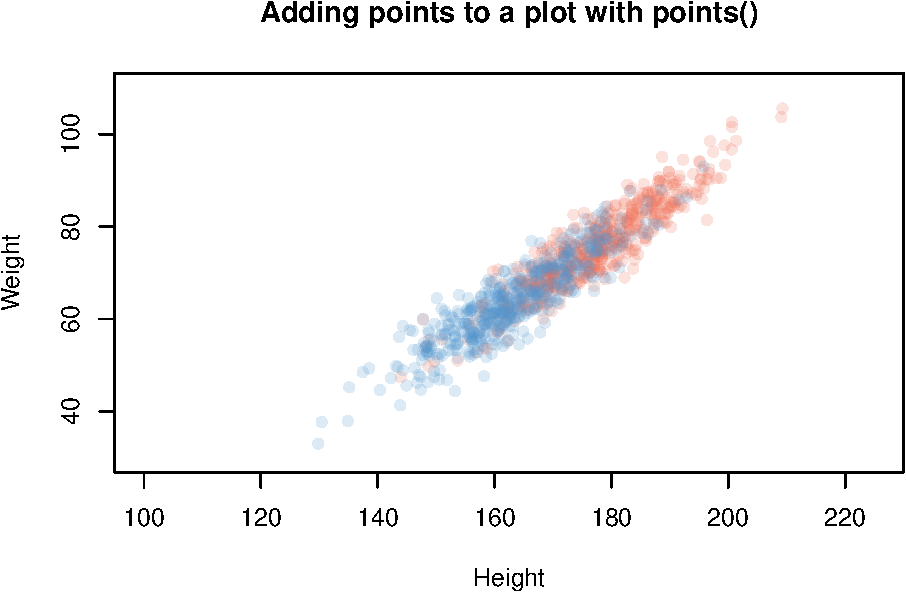
\includegraphics{YaRrr_files/figure-latex/pointsexample-1} 

}

\caption{Using points() to add points with different colors}\label{fig:pointsexample}
\end{figure}

\subsection{\texorpdfstring{\texttt{abline()}, \texttt{segments()},
\texttt{grid()}}{abline(), segments(), grid()}}\label{abline-segments-grid}

\begin{longtable}[]{@{}ll@{}}
\caption{\label{tab:linearguments} Arguments to \texttt{abline()} and
\texttt{segments()}}\tabularnewline
\toprule
\begin{minipage}[b]{0.14\columnwidth}\raggedright\strut
Argument\strut
\end{minipage} & \begin{minipage}[b]{0.50\columnwidth}\raggedright\strut
Outcome\strut
\end{minipage}\tabularnewline
\midrule
\endfirsthead
\toprule
\begin{minipage}[b]{0.14\columnwidth}\raggedright\strut
Argument\strut
\end{minipage} & \begin{minipage}[b]{0.50\columnwidth}\raggedright\strut
Outcome\strut
\end{minipage}\tabularnewline
\midrule
\endhead
\begin{minipage}[t]{0.14\columnwidth}\raggedright\strut
\texttt{h,\ v}\strut
\end{minipage} & \begin{minipage}[t]{0.50\columnwidth}\raggedright\strut
Locations of horizontal and vertical lines (for \texttt{abline()}
only)\strut
\end{minipage}\tabularnewline
\begin{minipage}[t]{0.14\columnwidth}\raggedright\strut
\texttt{x0,\ y0,\ x1,\ y1}\strut
\end{minipage} & \begin{minipage}[t]{0.50\columnwidth}\raggedright\strut
Starting and ending coordinates of lines (for \texttt{segments()}
only)\strut
\end{minipage}\tabularnewline
\begin{minipage}[t]{0.14\columnwidth}\raggedright\strut
\texttt{lty}\strut
\end{minipage} & \begin{minipage}[t]{0.50\columnwidth}\raggedright\strut
Line type. 1 = solid, 2 = dashed, 3 = dotted, \ldots{}\strut
\end{minipage}\tabularnewline
\begin{minipage}[t]{0.14\columnwidth}\raggedright\strut
\texttt{lwd}\strut
\end{minipage} & \begin{minipage}[t]{0.50\columnwidth}\raggedright\strut
Width of the lines specified by a number. 1 is the default (.2 is very
thin, 5 is very thick)\strut
\end{minipage}\tabularnewline
\begin{minipage}[t]{0.14\columnwidth}\raggedright\strut
\texttt{col}\strut
\end{minipage} & \begin{minipage}[t]{0.50\columnwidth}\raggedright\strut
Line color\strut
\end{minipage}\tabularnewline
\bottomrule
\end{longtable}

To add straight lines to a plot, use \texttt{abline()} or
\texttt{segments()}. \texttt{abline()} will add a line across the entire
plot, while \texttt{segments()} will add a line with defined starting
and end points.

For example, we can add reference lines to a plot with
\texttt{abline()}. In the following plot, I'll add vertical and
horizontal reference lines showing the means of the variables on the x
and y axes, for the horizontal line, I'll specify
\texttt{h\ =\ mean(pirates\$height)}, for the vertical line, I'll
specify \texttt{v\ =\ mean(pirates\$weight)}

\begin{Shaded}
\begin{Highlighting}[]
\KeywordTok{plot}\NormalTok{(}\DataTypeTok{x =} \NormalTok{pirates$weight,}
     \DataTypeTok{y =} \NormalTok{pirates$height,}
     \DataTypeTok{xlab =} \StringTok{"weight"}\NormalTok{,}
     \DataTypeTok{ylab =} \StringTok{"height"}\NormalTok{,}
     \DataTypeTok{main =} \StringTok{"Adding reference lines with abline"}\NormalTok{, }
     \DataTypeTok{pch =} \DecValTok{16}\NormalTok{, }
     \DataTypeTok{col =} \KeywordTok{gray}\NormalTok{(.}\DecValTok{5}\NormalTok{, .}\DecValTok{2}\NormalTok{))}

\CommentTok{# Add horizontal line at mean height}
\KeywordTok{abline}\NormalTok{(}\DataTypeTok{h =} \KeywordTok{mean}\NormalTok{(pirates$height), }
       \DataTypeTok{lty =} \DecValTok{2}\NormalTok{)                        }\CommentTok{# Dashed line}

\CommentTok{# Add vertical line at mean weight}
\KeywordTok{abline}\NormalTok{(}\DataTypeTok{v =} \KeywordTok{mean}\NormalTok{(pirates$weight),}
       \DataTypeTok{lty =} \DecValTok{2}\NormalTok{)                        }\CommentTok{# Dashed line}
\end{Highlighting}
\end{Shaded}

\begin{center}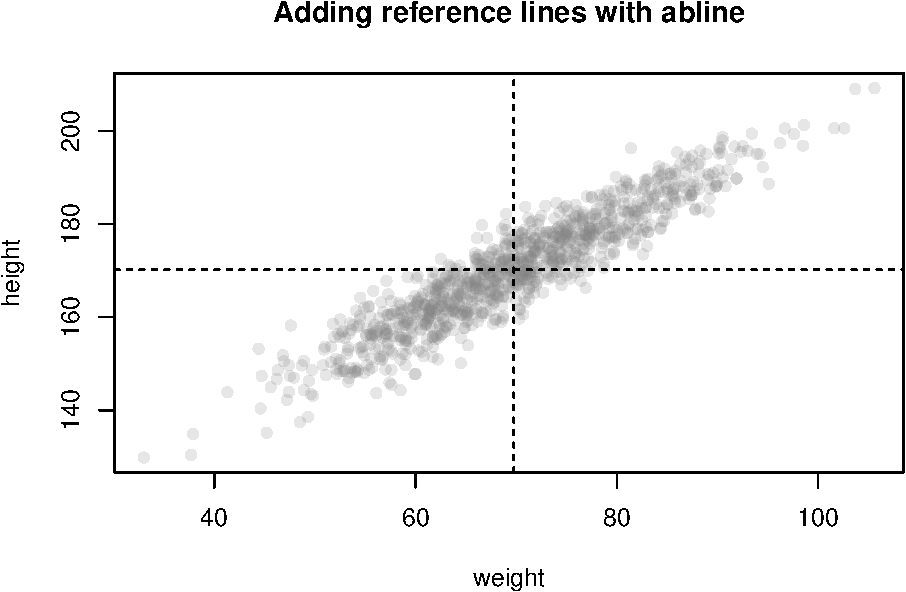
\includegraphics{YaRrr_files/figure-latex/unnamed-chunk-26-1} \end{center}

To change the look of your lines, use the \texttt{lty} argument, which
changes the type of line (see Figure \ref{fig:ltytypes}), \texttt{lwd},
which changes its thickness, and \texttt{col} which changes its color

\begin{figure}

{\centering 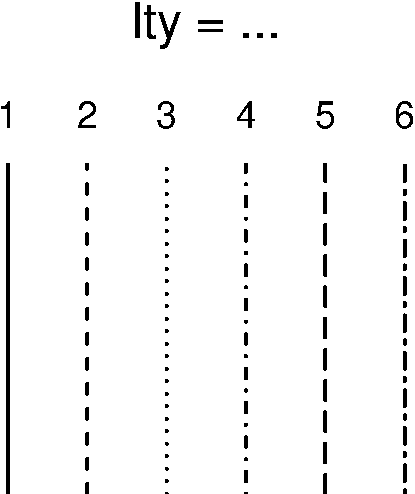
\includegraphics{YaRrr_files/figure-latex/ltytypes-1} 

}

\caption{Changing line type with the lty argument.}\label{fig:ltytypes}
\end{figure}

You can also add a regression line (also called a line of best fit) to a
scatterplot by entering a regression object created with \texttt{lm()}
as the main argument to \texttt{abline()}:

\begin{Shaded}
\begin{Highlighting}[]
\CommentTok{# Add a regression line to a scatterplot}
\KeywordTok{plot}\NormalTok{(}\DataTypeTok{x =} \NormalTok{pirates$height,}
     \DataTypeTok{y =} \NormalTok{pirates$weight,}
     \DataTypeTok{pch =} \DecValTok{16}\NormalTok{,}
     \DataTypeTok{col =} \KeywordTok{transparent}\NormalTok{(}\StringTok{"purple"}\NormalTok{, .}\DecValTok{7}\NormalTok{),}
     \DataTypeTok{main =} \StringTok{"Adding a regression line to a scatterplot()"}\NormalTok{)}

\CommentTok{# Add the regression line}
\KeywordTok{abline}\NormalTok{(}\KeywordTok{lm}\NormalTok{(weight ~}\StringTok{ }\NormalTok{height, }\DataTypeTok{data =} \NormalTok{pirates), }
       \DataTypeTok{lty =} \DecValTok{2}\NormalTok{)}
\end{Highlighting}
\end{Shaded}

\begin{center}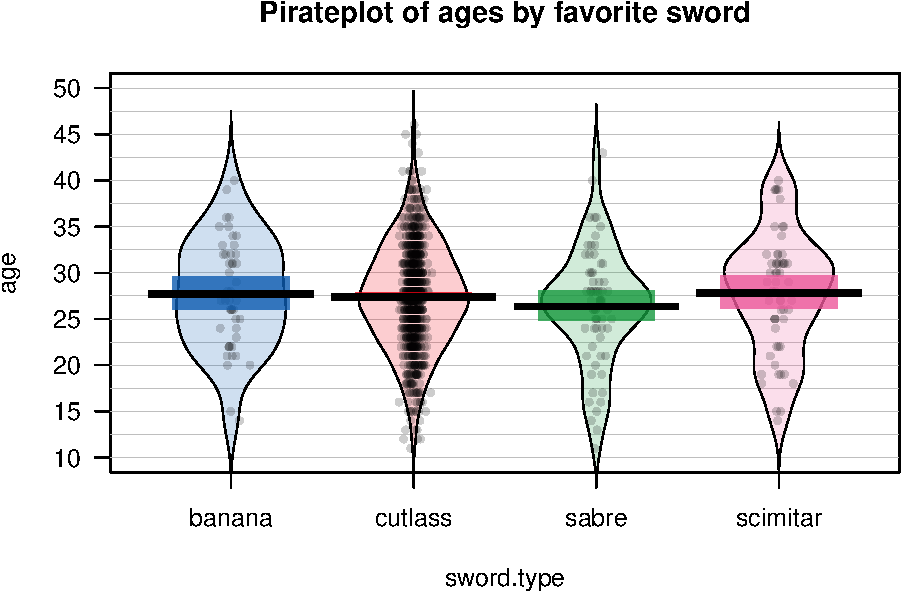
\includegraphics{YaRrr_files/figure-latex/unnamed-chunk-27-1} \end{center}

The \texttt{segments()} function works very similarly to
\texttt{abline()} -- however, with the \texttt{segments()} function, you
specify the beginning and end points of the segments with the arguments
\texttt{x0}, \texttt{y0}, \texttt{x1}, and \texttt{y1}. In Figure
\ref{fig:segments} I use \texttt{segments()} to connect two vectors of
data:

\begin{Shaded}
\begin{Highlighting}[]
\CommentTok{# Before and after data}
\NormalTok{before <-}\StringTok{ }\KeywordTok{c}\NormalTok{(}\FloatTok{2.1}\NormalTok{, }\FloatTok{3.5}\NormalTok{, }\FloatTok{1.8}\NormalTok{, }\FloatTok{4.2}\NormalTok{, }\FloatTok{2.4}\NormalTok{, }\FloatTok{3.9}\NormalTok{, }\FloatTok{2.1}\NormalTok{, }\FloatTok{4.4}\NormalTok{)}
\NormalTok{after <-}\StringTok{ }\KeywordTok{c}\NormalTok{(}\FloatTok{7.5}\NormalTok{, }\FloatTok{5.1}\NormalTok{, }\FloatTok{6.9}\NormalTok{, }\FloatTok{3.6}\NormalTok{, }\FloatTok{7.5}\NormalTok{, }\FloatTok{5.2}\NormalTok{, }\FloatTok{6.1}\NormalTok{, }\FloatTok{7.3}\NormalTok{)}

\CommentTok{# Create plotting space and before scores}
\KeywordTok{plot}\NormalTok{(}\DataTypeTok{x =} \KeywordTok{rep}\NormalTok{(}\DecValTok{1}\NormalTok{, }\KeywordTok{length}\NormalTok{(before)), }
     \DataTypeTok{y =} \NormalTok{before, }
     \DataTypeTok{xlim =} \KeywordTok{c}\NormalTok{(.}\DecValTok{5}\NormalTok{, }\FloatTok{2.5}\NormalTok{), }
     \DataTypeTok{ylim =} \KeywordTok{c}\NormalTok{(}\DecValTok{0}\NormalTok{, }\DecValTok{11}\NormalTok{),}
     \DataTypeTok{ylab =} \StringTok{"Score"}\NormalTok{, }
     \DataTypeTok{xlab =} \StringTok{"Time"}\NormalTok{,}
     \DataTypeTok{main =} \StringTok{"Using segments() to connect points"}\NormalTok{, }
     \DataTypeTok{xaxt =} \StringTok{"n"}\NormalTok{)}

\CommentTok{# Add after scores}
\KeywordTok{points}\NormalTok{(}\DataTypeTok{x =} \KeywordTok{rep}\NormalTok{(}\DecValTok{2}\NormalTok{, }\KeywordTok{length}\NormalTok{(after)), }\DataTypeTok{y =} \NormalTok{after)}

\CommentTok{# Add connections with segments()}
\KeywordTok{segments}\NormalTok{(}\DataTypeTok{x0 =} \KeywordTok{rep}\NormalTok{(}\DecValTok{1}\NormalTok{, }\KeywordTok{length}\NormalTok{(before)), }
         \DataTypeTok{y0 =} \NormalTok{before, }
         \DataTypeTok{x1 =} \KeywordTok{rep}\NormalTok{(}\DecValTok{2}\NormalTok{, }\KeywordTok{length}\NormalTok{(after)), }
         \DataTypeTok{y1 =} \NormalTok{after, }
         \DataTypeTok{col =} \KeywordTok{gray}\NormalTok{(}\DecValTok{0}\NormalTok{, .}\DecValTok{5}\NormalTok{))}

\CommentTok{# Add labels}
\KeywordTok{mtext}\NormalTok{(}\DataTypeTok{text =} \KeywordTok{c}\NormalTok{(}\StringTok{"Before"}\NormalTok{, }\StringTok{"After"}\NormalTok{), }
      \DataTypeTok{side =} \DecValTok{1}\NormalTok{, }\DataTypeTok{at =} \KeywordTok{c}\NormalTok{(}\DecValTok{1}\NormalTok{, }\DecValTok{2}\NormalTok{), }\DataTypeTok{line =} \DecValTok{1}\NormalTok{)}
\end{Highlighting}
\end{Shaded}

\begin{figure}

{\centering 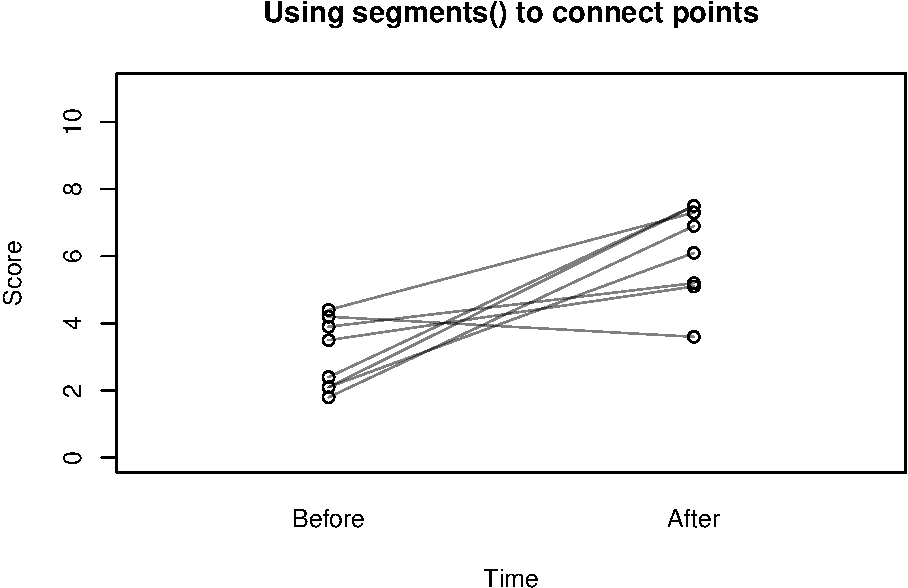
\includegraphics{YaRrr_files/figure-latex/segments-1} 

}

\caption{Connecting points with segments().}\label{fig:segments}
\end{figure}

The \texttt{grid()} function allows you to easily add grid lines to a
plot (you can customize your grid lines further with \texttt{lty},
\texttt{lwd}, and \texttt{col} arguments):

\begin{Shaded}
\begin{Highlighting}[]
\CommentTok{# Add gridlines to a plot with grid()}
\KeywordTok{plot}\NormalTok{(pirates$age,}
     \NormalTok{pirates$beard.length,}
     \DataTypeTok{pch =} \DecValTok{16}\NormalTok{,}
     \DataTypeTok{col =} \KeywordTok{gray}\NormalTok{(.}\DecValTok{1}\NormalTok{, .}\DecValTok{2}\NormalTok{), }\DataTypeTok{main =} \StringTok{"Add grid lines to a plot with grid()"}\NormalTok{)}

\CommentTok{# Add gridlines}
\KeywordTok{grid}\NormalTok{()}
\end{Highlighting}
\end{Shaded}

\begin{center}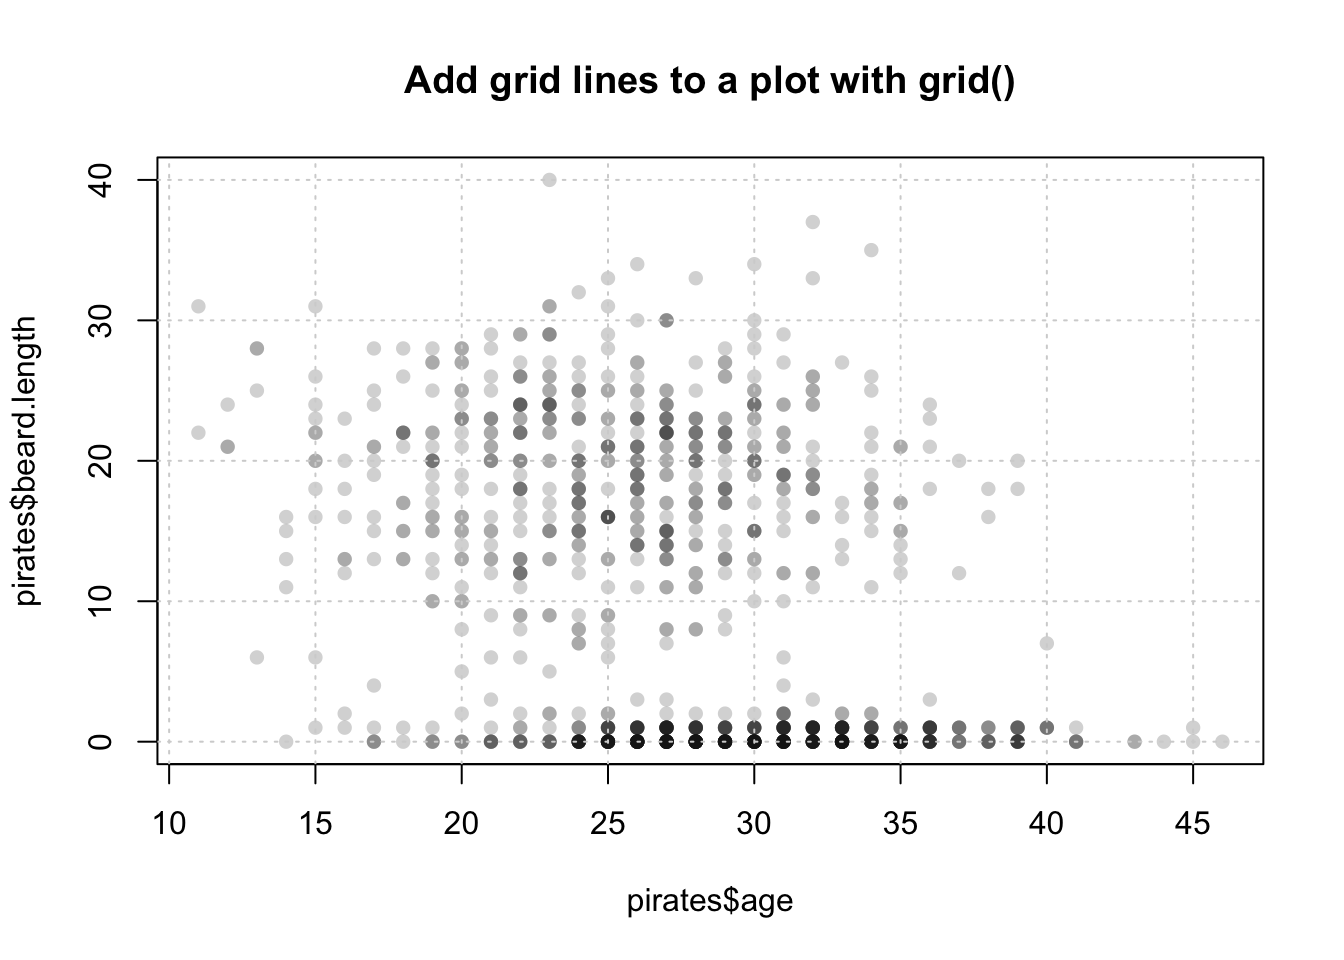
\includegraphics{YaRrr_files/figure-latex/unnamed-chunk-28-1} \end{center}

\subsection{\texorpdfstring{\texttt{text()}}{text()}}\label{text}

\begin{longtable}[]{@{}ll@{}}
\caption{\label{tab:textarguments} Arguments to
\texttt{text()}}\tabularnewline
\toprule
\begin{minipage}[b]{0.14\columnwidth}\raggedright\strut
Argument\strut
\end{minipage} & \begin{minipage}[b]{0.71\columnwidth}\raggedright\strut
Outcome\strut
\end{minipage}\tabularnewline
\midrule
\endfirsthead
\toprule
\begin{minipage}[b]{0.14\columnwidth}\raggedright\strut
Argument\strut
\end{minipage} & \begin{minipage}[b]{0.71\columnwidth}\raggedright\strut
Outcome\strut
\end{minipage}\tabularnewline
\midrule
\endhead
\begin{minipage}[t]{0.14\columnwidth}\raggedright\strut
\texttt{x}, \texttt{y}\strut
\end{minipage} & \begin{minipage}[t]{0.71\columnwidth}\raggedright\strut
Coordinates of the labels\strut
\end{minipage}\tabularnewline
\begin{minipage}[t]{0.14\columnwidth}\raggedright\strut
\texttt{labels}\strut
\end{minipage} & \begin{minipage}[t]{0.71\columnwidth}\raggedright\strut
Labels to be plotted\strut
\end{minipage}\tabularnewline
\begin{minipage}[t]{0.14\columnwidth}\raggedright\strut
\texttt{cex}\strut
\end{minipage} & \begin{minipage}[t]{0.71\columnwidth}\raggedright\strut
Size of the labels\strut
\end{minipage}\tabularnewline
\begin{minipage}[t]{0.14\columnwidth}\raggedright\strut
\texttt{adj}\strut
\end{minipage} & \begin{minipage}[t]{0.71\columnwidth}\raggedright\strut
Horizontal text adjustment. \texttt{adj\ =\ 0} is left justified,
\texttt{adj\ =\ .5} is centered, and \texttt{adj\ =\ 1} is
right-justified\strut
\end{minipage}\tabularnewline
\begin{minipage}[t]{0.14\columnwidth}\raggedright\strut
\texttt{pos}\strut
\end{minipage} & \begin{minipage}[t]{0.71\columnwidth}\raggedright\strut
Position of the labels relative to the coordinates. \texttt{pos\ =\ 1},
puts the label below the coordinates, while 2, 3, and 4 put it to the
left, top and right of the coordinates respectively\strut
\end{minipage}\tabularnewline
\bottomrule
\end{longtable}

With \texttt{text()}, you can add text to a plot. You can use
\texttt{text()} to highlight specific points of interest in the plot, or
to add information (like a third variable) for every point in a plot.
For example, the following code adds the three words ``Put'', ``Text'',
and ``Here'' at the coordinates (1, 9), (5, 5), and (9, 1) respectively.
See Figure \ref{fig:puttexthere} for the plot:

\begin{Shaded}
\begin{Highlighting}[]
\KeywordTok{plot}\NormalTok{(}\DecValTok{1}\NormalTok{, }
     \DataTypeTok{xlim =} \KeywordTok{c}\NormalTok{(}\DecValTok{0}\NormalTok{, }\DecValTok{10}\NormalTok{), }
     \DataTypeTok{ylim =} \KeywordTok{c}\NormalTok{(}\DecValTok{0}\NormalTok{, }\DecValTok{10}\NormalTok{), }
     \DataTypeTok{type =} \StringTok{"n"}\NormalTok{)}

\KeywordTok{text}\NormalTok{(}\DataTypeTok{x =} \KeywordTok{c}\NormalTok{(}\DecValTok{1}\NormalTok{, }\DecValTok{5}\NormalTok{, }\DecValTok{9}\NormalTok{),}
     \DataTypeTok{y =} \KeywordTok{c}\NormalTok{(}\DecValTok{9}\NormalTok{, }\DecValTok{5}\NormalTok{, }\DecValTok{1}\NormalTok{),}
     \DataTypeTok{labels =} \KeywordTok{c}\NormalTok{(}\StringTok{"Put"}\NormalTok{, }\StringTok{"text"}\NormalTok{, }\StringTok{"here"}\NormalTok{))}
\end{Highlighting}
\end{Shaded}

\begin{figure}

{\centering 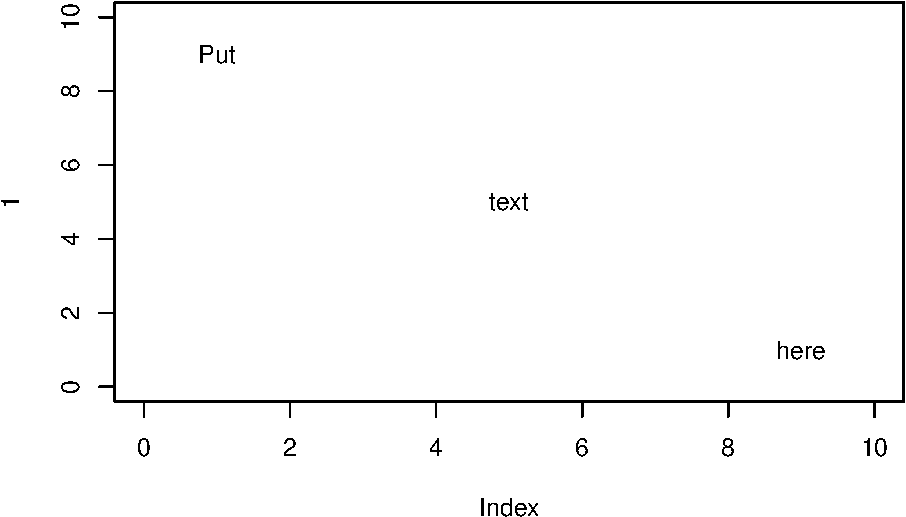
\includegraphics{YaRrr_files/figure-latex/puttexthere-1} 

}

\caption{Adding text to a plot with text()}\label{fig:puttexthere}
\end{figure}

You can do some cool things with \texttt{text()}, in Figure
\ref{fig:textlabels} I create a scatterplot of data, and add data labels
above each point by including the \texttt{pos\ =\ 3} argument:

\begin{Shaded}
\begin{Highlighting}[]
\CommentTok{# Create data vectors}
\NormalTok{height <-}\StringTok{ }\KeywordTok{c}\NormalTok{(}\DecValTok{156}\NormalTok{, }\DecValTok{175}\NormalTok{, }\DecValTok{160}\NormalTok{, }\DecValTok{172}\NormalTok{, }\DecValTok{159}\NormalTok{, }\DecValTok{165}\NormalTok{, }\DecValTok{178}\NormalTok{)}
\NormalTok{weight <-}\StringTok{ }\KeywordTok{c}\NormalTok{(}\DecValTok{65}\NormalTok{, }\DecValTok{74}\NormalTok{, }\DecValTok{69}\NormalTok{, }\DecValTok{72}\NormalTok{, }\DecValTok{66}\NormalTok{, }\DecValTok{75}\NormalTok{, }\DecValTok{75}\NormalTok{)}
\NormalTok{id <-}\StringTok{ }\KeywordTok{c}\NormalTok{(}\StringTok{"andrew"}\NormalTok{, }\StringTok{"heidi"}\NormalTok{, }\StringTok{"becki"}\NormalTok{, }\StringTok{"madisen"}\NormalTok{, }\StringTok{"david"}\NormalTok{, }\StringTok{"vincent"}\NormalTok{, }\StringTok{"jack"}\NormalTok{)}

\CommentTok{# Plot data}
\KeywordTok{plot}\NormalTok{(}\DataTypeTok{x =} \NormalTok{height, }
     \DataTypeTok{y =} \NormalTok{weight, }
     \DataTypeTok{xlim =} \KeywordTok{c}\NormalTok{(}\DecValTok{155}\NormalTok{, }\DecValTok{180}\NormalTok{), }
     \DataTypeTok{ylim =} \KeywordTok{c}\NormalTok{(}\DecValTok{65}\NormalTok{, }\DecValTok{80}\NormalTok{), }
     \DataTypeTok{pch =} \DecValTok{16}\NormalTok{,}
     \DataTypeTok{col =} \NormalTok{yarrr::}\KeywordTok{piratepal}\NormalTok{(}\StringTok{"xmen"}\NormalTok{))}

\CommentTok{# Add id labels}
\KeywordTok{text}\NormalTok{(}\DataTypeTok{x =} \NormalTok{height, }
     \DataTypeTok{y =} \NormalTok{weight,}
     \DataTypeTok{labels =} \NormalTok{id, }
     \DataTypeTok{pos =} \DecValTok{3}\NormalTok{)            }\CommentTok{# Put labels above the points}
\end{Highlighting}
\end{Shaded}

\begin{figure}

{\centering 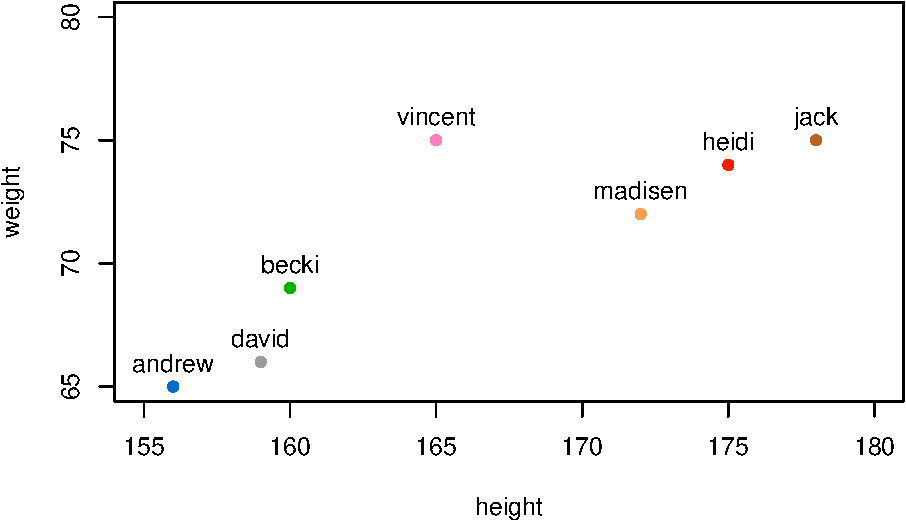
\includegraphics{YaRrr_files/figure-latex/textlabels-1} 

}

\caption{Adding labels to points with text()}\label{fig:textlabels}
\end{figure}

When entering text in the \texttt{labels} argument, keep in mind that R
will, by default, plot the entire text in one line. However, if you are
adding a long text string (like a sentence), you may want to separate
the text into separate lines. To do this, add the text
\texttt{\textbackslash{}n} where you want new lines to start. Look at
Figure \ref{fig:manylines} for an example.

\begin{Shaded}
\begin{Highlighting}[]
\KeywordTok{plot}\NormalTok{(}\DecValTok{1}\NormalTok{, }
     \DataTypeTok{type =} \StringTok{"n"}\NormalTok{,}
     \DataTypeTok{main =} \StringTok{"The }\CharTok{\textbackslash{}\textbackslash{}}\StringTok{n tag"}\NormalTok{,}
     \DataTypeTok{xlab =} \StringTok{""}\NormalTok{, }\DataTypeTok{ylab =} \StringTok{""}\NormalTok{)}

\CommentTok{# Text withoutbreaks}
\KeywordTok{text}\NormalTok{(}\DataTypeTok{x =} \DecValTok{1}\NormalTok{, }\DataTypeTok{y =} \FloatTok{1.3}\NormalTok{, }\DataTypeTok{labels =} \StringTok{"Text without }\CharTok{\textbackslash{}\textbackslash{}}\StringTok{n"}\NormalTok{, }\DataTypeTok{font =} \DecValTok{2}\NormalTok{)}
\KeywordTok{text}\NormalTok{(}\DataTypeTok{x =} \DecValTok{1}\NormalTok{, }\DataTypeTok{y =} \FloatTok{1.2}\NormalTok{,}
     \DataTypeTok{labels =} \StringTok{"Haikus are easy. But sometimes they don't make sense. Refrigerator"}\NormalTok{,}
     \DataTypeTok{font =} \DecValTok{3}\NormalTok{) }\CommentTok{# italic font}

\KeywordTok{abline}\NormalTok{(}\DataTypeTok{h =} \DecValTok{1}\NormalTok{, }\DataTypeTok{lty =} \DecValTok{2}\NormalTok{)}
\CommentTok{# Text with  breaks}
\KeywordTok{text}\NormalTok{(}\DataTypeTok{x =} \DecValTok{1}\NormalTok{, }\DataTypeTok{y =} \NormalTok{.}\DecValTok{92}\NormalTok{, }\DataTypeTok{labels =} \StringTok{"Text with }\CharTok{\textbackslash{}\textbackslash{}}\StringTok{n"}\NormalTok{, }\DataTypeTok{font =} \DecValTok{2}\NormalTok{)}
\KeywordTok{text}\NormalTok{(}\DataTypeTok{x =} \DecValTok{1}\NormalTok{, }\DataTypeTok{y =} \NormalTok{.}\DecValTok{7}\NormalTok{,}
     \DataTypeTok{labels =} \StringTok{"Haikus are easy}\CharTok{\textbackslash{}n}\StringTok{But sometimes they don't make sense}\CharTok{\textbackslash{}n}\StringTok{Refrigerator"}\NormalTok{,}
     \DataTypeTok{font =} \DecValTok{3}\NormalTok{)   }\CommentTok{# italic font}
\end{Highlighting}
\end{Shaded}

\begin{figure}

{\centering 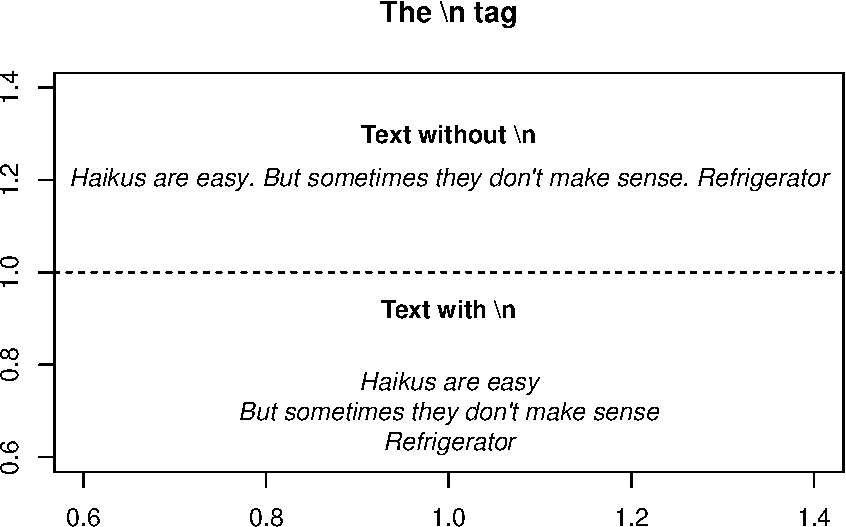
\includegraphics{YaRrr_files/figure-latex/manylines-1} 

}

\caption{Break up lines in text with 
.}\label{fig:manylines}
\end{figure}

\subsection{\texorpdfstring{Combining text and numbers with
\texttt{paste()}}{Combining text and numbers with paste()}}\label{combining-text-and-numbers-with-paste}

A common way to use text in a plot, either in the main title of a plot
or using the \texttt{text()}function, is to combine text with numerical
data. For example, you may want to include the text ``Mean = 3.14'' in a
plot to show that the mean of the data is 3.14. But how can we combine
numerical data with text? In R, we can do this with the \texttt{paste()}
function:

The paste function will be helpful to you anytime you want to combine
either multiple strings, or text and strings together. For example,
let's say you want to write text in a plot that says
\texttt{The\ mean\ of\ these\ data\ are\ XXX}, where XXX is replaced by
the group mean. To do this, just include the main text and the object
referring to the numerical mean as arguments to \texttt{paste()}. In
Figure X I plot the chicken weights over time, and add text to the plot
specifying the overall mean of weights.

\begin{Shaded}
\begin{Highlighting}[]
\CommentTok{# Create the plot}
\KeywordTok{plot}\NormalTok{(}\DataTypeTok{x =} \NormalTok{ChickWeight$Time,}
     \DataTypeTok{y =} \NormalTok{ChickWeight$weight, }
     \DataTypeTok{col =} \KeywordTok{gray}\NormalTok{(.}\DecValTok{3}\NormalTok{, .}\DecValTok{5}\NormalTok{), }
     \DataTypeTok{pch =} \DecValTok{16}\NormalTok{,}
     \DataTypeTok{main =} \StringTok{"Combining text with numeric scalers using paste()"}\NormalTok{)}

\CommentTok{# Add reference line}
\KeywordTok{abline}\NormalTok{(}\DataTypeTok{h =} \KeywordTok{mean}\NormalTok{(ChickWeight$weight), }
       \DataTypeTok{lty =} \DecValTok{2}\NormalTok{)}

\CommentTok{# Add text}
\KeywordTok{text}\NormalTok{(}\DataTypeTok{x =} \DecValTok{3}\NormalTok{, }
     \DataTypeTok{y =} \KeywordTok{mean}\NormalTok{(ChickWeight$weight), }
     \DataTypeTok{labels =} \KeywordTok{paste}\NormalTok{(}\StringTok{"Mean weight ="}\NormalTok{, }
                    \KeywordTok{round}\NormalTok{(}\KeywordTok{mean}\NormalTok{(ChickWeight$weight), }\DecValTok{2}\NormalTok{)),}
     \DataTypeTok{pos =} \DecValTok{3}\NormalTok{)}
\end{Highlighting}
\end{Shaded}

\begin{center}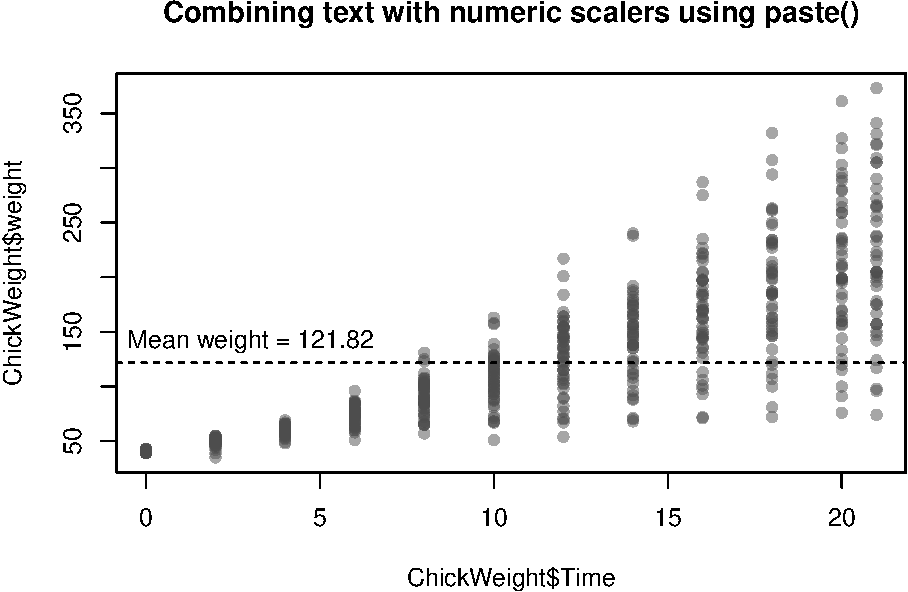
\includegraphics{YaRrr_files/figure-latex/unnamed-chunk-29-1} \end{center}

\subsection{\texorpdfstring{\texttt{curve()}}{curve()}}\label{curve}

\begin{longtable}[]{@{}ll@{}}
\caption{\label{tab:curvearguments} Arguments to
\texttt{curve()}}\tabularnewline
\toprule
\begin{minipage}[b]{0.14\columnwidth}\raggedright\strut
Argument\strut
\end{minipage} & \begin{minipage}[b]{0.71\columnwidth}\raggedright\strut
Outcome\strut
\end{minipage}\tabularnewline
\midrule
\endfirsthead
\toprule
\begin{minipage}[b]{0.14\columnwidth}\raggedright\strut
Argument\strut
\end{minipage} & \begin{minipage}[b]{0.71\columnwidth}\raggedright\strut
Outcome\strut
\end{minipage}\tabularnewline
\midrule
\endhead
\begin{minipage}[t]{0.14\columnwidth}\raggedright\strut
\texttt{expr}\strut
\end{minipage} & \begin{minipage}[t]{0.71\columnwidth}\raggedright\strut
The name of a function written as a function of \texttt{x} that returns
a single vector. You can either use base functions in R like
\texttt{expr\ =\ \$x\^{}2\$}, \texttt{expr\ =\ x\ +\ 4\ -\ 2}, or use
your own custom functions such as \texttt{expr\ =\ my.fun}, where
\texttt{my.fun} is previously defined (e.g.;
\texttt{my.fun\ \textless{}-\ function(x)\ \{dnorm(x,\ mean\ =\ 10,\ sd\ =\ 3)})\strut
\end{minipage}\tabularnewline
\begin{minipage}[t]{0.14\columnwidth}\raggedright\strut
\texttt{from,\ to}\strut
\end{minipage} & \begin{minipage}[t]{0.71\columnwidth}\raggedright\strut
The starting (\texttt{from}) and ending (\texttt{to}) value of x to be
plotted.\strut
\end{minipage}\tabularnewline
\begin{minipage}[t]{0.14\columnwidth}\raggedright\strut
\texttt{add}\strut
\end{minipage} & \begin{minipage}[t]{0.71\columnwidth}\raggedright\strut
A logical value indicating whether or not to add the curve to an
existing plot. If \texttt{add\ =\ FALSE}, then \texttt{curve()} will act
like a high-level plotting function and create a new plot. If
\texttt{add\ =\ TRUE}, then \texttt{curve()} will act like a low-level
plotting function.\strut
\end{minipage}\tabularnewline
\begin{minipage}[t]{0.14\columnwidth}\raggedright\strut
\strut
\end{minipage}\tabularnewline
\begin{minipage}[t]{0.14\columnwidth}\raggedright\strut
\texttt{lty,\ lwd,\ col}\strut
\end{minipage} & \begin{minipage}[t]{0.71\columnwidth}\raggedright\strut
Additional standard line arguments\strut
\end{minipage}\tabularnewline
\bottomrule
\end{longtable}

The \texttt{curve()} function allows you to add a line showing a
specific function or equation to a plot. For example, to add the
function \(x^2\) to a plot from the x-values -10 to 10, you can run the
code:

\begin{Shaded}
\begin{Highlighting}[]
\CommentTok{# Plot the function x^2 from -10 to +10}
\KeywordTok{curve}\NormalTok{(}\DataTypeTok{expr =} \NormalTok{x^}\DecValTok{2}\NormalTok{, }
      \DataTypeTok{from =} \NormalTok{-}\DecValTok{10}\NormalTok{, }
      \DataTypeTok{to =} \DecValTok{10}\NormalTok{, }\DataTypeTok{lwd =} \DecValTok{2}\NormalTok{)}
\end{Highlighting}
\end{Shaded}

\begin{center}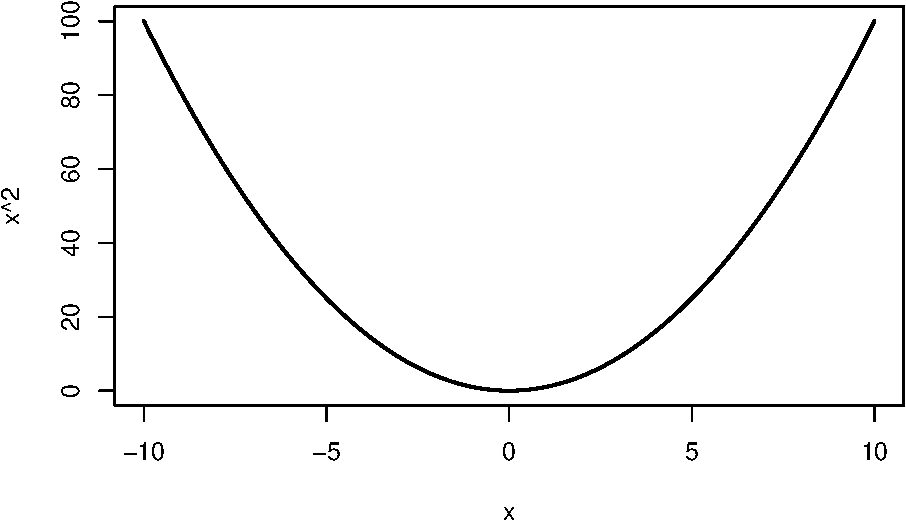
\includegraphics{YaRrr_files/figure-latex/unnamed-chunk-30-1} \end{center}

If you want to add a custom function to a plot, you can define the
function and then use that function name as the argument to
\texttt{expr}. For example, to plot the normal distribution with a mean
of 10 and standard deviation of 3, you can use this code:

\begin{Shaded}
\begin{Highlighting}[]
\CommentTok{# Plot the normal distribution with mean = 22 and sd = 3}

\CommentTok{# Create a function}
\NormalTok{my.fun <-}\StringTok{ }\NormalTok{function(x) \{}\KeywordTok{dnorm}\NormalTok{(x, }\DataTypeTok{mean =} \DecValTok{2}\NormalTok{, }\DataTypeTok{sd =} \DecValTok{3}\NormalTok{)\}}

\KeywordTok{curve}\NormalTok{(}\DataTypeTok{expr =} \NormalTok{my.fun, }
      \DataTypeTok{from =} \NormalTok{-}\DecValTok{10}\NormalTok{, }
      \DataTypeTok{to =} \DecValTok{10}\NormalTok{, }\DataTypeTok{lwd =} \DecValTok{2}\NormalTok{)}
\end{Highlighting}
\end{Shaded}

\begin{center}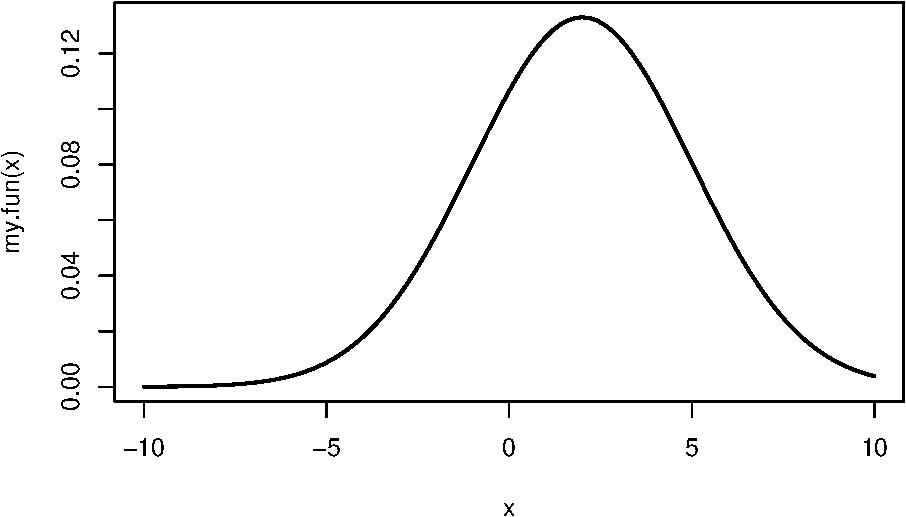
\includegraphics{YaRrr_files/figure-latex/unnamed-chunk-31-1} \end{center}

In Figure\textasciitilde{}\ref{fig:functionlines}, I use the
\texttt{curve()} function to create curves of several mathematical
formulas.

\begin{Shaded}
\begin{Highlighting}[]
\CommentTok{# Create plotting space}
\KeywordTok{plot}\NormalTok{(}\DecValTok{1}\NormalTok{, }
     \DataTypeTok{xlim =} \KeywordTok{c}\NormalTok{(-}\DecValTok{5}\NormalTok{, }\DecValTok{5}\NormalTok{), }\DataTypeTok{ylim =} \KeywordTok{c}\NormalTok{(-}\DecValTok{5}\NormalTok{, }\DecValTok{5}\NormalTok{),}
     \DataTypeTok{type =} \StringTok{"n"}\NormalTok{, }
     \DataTypeTok{main =} \StringTok{"Plotting function lines with curve()"}\NormalTok{,}
     \DataTypeTok{ylab =} \StringTok{""}\NormalTok{, }\DataTypeTok{xlab =} \StringTok{""}\NormalTok{)}

\CommentTok{# Add x and y-axis lines}
\KeywordTok{abline}\NormalTok{(}\DataTypeTok{h =} \DecValTok{0}\NormalTok{)}
\KeywordTok{abline}\NormalTok{(}\DataTypeTok{v =} \DecValTok{0}\NormalTok{)}

\CommentTok{# set up colors}
\NormalTok{col.vec <-}\StringTok{ }\KeywordTok{piratepal}\NormalTok{(}\StringTok{"google"}\NormalTok{)}

\CommentTok{# x ^ 2}
\KeywordTok{curve}\NormalTok{(}\DataTypeTok{expr =} \NormalTok{x^}\DecValTok{2}\NormalTok{, }\DataTypeTok{from =} \NormalTok{-}\DecValTok{5}\NormalTok{, }\DataTypeTok{to =} \DecValTok{5}\NormalTok{,}
      \DataTypeTok{add =} \OtherTok{TRUE}\NormalTok{, }\DataTypeTok{lwd =} \DecValTok{3}\NormalTok{, }\DataTypeTok{col =} \NormalTok{col.vec[}\DecValTok{1}\NormalTok{])}

\CommentTok{# sin(x)}
\KeywordTok{curve}\NormalTok{(}\DataTypeTok{expr =} \NormalTok{sin, }\DataTypeTok{from =} \NormalTok{-}\DecValTok{5}\NormalTok{, }\DataTypeTok{to =} \DecValTok{5}\NormalTok{,}
      \DataTypeTok{add =} \OtherTok{TRUE}\NormalTok{, }\DataTypeTok{lwd =} \DecValTok{3}\NormalTok{, }\DataTypeTok{col =} \NormalTok{col.vec[}\DecValTok{2}\NormalTok{])}

\CommentTok{# dnorm(mean = 2, sd = .2)}
\NormalTok{my.fun <-}\StringTok{ }\NormalTok{function(x) \{}\KeywordTok{return}\NormalTok{(}\KeywordTok{dnorm}\NormalTok{(x, }\DataTypeTok{mean =} \DecValTok{2}\NormalTok{, }\DataTypeTok{sd =} \NormalTok{.}\DecValTok{2}\NormalTok{))\}}
\KeywordTok{curve}\NormalTok{(}\DataTypeTok{expr =} \NormalTok{my.fun, }
      \DataTypeTok{from =} \NormalTok{-}\DecValTok{5}\NormalTok{, }\DataTypeTok{to =} \DecValTok{5}\NormalTok{,}
      \DataTypeTok{add =} \OtherTok{TRUE}\NormalTok{, }
      \DataTypeTok{lwd =} \DecValTok{3}\NormalTok{, }\DataTypeTok{col =} \NormalTok{col.vec[}\DecValTok{3}\NormalTok{])}

\CommentTok{# Add legend}
\KeywordTok{legend}\NormalTok{(}\StringTok{"bottomright"}\NormalTok{,}
       \DataTypeTok{legend =} \KeywordTok{c}\NormalTok{(}\StringTok{"x^2"}\NormalTok{, }\StringTok{"sin(x)"}\NormalTok{, }\StringTok{"dnorm(x, 2, .2)"}\NormalTok{),}
       \DataTypeTok{col =} \NormalTok{col.vec[}\DecValTok{1}\NormalTok{:}\DecValTok{3}\NormalTok{], }
       \DataTypeTok{lwd =} \DecValTok{3}\NormalTok{)}
\end{Highlighting}
\end{Shaded}

\begin{figure}

{\centering 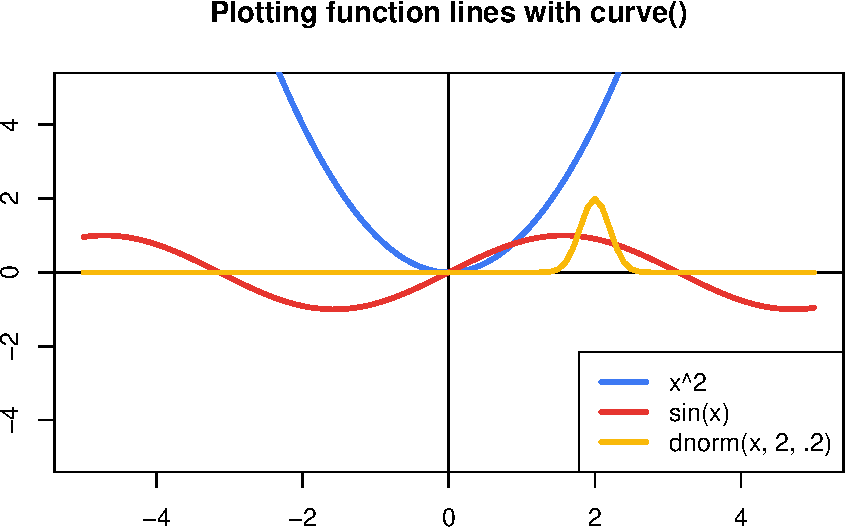
\includegraphics{YaRrr_files/figure-latex/functionlines-1} 

}

\caption{Drawing function lines with curve()}\label{fig:functionlines}
\end{figure}

\subsection{\texorpdfstring{\texttt{legend()}}{legend()}}\label{legend}

\begin{longtable}[]{@{}ll@{}}
\caption{\label{tab:legendarguments} Arguments to
\texttt{legend()}}\tabularnewline
\toprule
\begin{minipage}[b]{0.14\columnwidth}\raggedright\strut
Argument\strut
\end{minipage} & \begin{minipage}[b]{0.71\columnwidth}\raggedright\strut
Outcome\strut
\end{minipage}\tabularnewline
\midrule
\endfirsthead
\toprule
\begin{minipage}[b]{0.14\columnwidth}\raggedright\strut
Argument\strut
\end{minipage} & \begin{minipage}[b]{0.71\columnwidth}\raggedright\strut
Outcome\strut
\end{minipage}\tabularnewline
\midrule
\endhead
\begin{minipage}[t]{0.14\columnwidth}\raggedright\strut
\texttt{x,\ y}\strut
\end{minipage} & \begin{minipage}[t]{0.71\columnwidth}\raggedright\strut
Coordinates of the legend - for example, \texttt{x\ =\ 0,\ y\ =\ 0} will
put the text at the coordinates (0, 0). Alternatively, you can enter a
string indicating where to put the legend (i.e.; \texttt{"topright"},
\texttt{"topleft"}). For example, \texttt{"bottomright"} will always put
the legend at the bottom right corner of the plot.\strut
\end{minipage}\tabularnewline
\begin{minipage}[t]{0.14\columnwidth}\raggedright\strut
\texttt{labels}\strut
\end{minipage} & \begin{minipage}[t]{0.71\columnwidth}\raggedright\strut
A string vector specifying the text in the legend. For example,
\texttt{legend\ =\ c("Males,\ "Females")} will create two groups with
names Males and Females.\strut
\end{minipage}\tabularnewline
\begin{minipage}[t]{0.14\columnwidth}\raggedright\strut
\texttt{pch,\ lty,\ lwd,\ col,\ pt.bg,\ ...}\strut
\end{minipage} & \begin{minipage}[t]{0.71\columnwidth}\raggedright\strut
Additional arguments specifying symbol types (\texttt{pch}), line types
(\texttt{lty}), line widths (\texttt{lwd}), background color of symbol
types 21 through 25 (\texttt{pt.bg}) and several other optional
arguments. See \texttt{?legend} for a complete list\strut
\end{minipage}\tabularnewline
\bottomrule
\end{longtable}

The last low-level plotting function that we'll go over in detail is
\texttt{legend()} which adds a legend to a plot. For example, to add a
legend to to bottom-right of an existing graph where data from females
are plotted in blue circles and data from males are plotted in pink
circles, you'd use the following code:

\begin{Shaded}
\begin{Highlighting}[]
\CommentTok{# Add a legend to the bottom right of a plot}

\KeywordTok{legend}\NormalTok{(}\StringTok{"bottomright"}\NormalTok{,                  }\CommentTok{# Put legend in bottom right of graph}
       \DataTypeTok{legend =} \KeywordTok{c}\NormalTok{(}\StringTok{"Females"}\NormalTok{, }\StringTok{"Males"}\NormalTok{), }\CommentTok{# Names of groups}
       \DataTypeTok{col =} \KeywordTok{c}\NormalTok{(}\StringTok{"blue"}\NormalTok{, }\StringTok{"orange"}\NormalTok{),      }\CommentTok{# Colors of symbols}
       \DataTypeTok{pch =} \KeywordTok{c}\NormalTok{(}\DecValTok{16}\NormalTok{, }\DecValTok{16}\NormalTok{))                }\CommentTok{# Symbol types}
\end{Highlighting}
\end{Shaded}

In Figure \ref{fig:legendexample} I use this code to add a legend to
plot containing data from males and females:

\begin{Shaded}
\begin{Highlighting}[]
\CommentTok{# Create plot with data from females}
\KeywordTok{plot}\NormalTok{(}\DataTypeTok{x =} \NormalTok{pirates$age[pirates$sex ==}\StringTok{ "female"}\NormalTok{], }
     \DataTypeTok{y =} \NormalTok{pirates$tattoos[pirates$sex ==}\StringTok{ "female"}\NormalTok{],}
     \DataTypeTok{xlim =} \KeywordTok{c}\NormalTok{(}\DecValTok{0}\NormalTok{, }\DecValTok{50}\NormalTok{),}
     \DataTypeTok{ylim =} \KeywordTok{c}\NormalTok{(}\DecValTok{0}\NormalTok{, }\DecValTok{20}\NormalTok{),}
     \DataTypeTok{pch =} \DecValTok{16}\NormalTok{, }\DataTypeTok{col =} \NormalTok{yarrr::}\KeywordTok{transparent}\NormalTok{(}\StringTok{"red"}\NormalTok{, .}\DecValTok{7}\NormalTok{),}
     \DataTypeTok{xlab =} \StringTok{"Age"}\NormalTok{, }\DataTypeTok{ylab =} \StringTok{"Tattoos"}\NormalTok{, }
     \DataTypeTok{main =} \StringTok{"Adding a legend with legend()"}\NormalTok{)}

\CommentTok{# Add data from males}
\KeywordTok{points}\NormalTok{(}\DataTypeTok{x =} \NormalTok{pirates$age[pirates$sex ==}\StringTok{ "male"}\NormalTok{], }
       \DataTypeTok{y =} \NormalTok{pirates$tattoos[pirates$sex ==}\StringTok{ "male"}\NormalTok{],}
       \DataTypeTok{pch =} \DecValTok{16}\NormalTok{, }\DataTypeTok{col =} \NormalTok{yarrr::}\KeywordTok{transparent}\NormalTok{(}\StringTok{"blue"}\NormalTok{, .}\DecValTok{7}\NormalTok{))}

\CommentTok{# Add legend}
\KeywordTok{legend}\NormalTok{(}\StringTok{"bottomright"}\NormalTok{,}
       \DataTypeTok{legend =} \KeywordTok{c}\NormalTok{(}\StringTok{"Females"}\NormalTok{, }\StringTok{"Males"}\NormalTok{),}
       \DataTypeTok{col =} \KeywordTok{transparent}\NormalTok{(}\KeywordTok{c}\NormalTok{(}\StringTok{'red'}\NormalTok{, }\StringTok{'blue'}\NormalTok{), .}\DecValTok{5}\NormalTok{),}
       \DataTypeTok{pch =} \KeywordTok{c}\NormalTok{(}\DecValTok{16}\NormalTok{, }\DecValTok{16}\NormalTok{),}
       \DataTypeTok{bg =} \StringTok{"white"}\NormalTok{)}
\end{Highlighting}
\end{Shaded}

\begin{figure}

{\centering 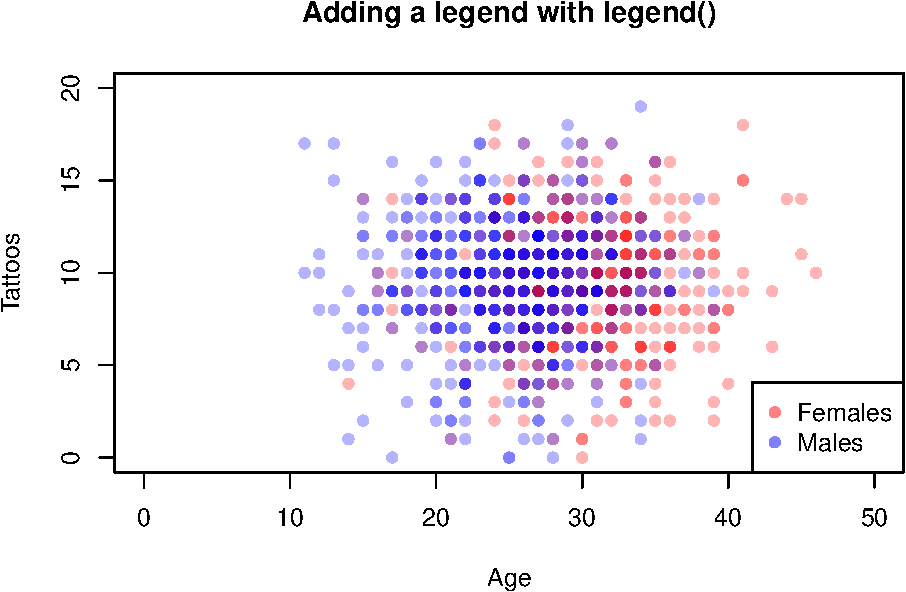
\includegraphics{YaRrr_files/figure-latex/legendexample-1} 

}

\caption{Adding a legend to a plot with legend().}\label{fig:legendexample}
\end{figure}

There are many more low-level plotting functions that can add additional
elements to your plots. Here are some I use. To see examples of how to
use each one, check out their associated help menus.

\begin{Shaded}
\begin{Highlighting}[]
\KeywordTok{plot}\NormalTok{(}\DecValTok{1}\NormalTok{, }\DataTypeTok{xlim =} \KeywordTok{c}\NormalTok{(}\DecValTok{1}\NormalTok{, }\DecValTok{100}\NormalTok{), }\DataTypeTok{ylim =} \KeywordTok{c}\NormalTok{(}\DecValTok{1}\NormalTok{, }\DecValTok{100}\NormalTok{),}
     \DataTypeTok{type =} \StringTok{"n"}\NormalTok{, }\DataTypeTok{xaxt =} \StringTok{"n"}\NormalTok{, }\DataTypeTok{yaxt =} \StringTok{"n"}\NormalTok{,}
     \DataTypeTok{ylab =} \StringTok{""}\NormalTok{, }\DataTypeTok{xlab =} \StringTok{""}\NormalTok{, }\DataTypeTok{main =} \StringTok{"Adding simple figures to a plot"}\NormalTok{)}

\KeywordTok{text}\NormalTok{(}\DecValTok{25}\NormalTok{, }\DecValTok{95}\NormalTok{, }\DataTypeTok{labels =} \StringTok{"rect()"}\NormalTok{)}
\KeywordTok{rect}\NormalTok{(}\DataTypeTok{xleft =} \DecValTok{10}\NormalTok{, }\DataTypeTok{ybottom =} \DecValTok{70}\NormalTok{,}
     \DataTypeTok{xright =} \DecValTok{40}\NormalTok{, }\DataTypeTok{ytop =} \DecValTok{90}\NormalTok{, }\DataTypeTok{lwd =} \DecValTok{2}\NormalTok{, }\DataTypeTok{col =} \StringTok{"coral"}\NormalTok{)}

\KeywordTok{text}\NormalTok{(}\DecValTok{25}\NormalTok{, }\DecValTok{60}\NormalTok{, }\DataTypeTok{labels =} \StringTok{"polygon()"}\NormalTok{)}
\KeywordTok{polygon}\NormalTok{(}\DataTypeTok{x =} \KeywordTok{runif}\NormalTok{(}\DecValTok{6}\NormalTok{, }\DecValTok{15}\NormalTok{, }\DecValTok{35}\NormalTok{),}
        \DataTypeTok{y =} \KeywordTok{runif}\NormalTok{(}\DecValTok{6}\NormalTok{, }\DecValTok{40}\NormalTok{, }\DecValTok{55}\NormalTok{),}
        \DataTypeTok{col =} \StringTok{"skyblue"}\NormalTok{)}

\KeywordTok{text}\NormalTok{(}\DecValTok{25}\NormalTok{, }\DecValTok{30}\NormalTok{, }\DataTypeTok{labels =} \StringTok{"segments()"}\NormalTok{)}
\KeywordTok{segments}\NormalTok{(}\DataTypeTok{x0 =} \KeywordTok{runif}\NormalTok{(}\DecValTok{5}\NormalTok{, }\DecValTok{10}\NormalTok{, }\DecValTok{40}\NormalTok{),}
         \DataTypeTok{y0 =} \KeywordTok{runif}\NormalTok{(}\DecValTok{5}\NormalTok{, }\DecValTok{5}\NormalTok{, }\DecValTok{25}\NormalTok{),}
         \DataTypeTok{x1 =} \KeywordTok{runif}\NormalTok{(}\DecValTok{5}\NormalTok{, }\DecValTok{10}\NormalTok{, }\DecValTok{40}\NormalTok{),}
         \DataTypeTok{y1 =} \KeywordTok{runif}\NormalTok{(}\DecValTok{5}\NormalTok{, }\DecValTok{5}\NormalTok{, }\DecValTok{25}\NormalTok{), }
         \DataTypeTok{lwd =} \DecValTok{2}\NormalTok{)}

\KeywordTok{text}\NormalTok{(}\DecValTok{75}\NormalTok{, }\DecValTok{95}\NormalTok{, }\DataTypeTok{labels =} \StringTok{"symbols(circles)"}\NormalTok{)}
\KeywordTok{symbols}\NormalTok{(}\DataTypeTok{x =} \KeywordTok{runif}\NormalTok{(}\DecValTok{3}\NormalTok{, }\DecValTok{60}\NormalTok{, }\DecValTok{90}\NormalTok{),}
        \DataTypeTok{y =} \KeywordTok{runif}\NormalTok{(}\DecValTok{3}\NormalTok{, }\DecValTok{60}\NormalTok{, }\DecValTok{70}\NormalTok{),}
        \DataTypeTok{circles =} \KeywordTok{c}\NormalTok{(}\DecValTok{1}\NormalTok{, .}\DecValTok{1}\NormalTok{, .}\DecValTok{3}\NormalTok{),}
        \DataTypeTok{add =} \OtherTok{TRUE}\NormalTok{, }\DataTypeTok{bg =} \KeywordTok{gray}\NormalTok{(.}\DecValTok{5}\NormalTok{, .}\DecValTok{1}\NormalTok{))}

\KeywordTok{text}\NormalTok{(}\DecValTok{75}\NormalTok{, }\DecValTok{30}\NormalTok{, }\DataTypeTok{labels =} \StringTok{"arrows()"}\NormalTok{)}
\KeywordTok{arrows}\NormalTok{(}\DataTypeTok{x0 =} \KeywordTok{runif}\NormalTok{(}\DecValTok{3}\NormalTok{, }\DecValTok{60}\NormalTok{, }\DecValTok{90}\NormalTok{),}
       \DataTypeTok{y0 =} \KeywordTok{runif}\NormalTok{(}\DecValTok{3}\NormalTok{, }\DecValTok{10}\NormalTok{, }\DecValTok{25}\NormalTok{),}
       \DataTypeTok{x1 =} \KeywordTok{runif}\NormalTok{(}\DecValTok{3}\NormalTok{, }\DecValTok{60}\NormalTok{, }\DecValTok{90}\NormalTok{),}
       \DataTypeTok{y1 =} \KeywordTok{runif}\NormalTok{(}\DecValTok{3}\NormalTok{, }\DecValTok{10}\NormalTok{, }\DecValTok{25}\NormalTok{),}
       \DataTypeTok{length =} \NormalTok{.}\DecValTok{1}\NormalTok{, }\DataTypeTok{lwd =} \DecValTok{2}\NormalTok{)}
\end{Highlighting}
\end{Shaded}

\begin{figure}

{\centering 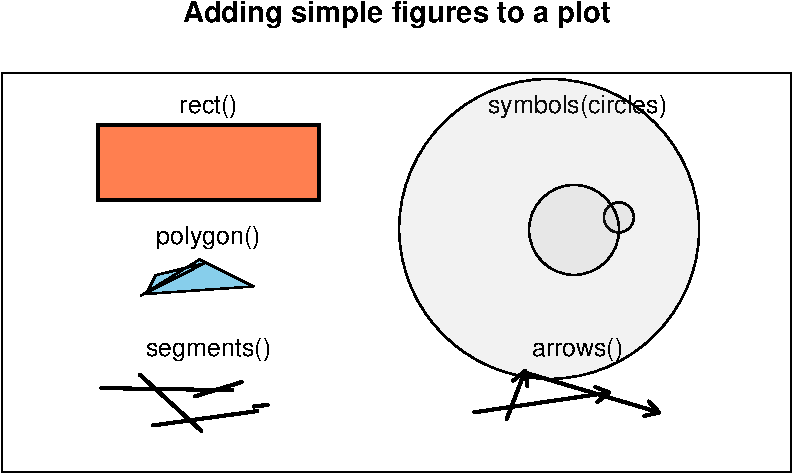
\includegraphics{YaRrr_files/figure-latex/simplefigures-1} 

}

\caption{Additional figures one can add to a plot with rect(), polygon(), segments(), symbols(), and arrows().}\label{fig:simplefigures}
\end{figure}

\section{\texorpdfstring{Saving plots to a file with \texttt{pdf()},
\texttt{jpeg()} and
\texttt{png()}}{Saving plots to a file with pdf(), jpeg() and png()}}\label{saving-plots-to-a-file-with-pdf-jpeg-and-png}

Once you've created a plot in R, you may wish to save it to a file so
you can use it in another document. To do this, you'll use either the
\texttt{pdf()}, \texttt{png()} or \texttt{jpeg()} functions. These
functions will save your plot to either a .pdf, .jpg, or .png file.

\begin{longtable}[]{@{}ll@{}}
\caption{\label{tab:pdfarguments} Arguments to \texttt{pdf()},
\texttt{jpeg()} and \texttt{png()}}\tabularnewline
\toprule
\begin{minipage}[b]{0.14\columnwidth}\raggedright\strut
Argument\strut
\end{minipage} & \begin{minipage}[b]{0.71\columnwidth}\raggedright\strut
Outcome\strut
\end{minipage}\tabularnewline
\midrule
\endfirsthead
\toprule
\begin{minipage}[b]{0.14\columnwidth}\raggedright\strut
Argument\strut
\end{minipage} & \begin{minipage}[b]{0.71\columnwidth}\raggedright\strut
Outcome\strut
\end{minipage}\tabularnewline
\midrule
\endhead
\begin{minipage}[t]{0.14\columnwidth}\raggedright\strut
\texttt{file}\strut
\end{minipage} & \begin{minipage}[t]{0.71\columnwidth}\raggedright\strut
The directory and name of the final plot entered as a string. For
example, to put a plot on my desktop, I'd write
\texttt{file\ =\ "/Users/nphillips/Desktop/plot.pdf"} when creating a
pdf, and \texttt{file\ =\ "/Users/nphillips/Desktop/plot.jpg"} when
creating a jpeg.\strut
\end{minipage}\tabularnewline
\begin{minipage}[t]{0.14\columnwidth}\raggedright\strut
\texttt{width,\ height}\strut
\end{minipage} & \begin{minipage}[t]{0.71\columnwidth}\raggedright\strut
The width and height of the final plot in inches.\strut
\end{minipage}\tabularnewline
\begin{minipage}[t]{0.14\columnwidth}\raggedright\strut
\texttt{dev.off()}\strut
\end{minipage} & \begin{minipage}[t]{0.71\columnwidth}\raggedright\strut
This is \emph{not} an argument to \texttt{pdf()} and \texttt{jpeg()}.
You just need to execute this code after creating the plot to finish
creating the image file (see examples).\strut
\end{minipage}\tabularnewline
\bottomrule
\end{longtable}

To use these functions to save files, you need to follow 3 steps:

\begin{enumerate}
\def\labelenumi{\arabic{enumi}.}
\tightlist
\item
  Execute the \texttt{pdf()} or \texttt{jpeg()} functions with
  \texttt{file,\ width,\ height} arguments.
\item
  Execute all your plotting code (e.g.;
  \texttt{plot(x\ =\ 1:10,\ y\ =\ 1:10)})
\item
  Complete the file by executing the command \texttt{dev.off()}. This
  tells R that you're done creating the file.
\end{enumerate}

The chunk below shows an example of the three steps in creating a pdf:

\begin{Shaded}
\begin{Highlighting}[]
\CommentTok{# Step 1: Call the pdf command to start the plot}
\KeywordTok{pdf}\NormalTok{(}\DataTypeTok{file =} \StringTok{"/Users/ndphillips/Desktop/My Plot.pdf"}\NormalTok{,   }\CommentTok{# The directory you want to save the file in}
    \DataTypeTok{width =} \DecValTok{4}\NormalTok{, }\CommentTok{# The width of the plot in inches}
    \DataTypeTok{height =} \DecValTok{4}\NormalTok{) }\CommentTok{# The height of the plot in inches}

\CommentTok{# Step 2: Create the plot with R code}
\KeywordTok{plot}\NormalTok{(}\DataTypeTok{x =} \DecValTok{1}\NormalTok{:}\DecValTok{10}\NormalTok{, }
     \DataTypeTok{y =} \DecValTok{1}\NormalTok{:}\DecValTok{10}\NormalTok{)}
\KeywordTok{abline}\NormalTok{(}\DataTypeTok{v =} \DecValTok{0}\NormalTok{) }\CommentTok{# Additional low-level plotting commands}
\KeywordTok{text}\NormalTok{(}\DataTypeTok{x =} \DecValTok{0}\NormalTok{, }\DataTypeTok{y =} \DecValTok{1}\NormalTok{, }\DataTypeTok{labels =} \StringTok{"Random text"}\NormalTok{)}

\CommentTok{# Step 3: Run dev.off() to create the file!}
\KeywordTok{dev.off}\NormalTok{()}
\end{Highlighting}
\end{Shaded}

You'll notice that after you close the plot with \texttt{dev.off()},
you'll see a message in the prompt like ``null device''. That's just R
telling you that you can now create plots in the main R plotting window
again.

The functions \texttt{pdf()}, \texttt{jpeg()}, and \texttt{png()} all
work the same way, they just return different file types. If you can,
use \texttt{pdf()} it saves the plot in a high quality format.

\section{Examples}\label{examples}

Figure \ref{fig:balloonplot} shows a modified version of a scatterplot I
call a \texttt{balloonplot}:

\begin{Shaded}
\begin{Highlighting}[]
\CommentTok{# Turn a boring scatterplot into a  balloonplot! }

\CommentTok{# Create some random correlated data}
\NormalTok{x <-}\StringTok{ }\KeywordTok{rnorm}\NormalTok{(}\DecValTok{50}\NormalTok{, }\DataTypeTok{mean =} \DecValTok{50}\NormalTok{, }\DataTypeTok{sd =} \DecValTok{10}\NormalTok{)}
\NormalTok{y <-}\StringTok{ }\NormalTok{x +}\StringTok{ }\KeywordTok{rnorm}\NormalTok{(}\DecValTok{50}\NormalTok{, }\DataTypeTok{mean =} \DecValTok{20}\NormalTok{, }\DataTypeTok{sd =} \DecValTok{8}\NormalTok{)}

\CommentTok{# Set up the plotting space}
\KeywordTok{plot}\NormalTok{(}\DecValTok{1}\NormalTok{, }
     \DataTypeTok{bty =} \StringTok{"n"}\NormalTok{,}
     \DataTypeTok{xlim =} \KeywordTok{c}\NormalTok{(}\DecValTok{0}\NormalTok{, }\DecValTok{100}\NormalTok{),}
     \DataTypeTok{ylim =} \KeywordTok{c}\NormalTok{(}\DecValTok{0}\NormalTok{, }\DecValTok{100}\NormalTok{),}
     \DataTypeTok{type =} \StringTok{"n"}\NormalTok{, }\DataTypeTok{xlab =} \StringTok{""}\NormalTok{, }\DataTypeTok{ylab =} \StringTok{""}\NormalTok{, }
     \DataTypeTok{main =} \StringTok{"Turning a scatterplot into a balloon plot!"}\NormalTok{)}

\CommentTok{# Add gridlines}
\KeywordTok{grid}\NormalTok{()}

\CommentTok{# Add Strings with segments()}
\KeywordTok{segments}\NormalTok{(}\DataTypeTok{x0 =} \NormalTok{x +}\StringTok{ }\KeywordTok{rnorm}\NormalTok{(}\KeywordTok{length}\NormalTok{(x), }\DataTypeTok{mean =} \DecValTok{0}\NormalTok{, }\DataTypeTok{sd =} \NormalTok{.}\DecValTok{5}\NormalTok{), }
         \DataTypeTok{y0 =} \NormalTok{y -}\StringTok{ }\DecValTok{10}\NormalTok{, }
         \DataTypeTok{x1 =} \NormalTok{x, }
         \DataTypeTok{y1 =} \NormalTok{y, }
         \DataTypeTok{col =} \KeywordTok{gray}\NormalTok{(.}\DecValTok{1}\NormalTok{, .}\DecValTok{95}\NormalTok{),}
         \DataTypeTok{lwd =} \NormalTok{.}\DecValTok{5}\NormalTok{)}

\CommentTok{# Add balloons}
\KeywordTok{points}\NormalTok{(x, y, }
       \DataTypeTok{cex =} \DecValTok{2}\NormalTok{, }\CommentTok{# Size of the balloons}
       \DataTypeTok{pch =} \DecValTok{21}\NormalTok{, }
       \DataTypeTok{col =} \StringTok{"white"}\NormalTok{, }\CommentTok{# white border}
       \DataTypeTok{bg =} \NormalTok{yarrr::}\KeywordTok{piratepal}\NormalTok{(}\StringTok{"basel"}\NormalTok{))  }\CommentTok{# Filling color}
\end{Highlighting}
\end{Shaded}

\begin{figure}

{\centering 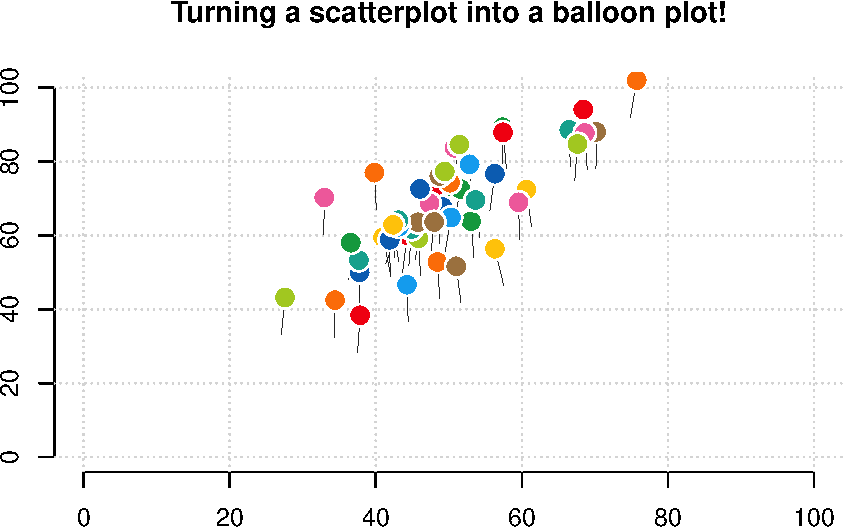
\includegraphics{YaRrr_files/figure-latex/balloonplot-1} 

}

\caption{A balloon plot}\label{fig:balloonplot}
\end{figure}

You can use colors and point sizes in a scatterplot to represent third
variables. In Figure \ref{fig:scatter3rd}, I'll plot the relationship
between pirate height and weight, but now I'll make the size and color
of each point reflect how many tattoos the pirate has

\begin{Shaded}
\begin{Highlighting}[]
\CommentTok{# Just the first 100 pirates}
\NormalTok{pirates.r <-}\StringTok{ }\NormalTok{pirates[}\DecValTok{1}\NormalTok{:}\DecValTok{100}\NormalTok{,]}

\KeywordTok{plot}\NormalTok{(}\DataTypeTok{x =} \NormalTok{pirates.r$height,}
     \DataTypeTok{y =} \NormalTok{pirates.r$weight,}
     \DataTypeTok{xlab =} \StringTok{"height"}\NormalTok{,}
     \DataTypeTok{ylab =} \StringTok{"weight"}\NormalTok{,}
     \DataTypeTok{main =} \StringTok{"Specifying point sizes and colors with a 3rd variable"}\NormalTok{,}
     \DataTypeTok{cex =} \NormalTok{pirates.r$tattoos  /}\StringTok{ }\DecValTok{8}\NormalTok{,          }\CommentTok{# Point size reflects how many tattoos they have}
     \DataTypeTok{col =} \KeywordTok{gray}\NormalTok{(}\DecValTok{1} \NormalTok{-}\StringTok{ }\NormalTok{pirates.r$tattoos /}\StringTok{ }\DecValTok{20}\NormalTok{)) }\CommentTok{# color reflects tattoos}

\KeywordTok{grid}\NormalTok{()}
\end{Highlighting}
\end{Shaded}

\begin{figure}

{\centering 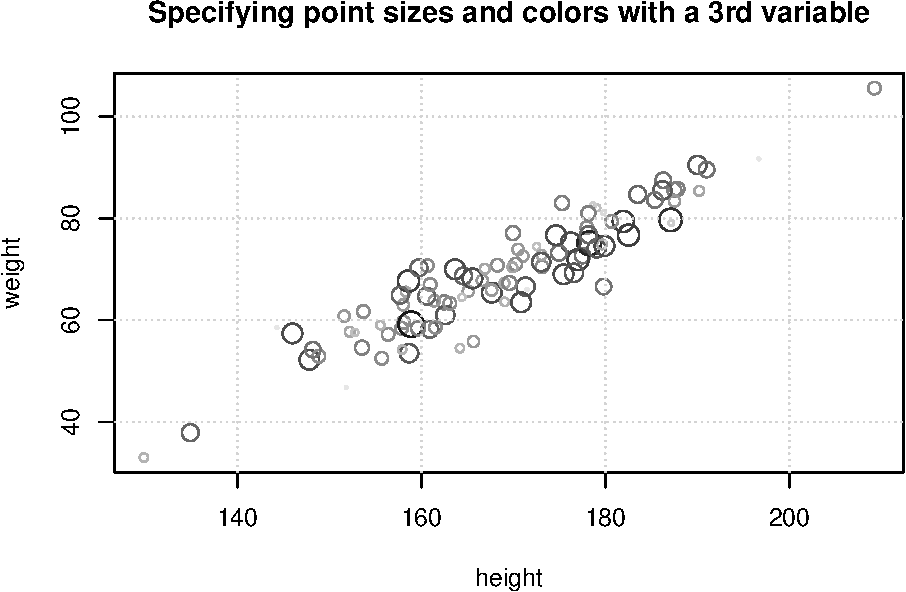
\includegraphics{YaRrr_files/figure-latex/scatter3rd-1} 

}

\caption{Specifying the size and color of points with a third variable.}\label{fig:scatter3rd}
\end{figure}

\section{Test your R might! Purdy
pictures}\label{test-your-r-might-purdy-pictures}

\begin{figure}

{\centering 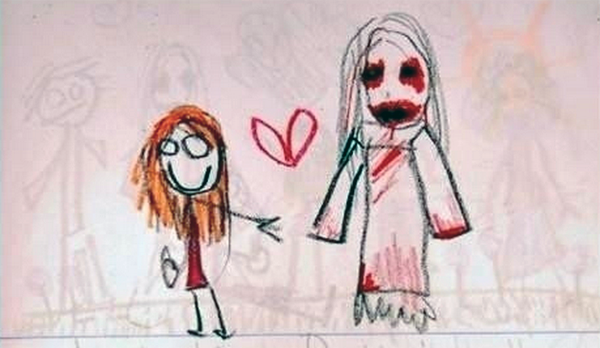
\includegraphics[width=0.75\linewidth]{images/scarydrawing} 

}

\end{figure}

\begin{enumerate}
\def\labelenumi{\arabic{enumi}.}
\tightlist
\item
  The \texttt{BeardLengths} dataframe (contained in the \texttt{yarrr}
  package or online at
  \url{https://github.com/ndphillips/ThePiratesGuideToR/raw/master/data/BeardLengths.txt})
  contains data on the lengths of beards from 3 different pirate ships.
  Calculate the average beard length for each ship using
  \texttt{aggregate()}, then create the following barplot:
\end{enumerate}

\begin{center}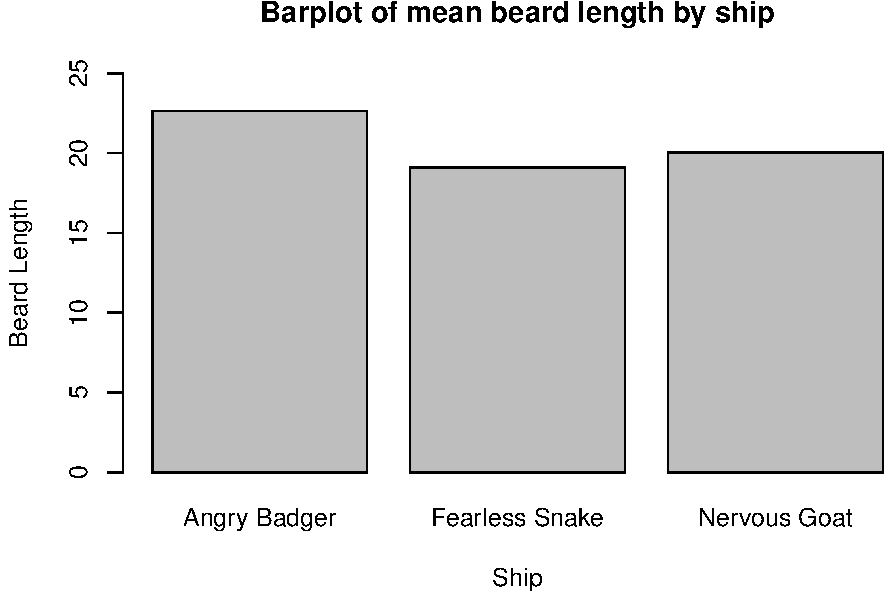
\includegraphics{YaRrr_files/figure-latex/unnamed-chunk-33-1} \end{center}

\begin{enumerate}
\def\labelenumi{\arabic{enumi}.}
\setcounter{enumi}{1}
\tightlist
\item
  Now using the entire \texttt{BeardLengths} dataframe, create the
  following pirateplot:
\end{enumerate}

\begin{center}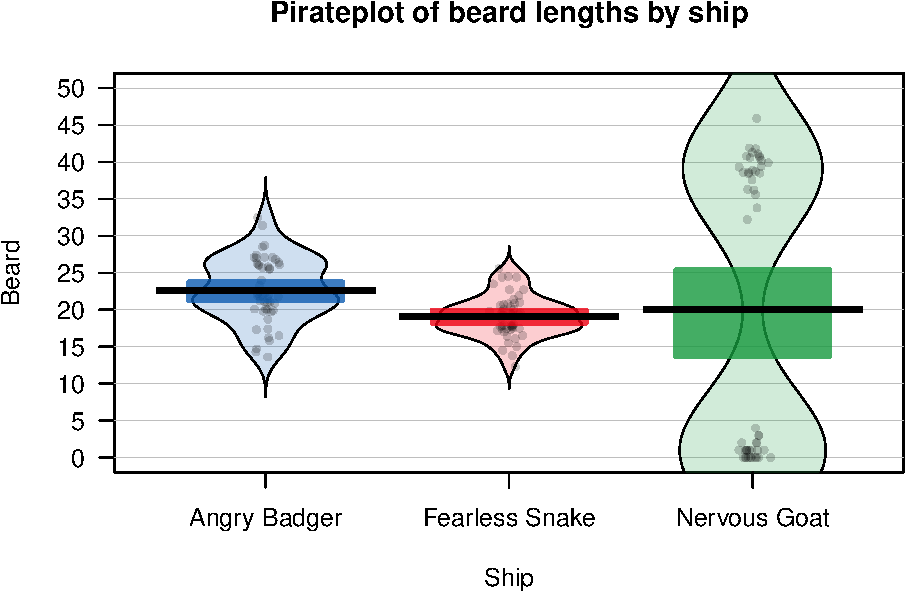
\includegraphics{YaRrr_files/figure-latex/unnamed-chunk-34-1} \end{center}

\begin{enumerate}
\def\labelenumi{\arabic{enumi}.}
\setcounter{enumi}{2}
\tightlist
\item
  Using the \texttt{pirates} dataset, create the following scatterplot
  showing the relationship between a pirate's age and how many parrot's
  (s)he has owned (hint: to make the points solid and transparent, use
  \texttt{pch\ =\ 16}, and
  \texttt{col\ =\ gray(level\ =\ .5,\ alpha\ =\ .1)}).
\end{enumerate}

\begin{center}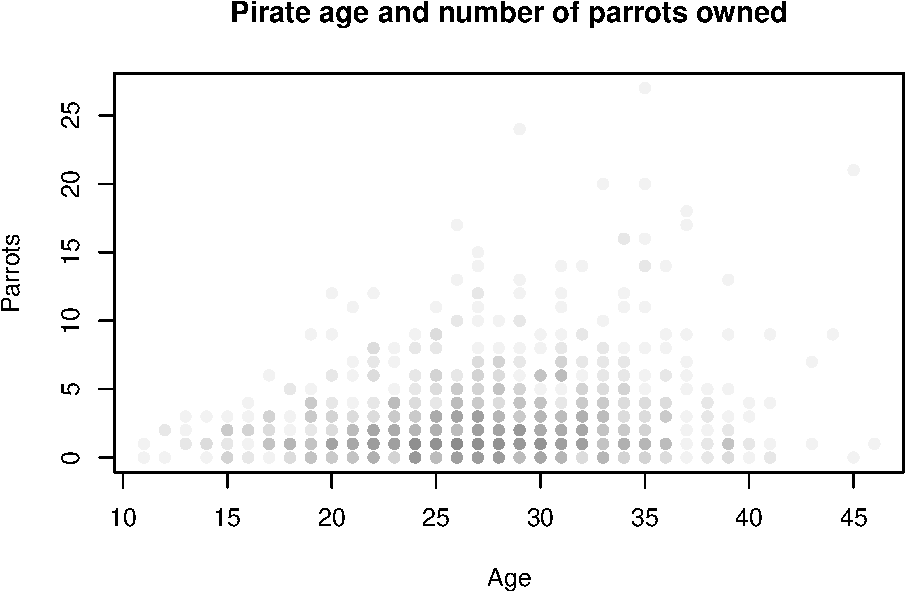
\includegraphics{YaRrr_files/figure-latex/unnamed-chunk-35-1} \end{center}

\chapter{Plotting (II)}\label{plotting2}

\chapter{Hypothesis Tests}\label{htests}

\chapter{ANOVA}\label{anova}

\chapter{Regression}\label{regression}

\chapter{Custom functions}\label{functions}

\chapter{Loops}\label{loops}

\chapter{Solutions}\label{solutions}

\chapter{Placeholder}\label{placeholder}

\bibliography{packages.bib,book.bib}


\end{document}
